\chapter{Reweight Dedicated TT MC Samples for the Estimation of theoretical uncertainties}

\begin{figure}
    \centering
    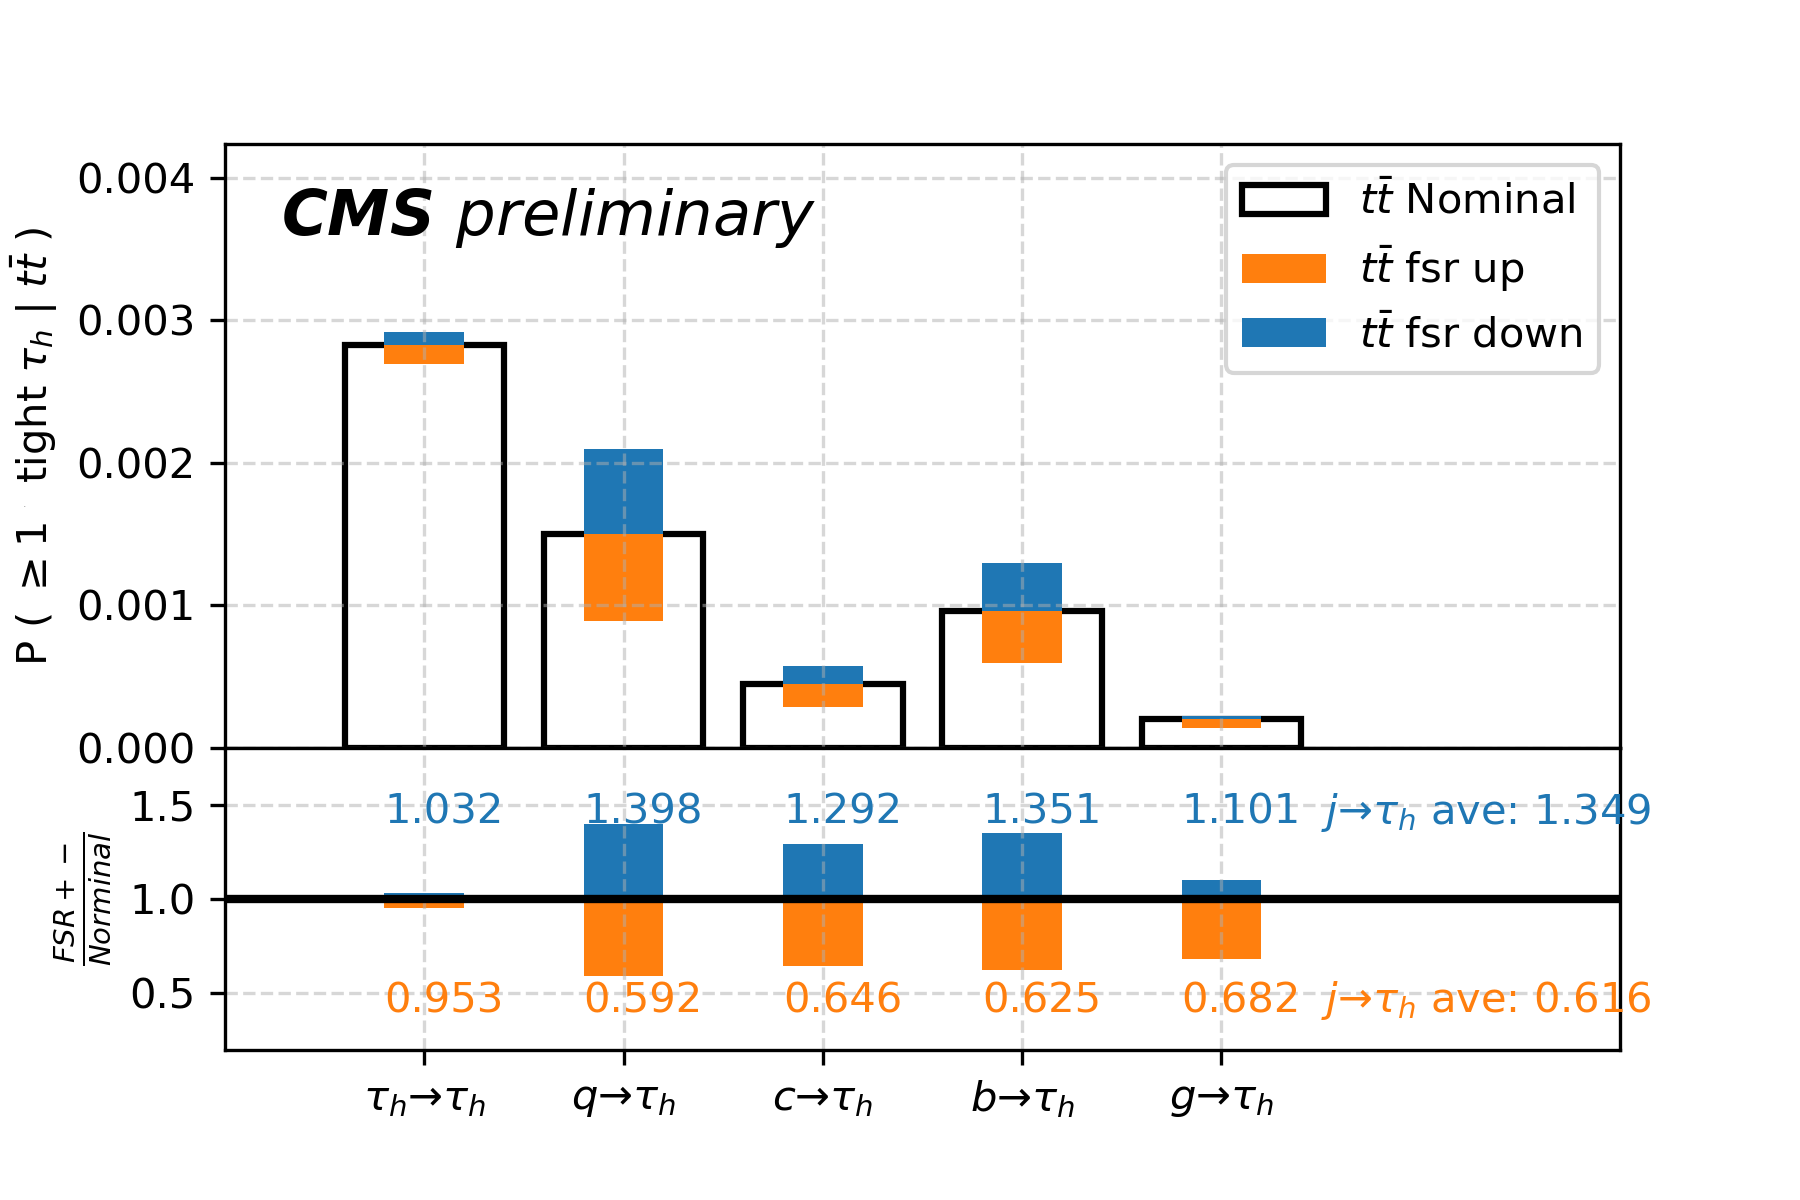
\includegraphics[width=0.49\textwidth]{chapters/Appendix/sectionTTSyst/figures/2020_MCRatio_fsr_tauGenFlavor_tauTight.png}
    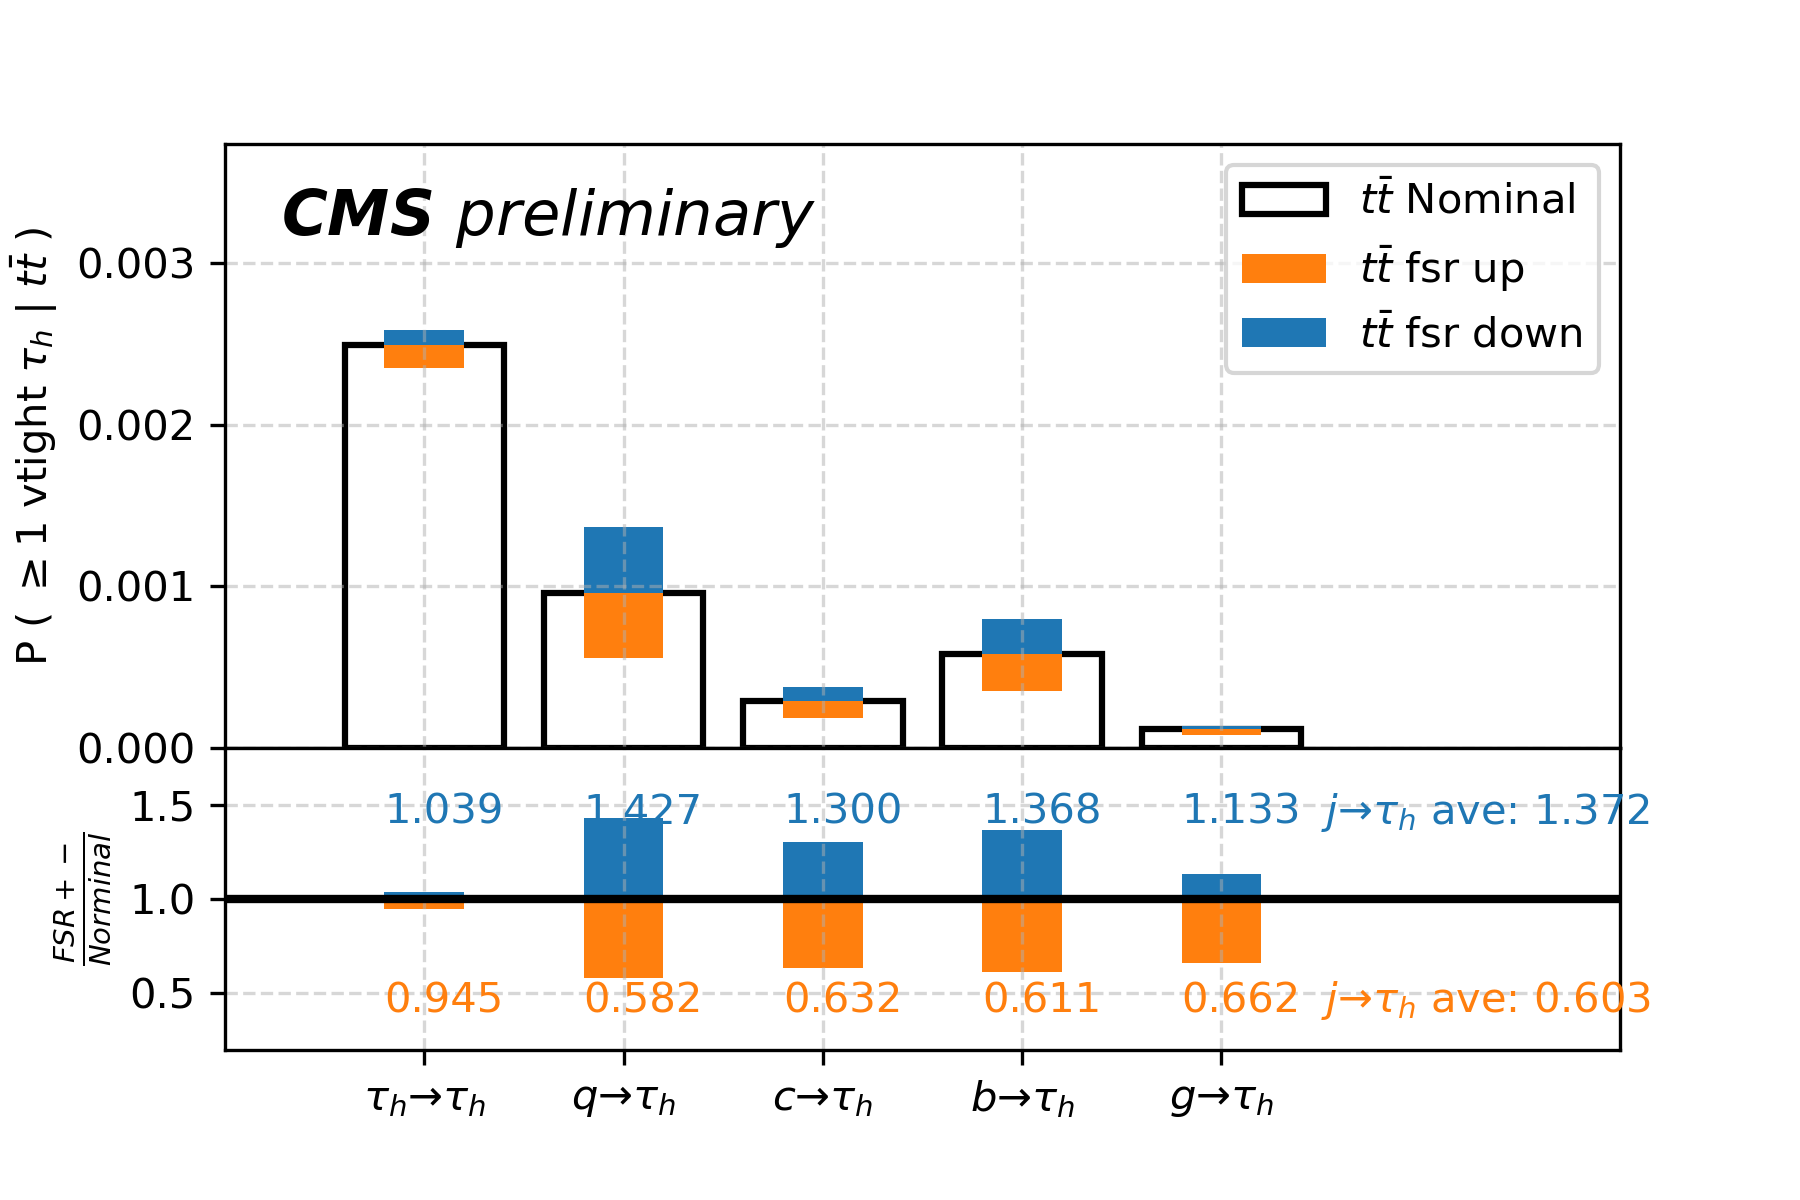
\includegraphics[width=0.49\textwidth]{chapters/Appendix/sectionTTSyst/figures/2020_MCRatio_fsr_tauGenFlavor_tauVTight.png}
    \caption{Reweight $\tau_h$ and $j \to \tau_h$ efficiencies in the dedicated FSR ttbar samples}
    \label{fig:appendix:reweighttt:sf}
\end{figure}

\begin{figure}
    \centering
    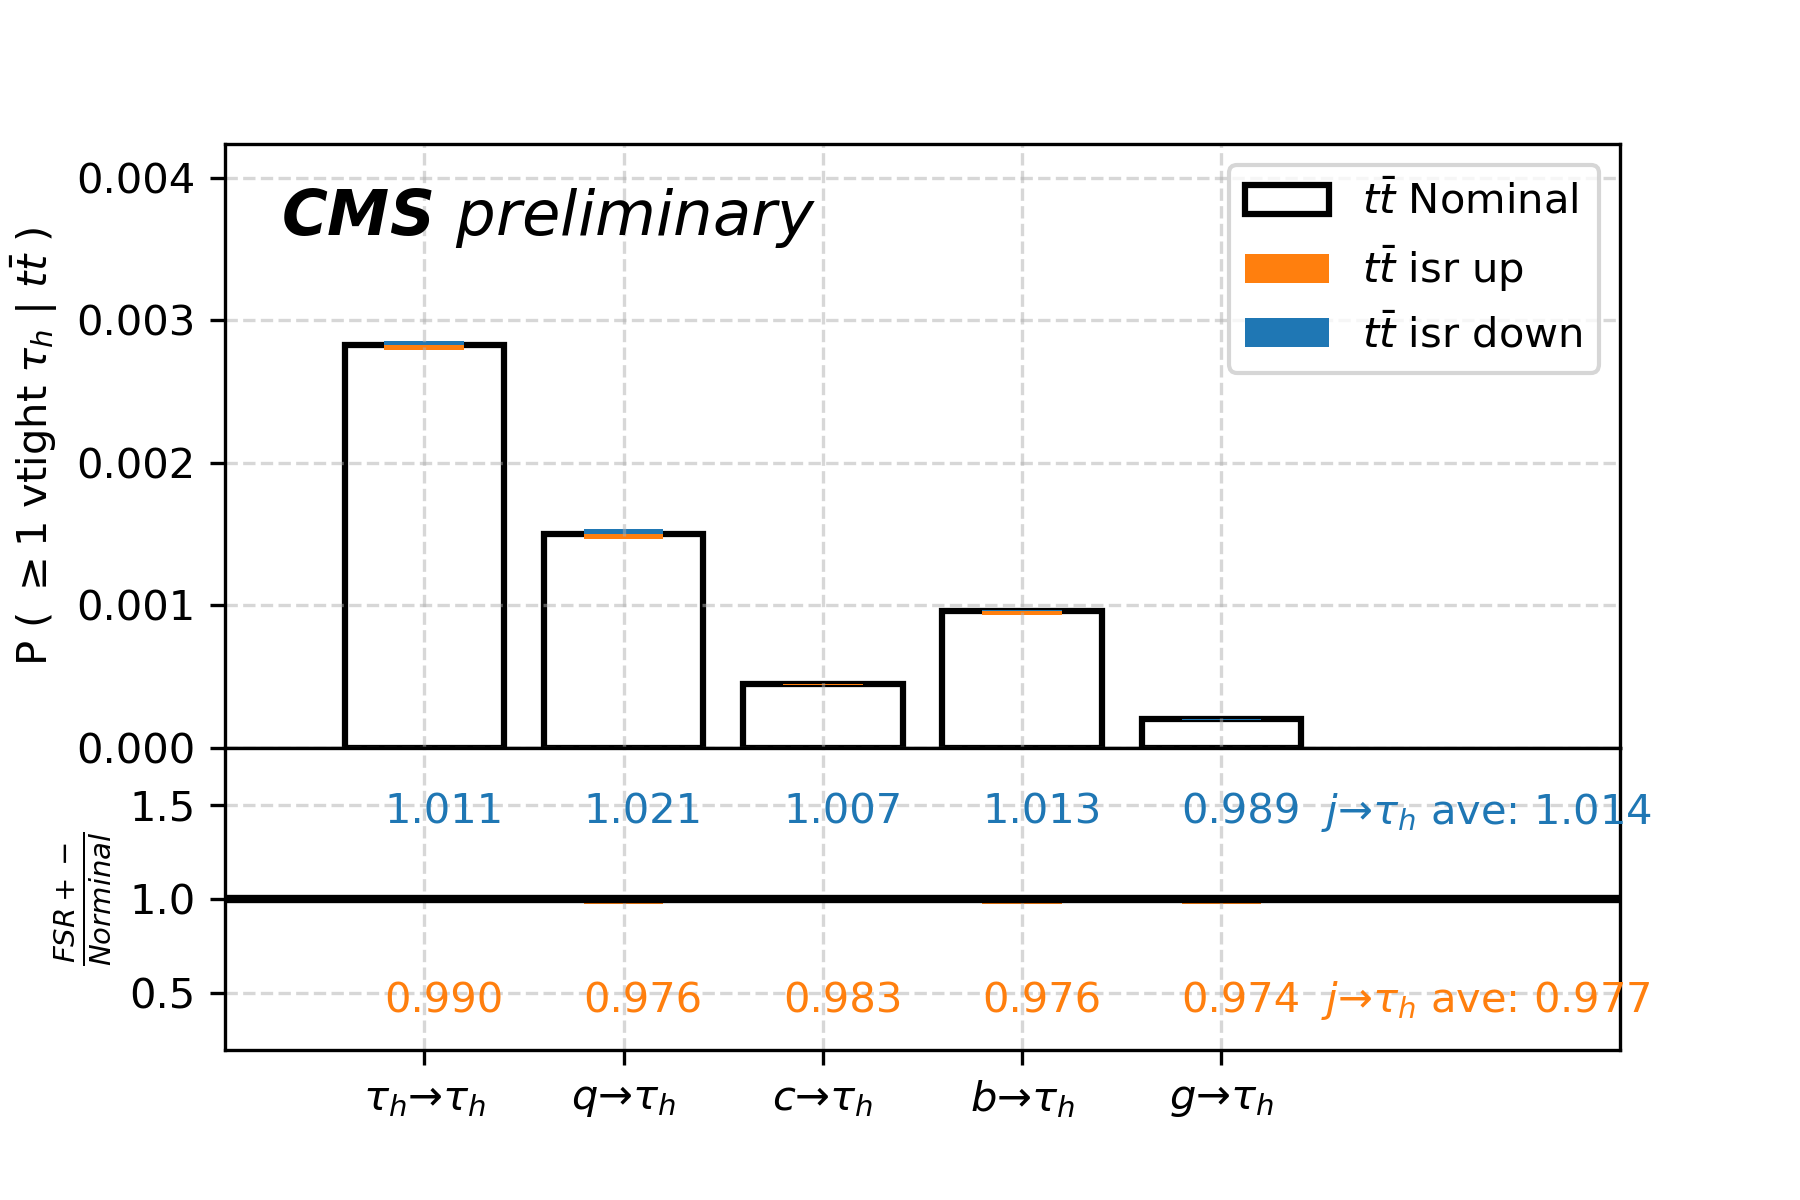
\includegraphics[width=0.49\textwidth]{chapters/Appendix/sectionTTSyst/figures/2020_MCRatio_isr_tauGenFlavor_tauTight.png}
    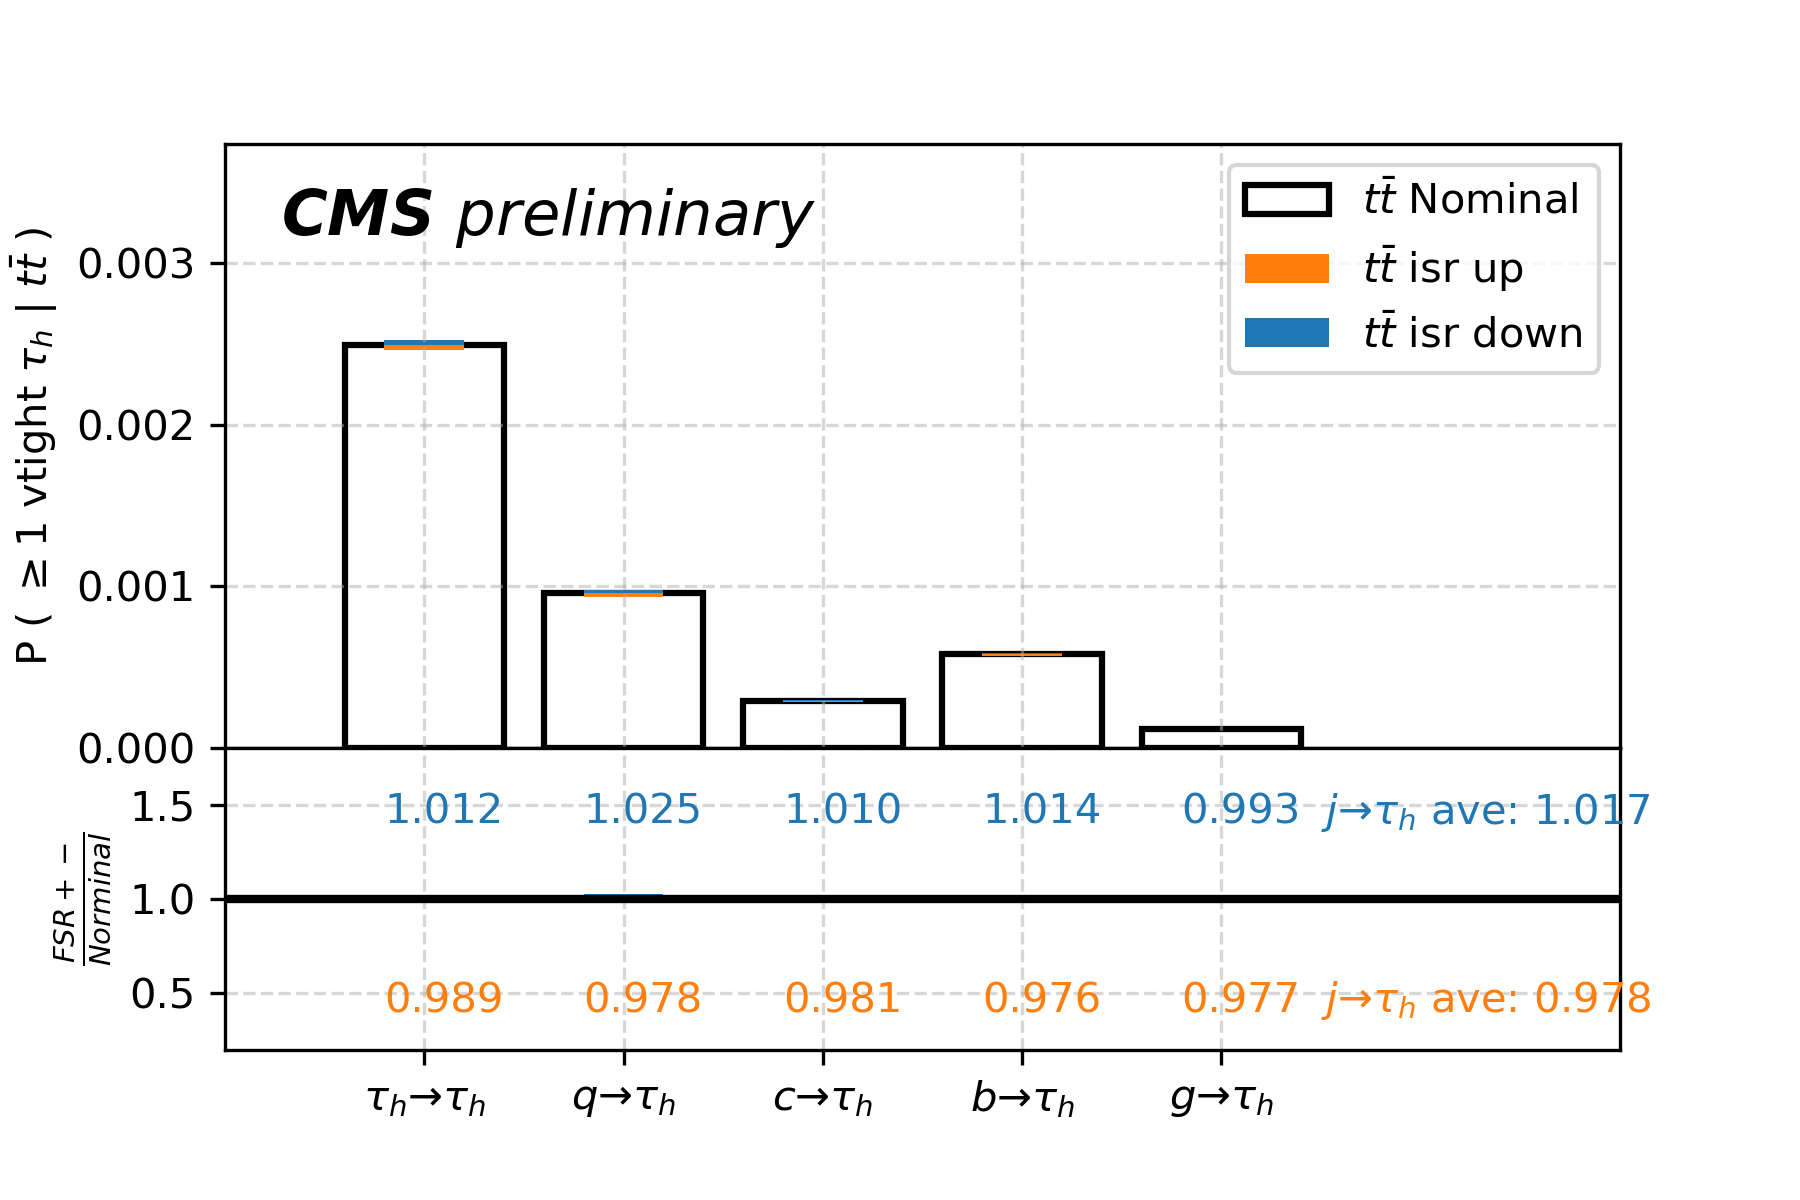
\includegraphics[width=0.49\textwidth]{chapters/Appendix/sectionTTSyst/figures/2020_MCRatio_isr_tauGenFlavor_tauVTight.png}
    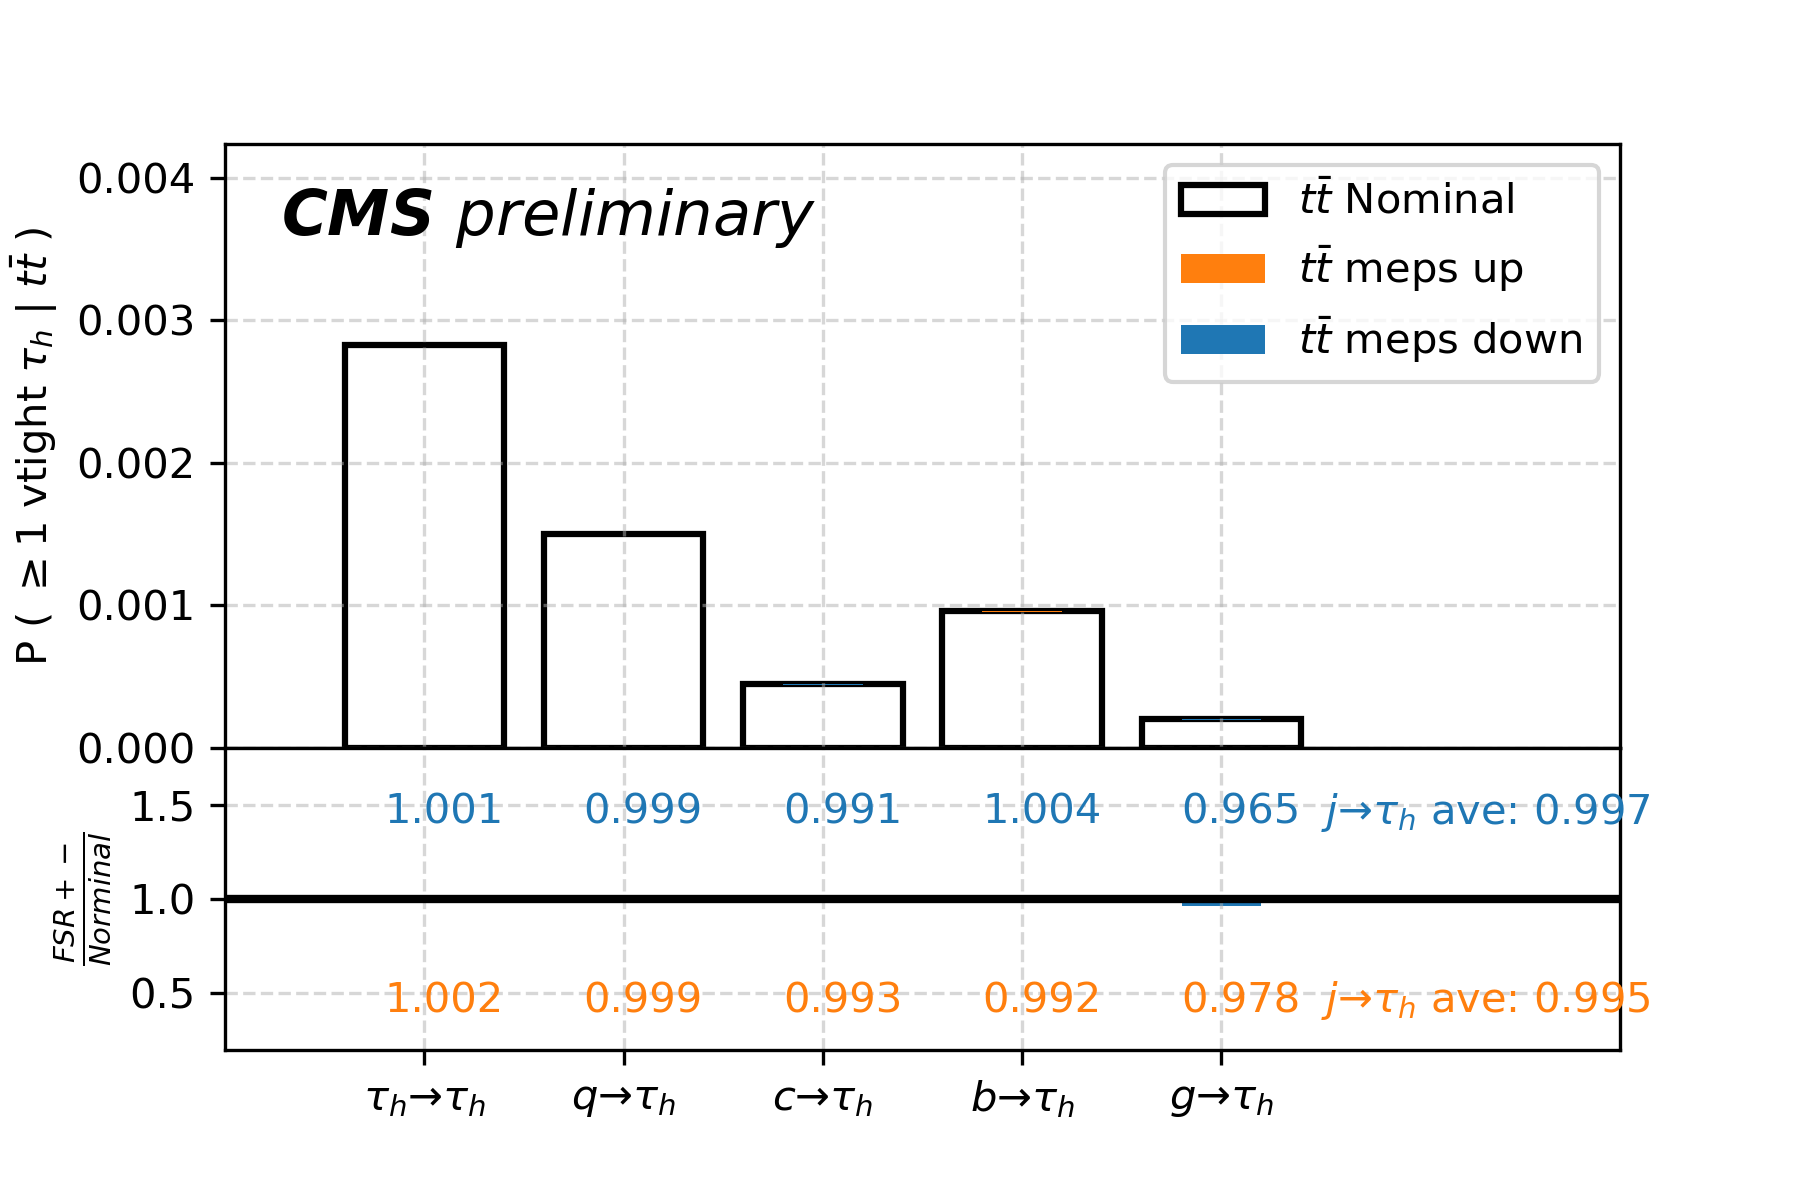
\includegraphics[width=0.49\textwidth]{chapters/Appendix/sectionTTSyst/figures/2020_MCRatio_meps_tauGenFlavor_tauTight.png}
    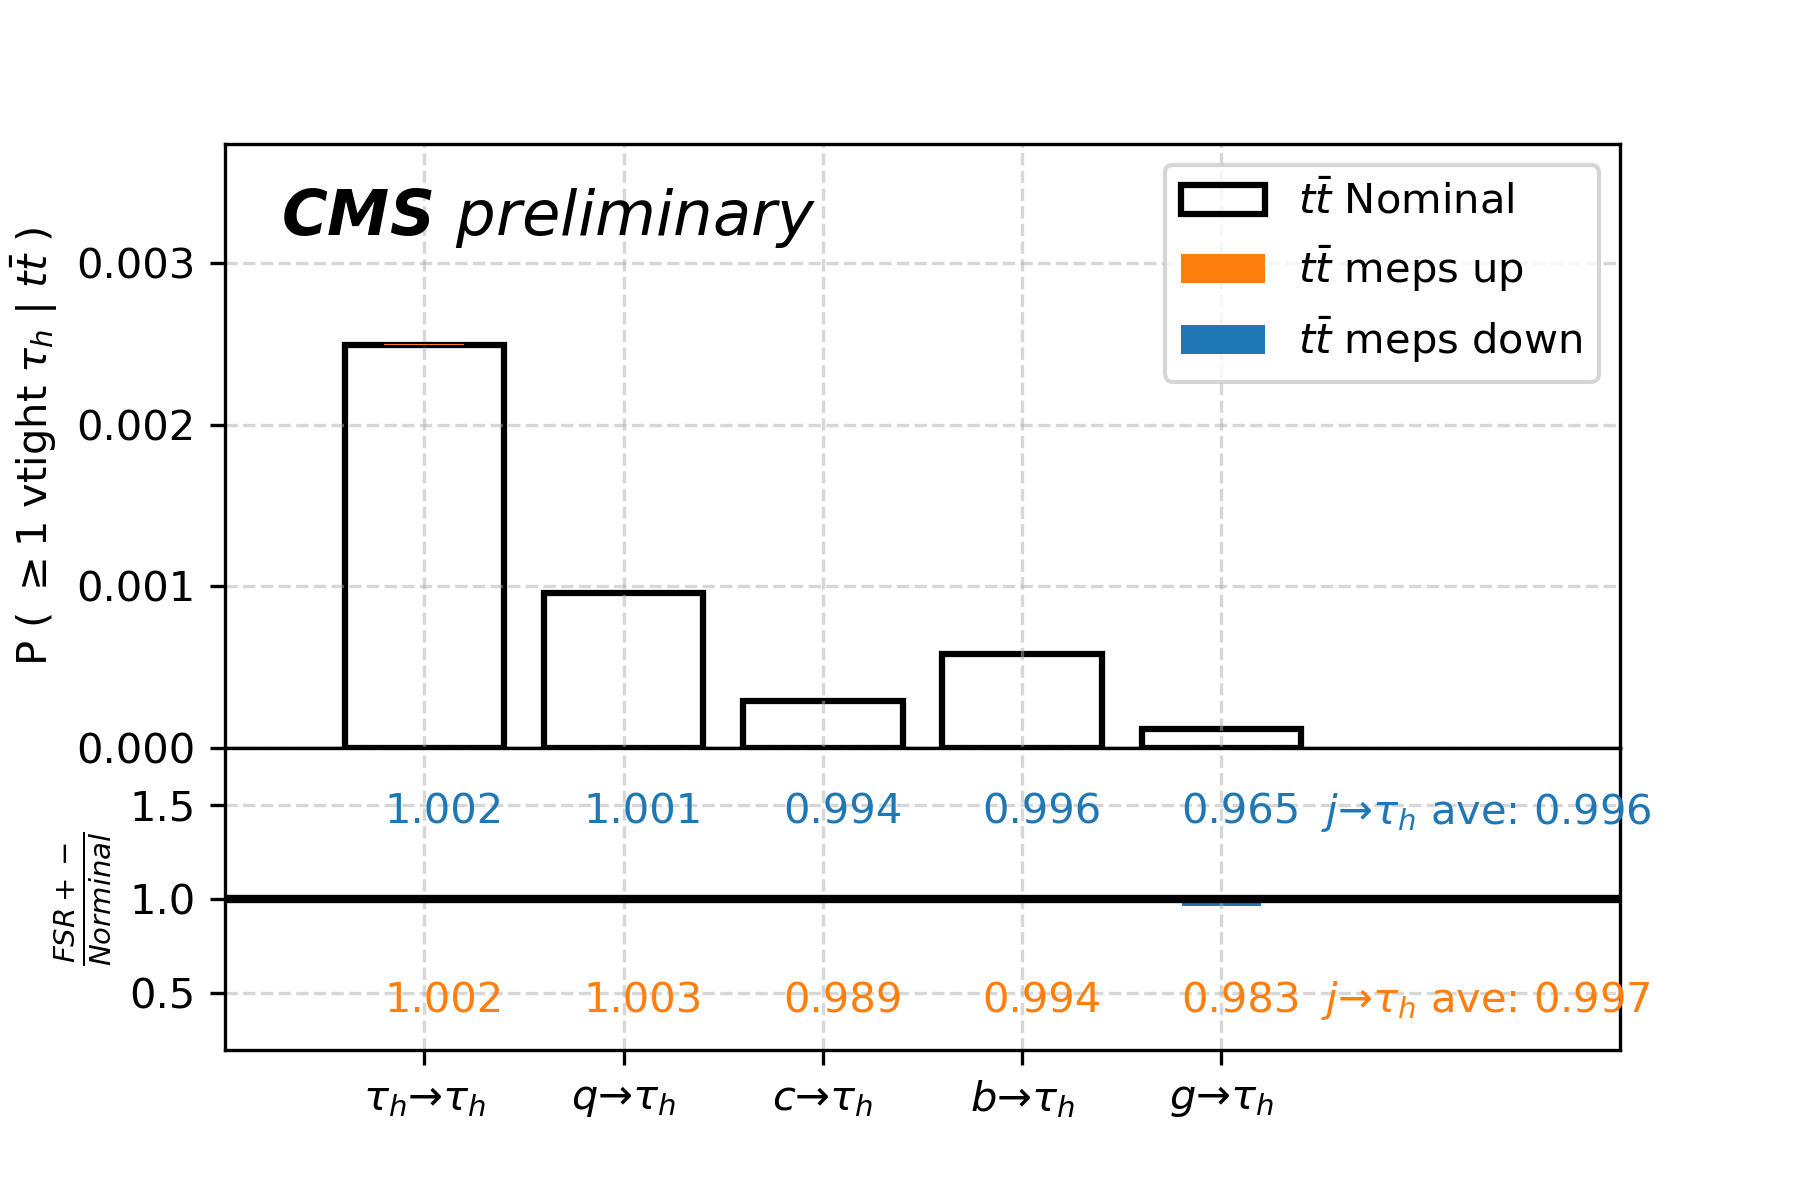
\includegraphics[width=0.49\textwidth]{chapters/Appendix/sectionTTSyst/figures/2020_MCRatio_meps_tauGenFlavor_tauVTight.png}
    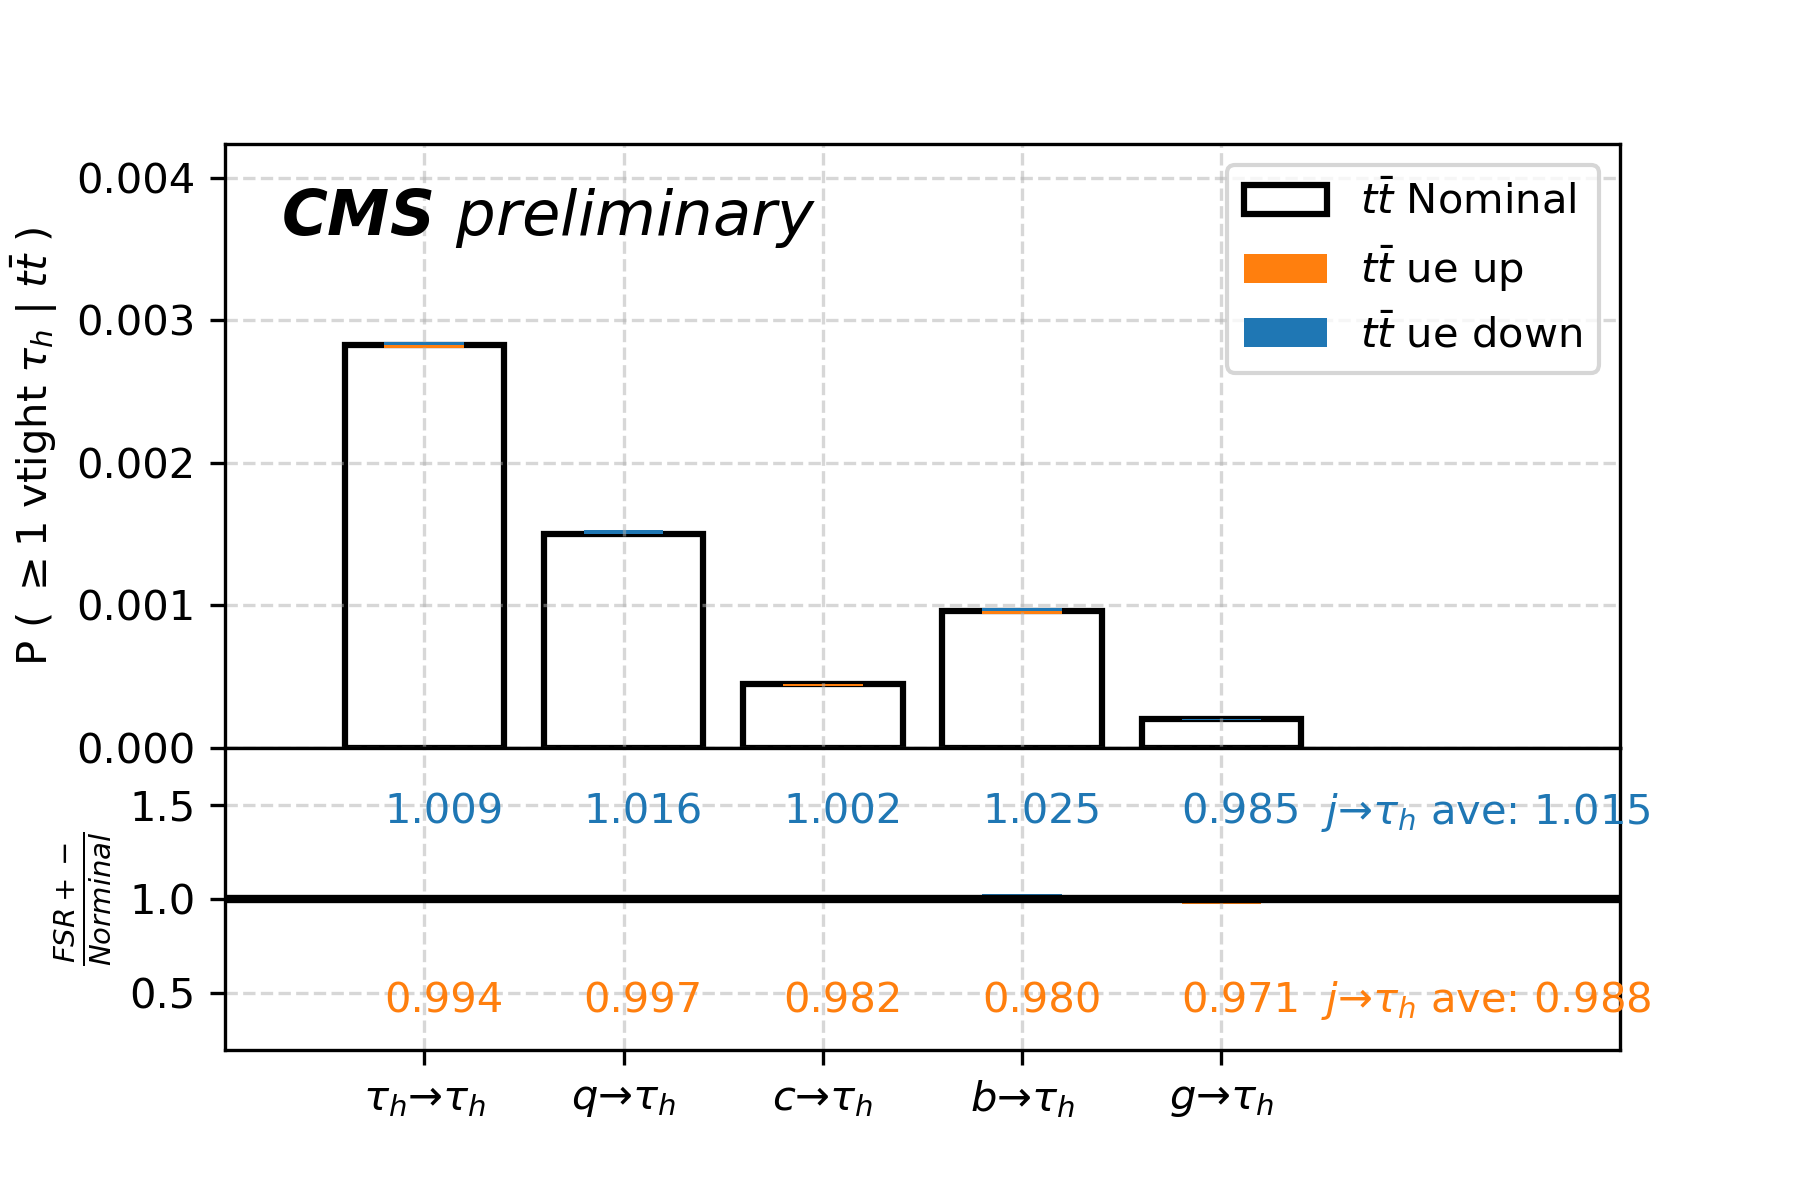
\includegraphics[width=0.49\textwidth]{chapters/Appendix/sectionTTSyst/figures/2020_MCRatio_ue_tauGenFlavor_tauTight.png}
    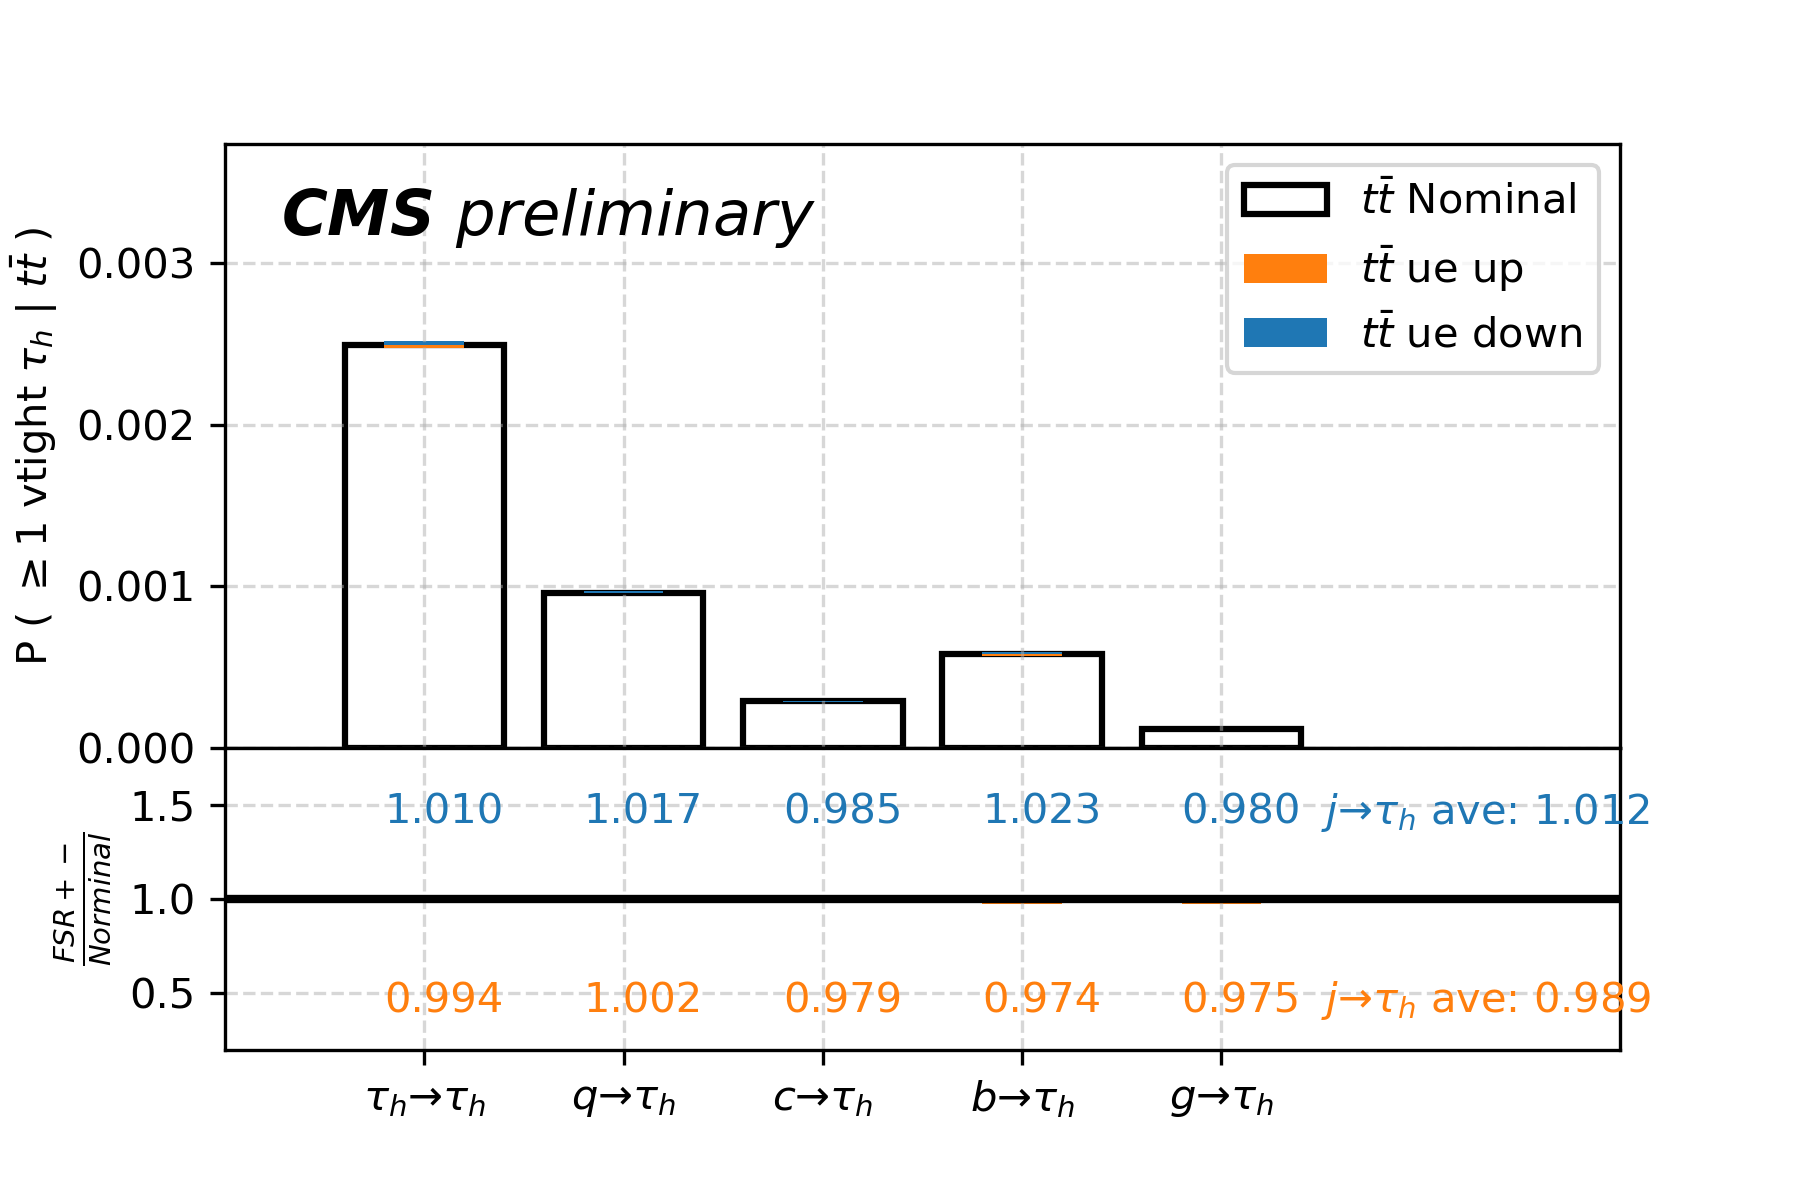
\includegraphics[width=0.49\textwidth]{chapters/Appendix/sectionTTSyst/figures/2020_MCRatio_ue_tauGenFlavor_tauVTight.png}
    \caption{Reweight $\tau_h$ and $j \to \tau_h$ efficiencies in the dedicated ISF, MEPS, UE ttbar samples}
    \label{fig:appendix:reweighttt:sf}
\end{figure}


\begin{figure}
    \centering
    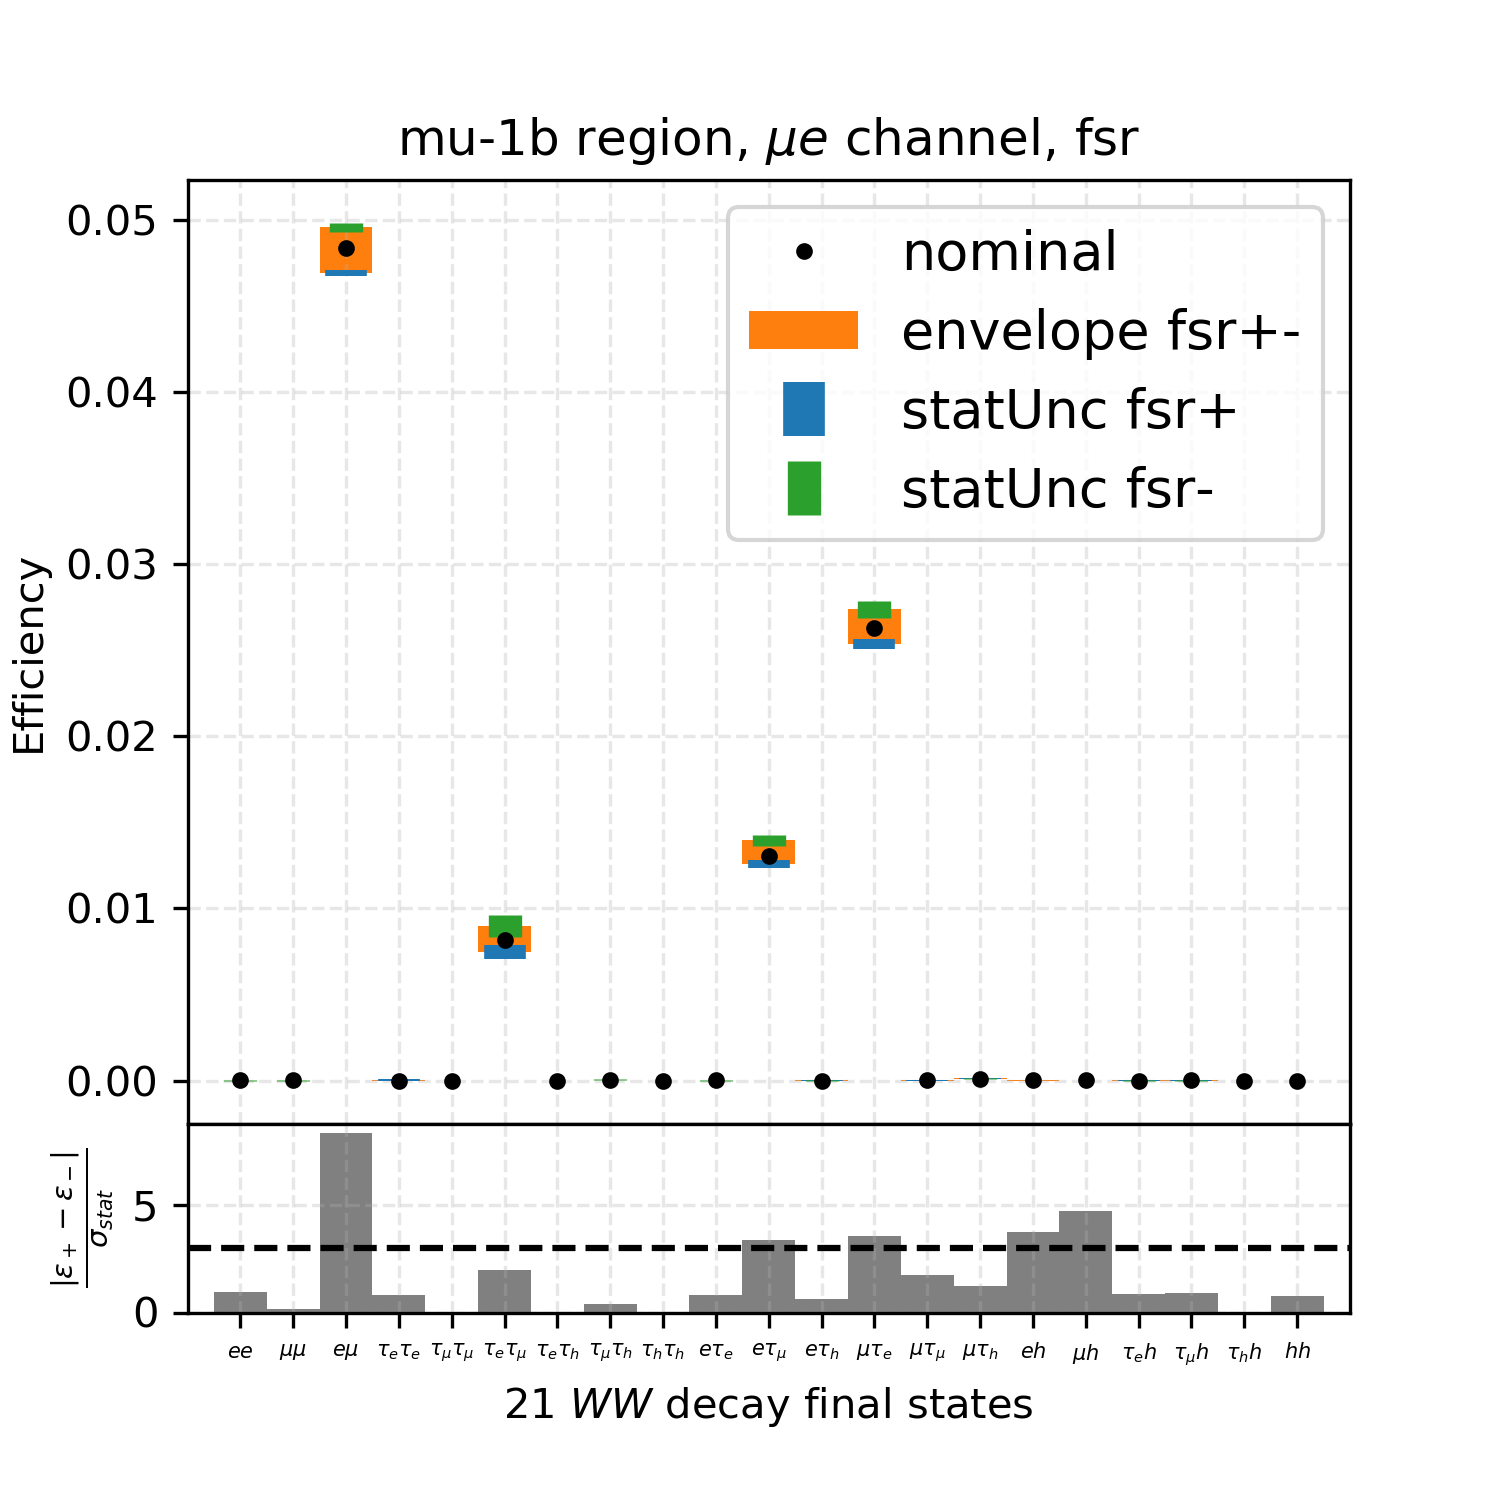
\includegraphics[width=0.24\textwidth]{chapters/Appendix/sectionTTSyst/figures/afterCorr/icata0_ch0_fsr.png}
    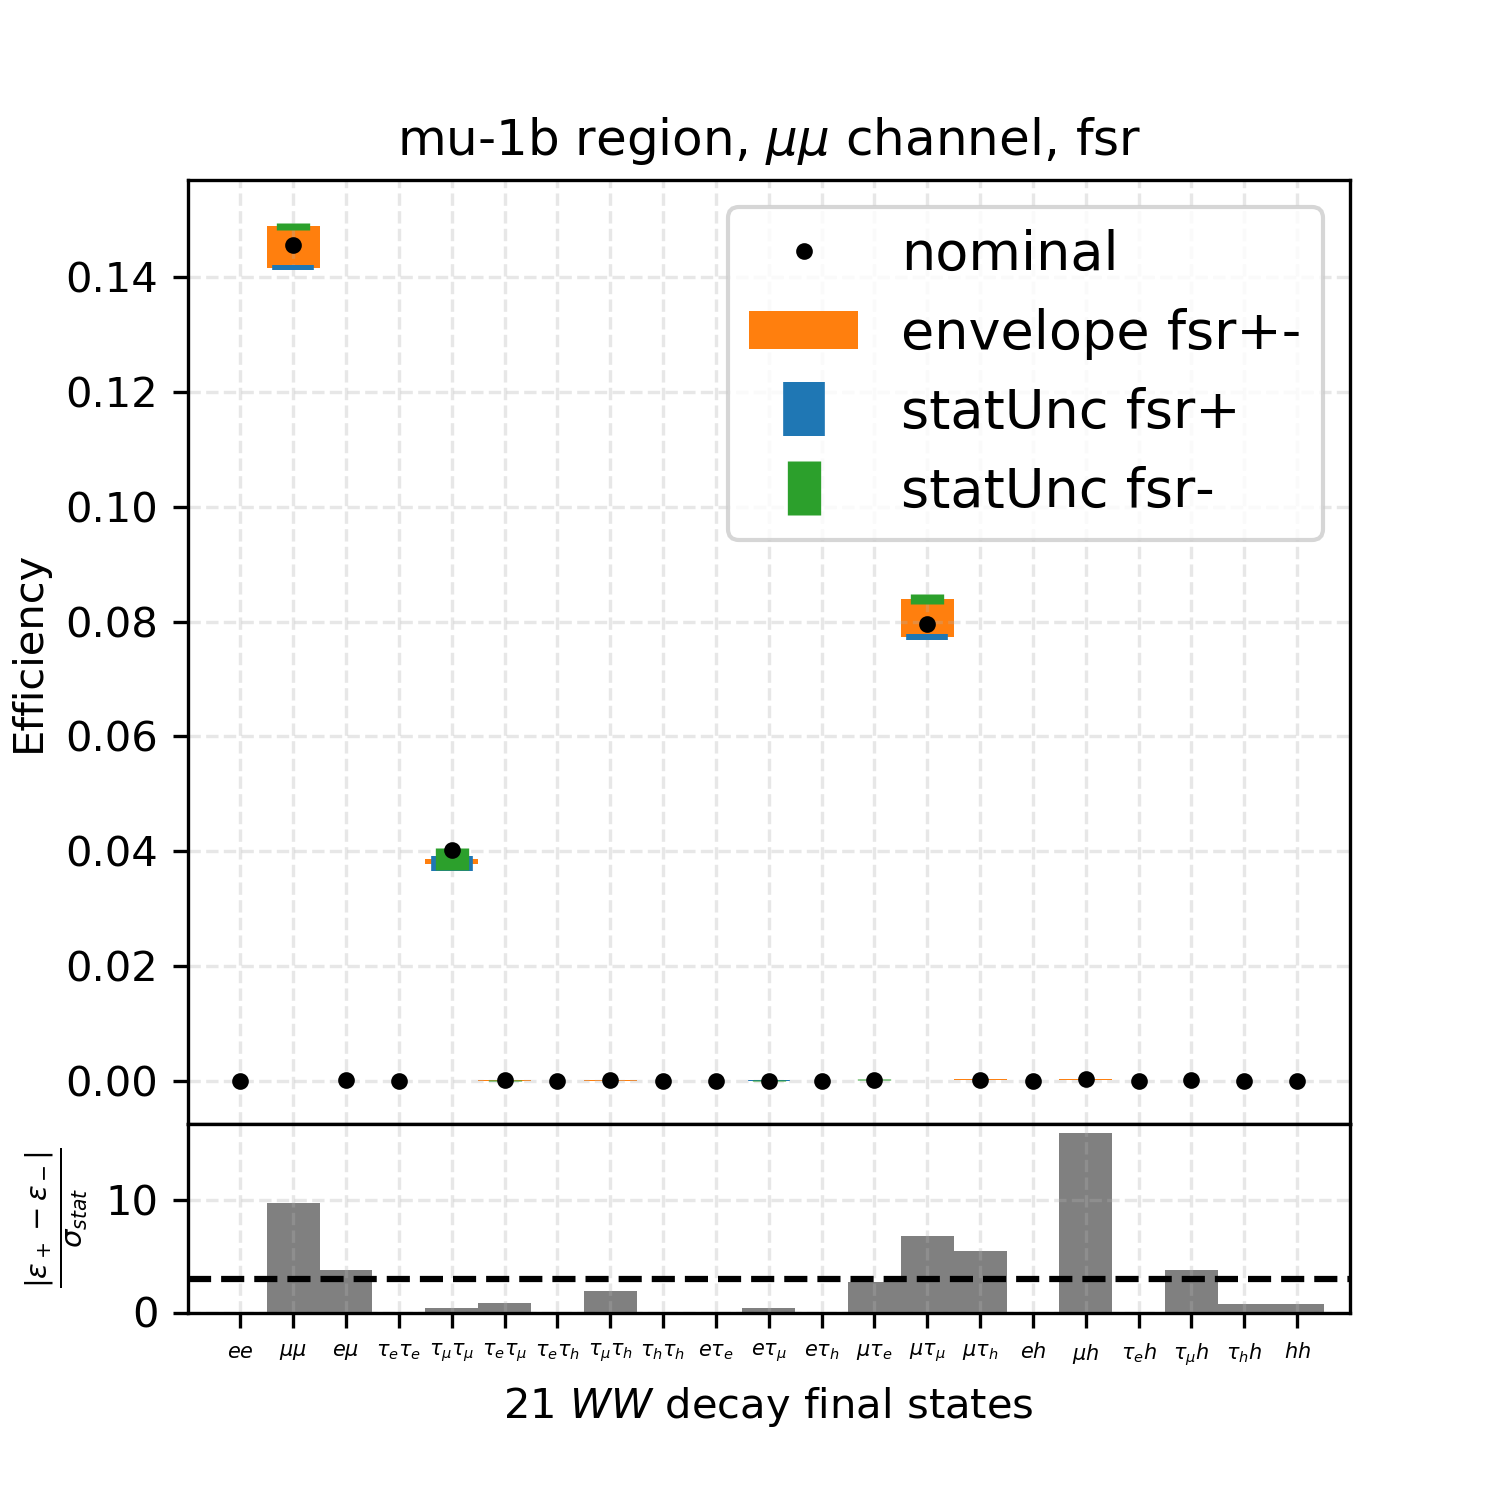
\includegraphics[width=0.24\textwidth]{chapters/Appendix/sectionTTSyst/figures/afterCorr/icata0_ch1_fsr.png}
    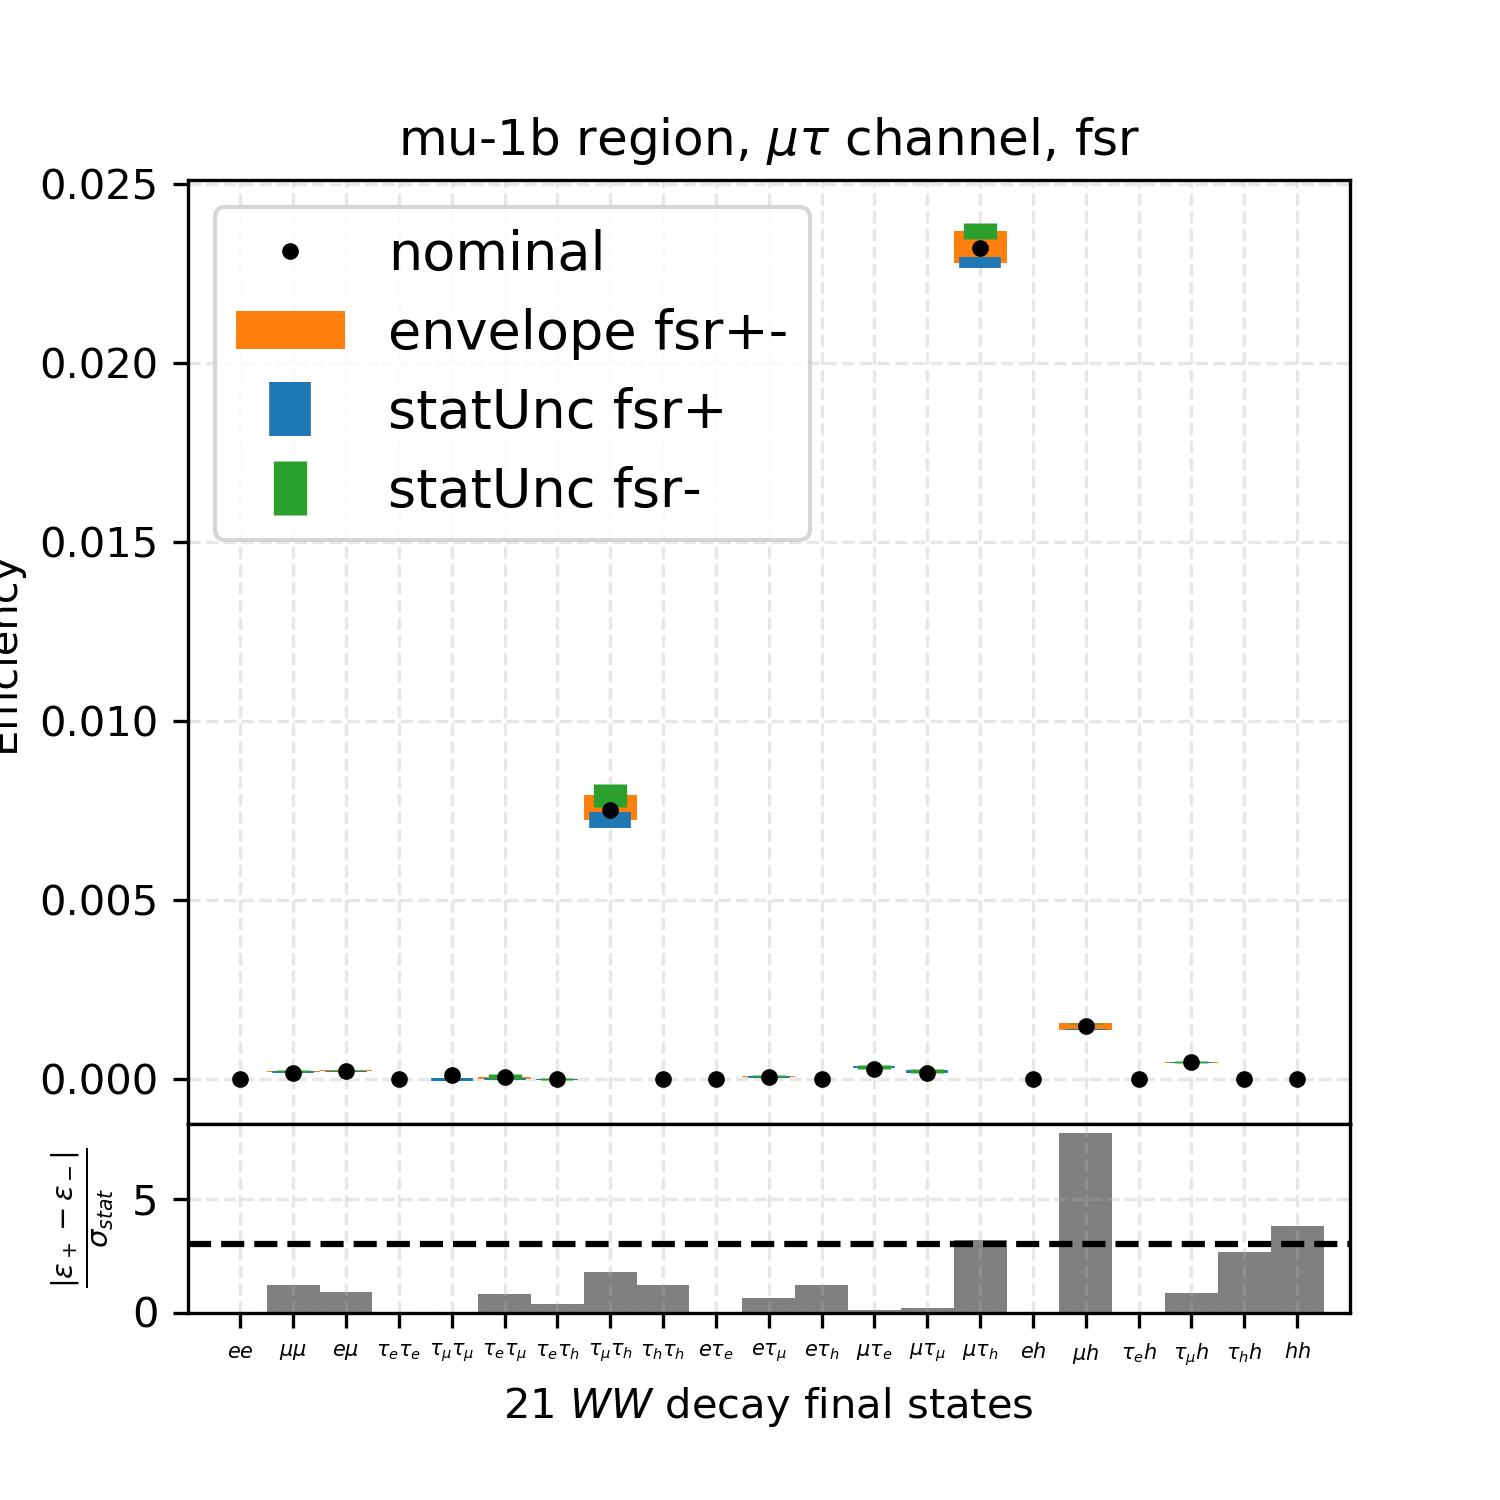
\includegraphics[width=0.24\textwidth]{chapters/Appendix/sectionTTSyst/figures/afterCorr/icata0_ch2_fsr.png}
    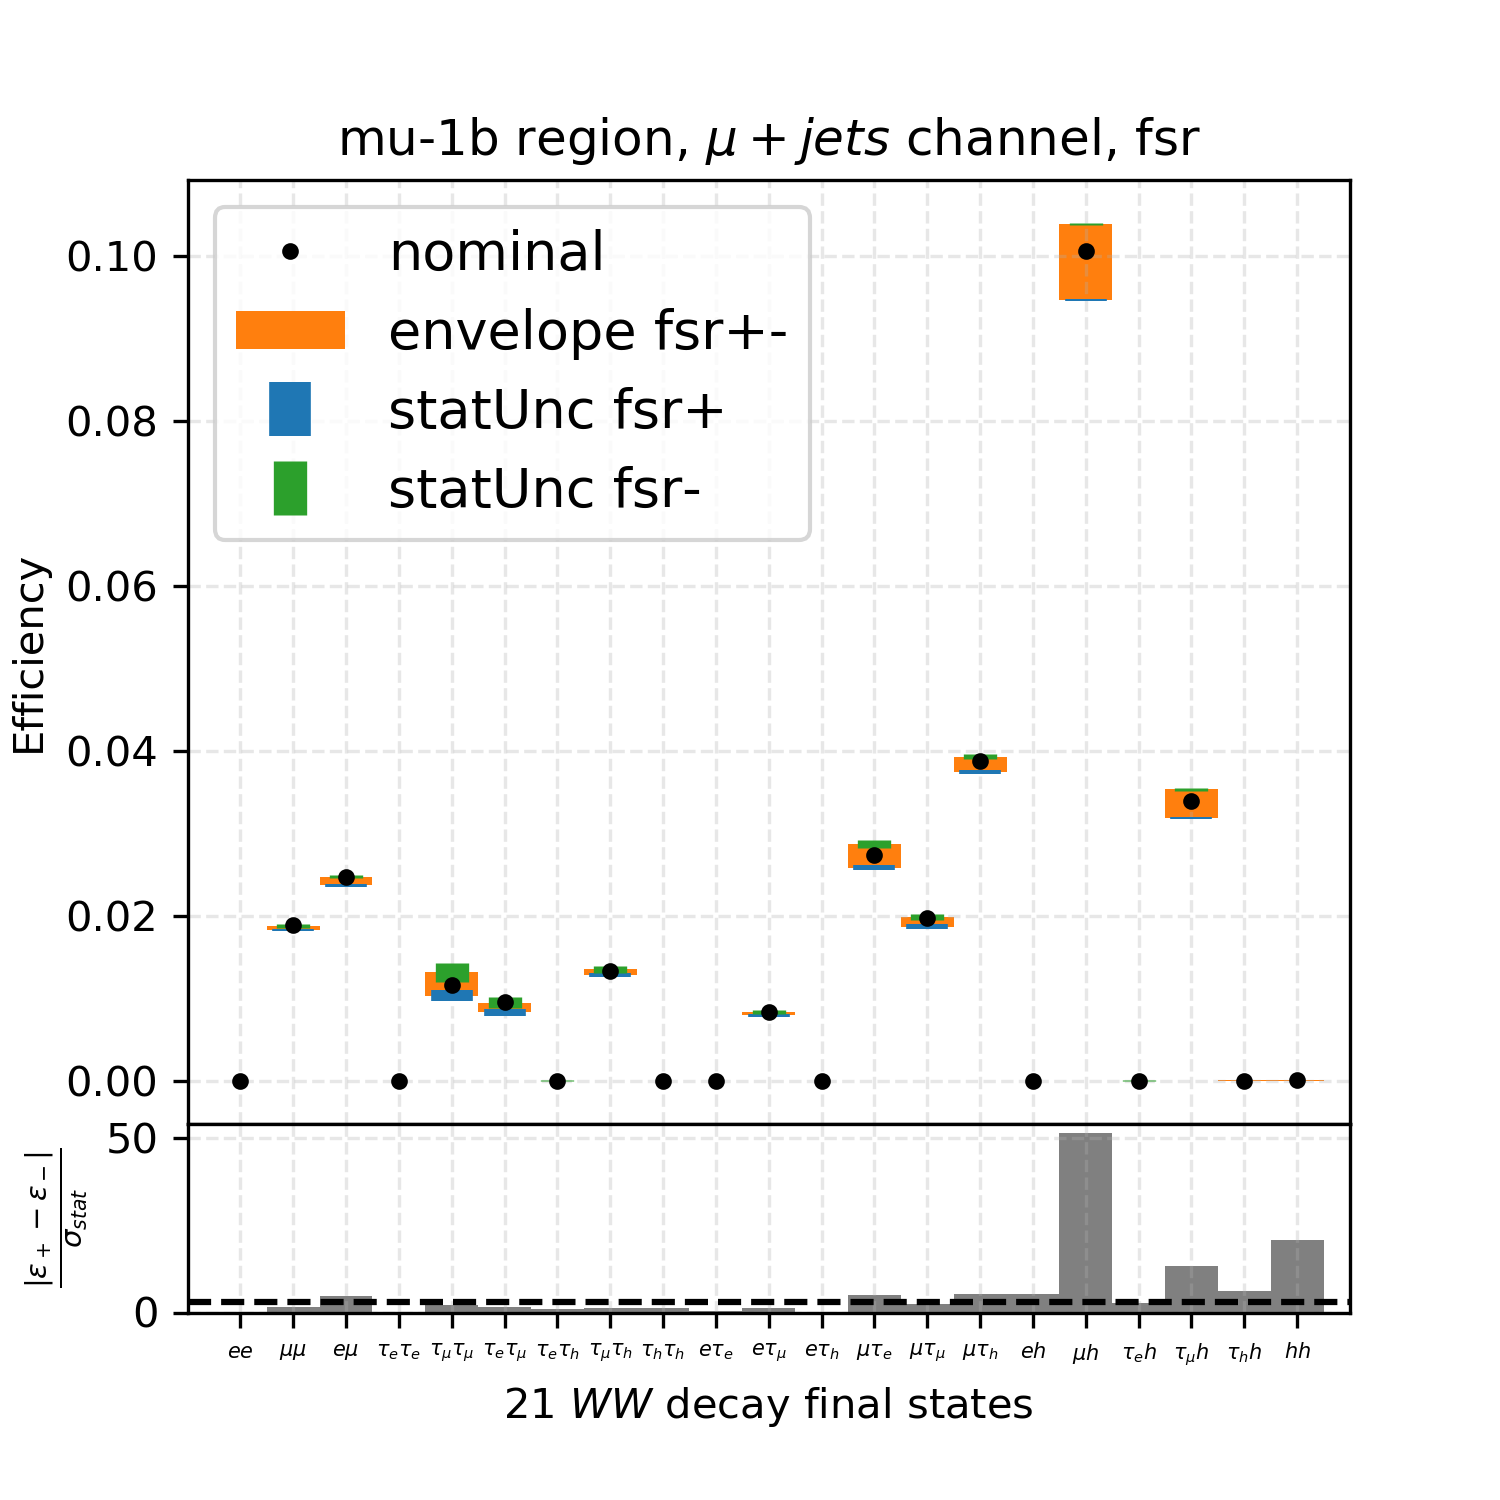
\includegraphics[width=0.24\textwidth]{chapters/Appendix/sectionTTSyst/figures/afterCorr/icata0_ch3_fsr.png}

    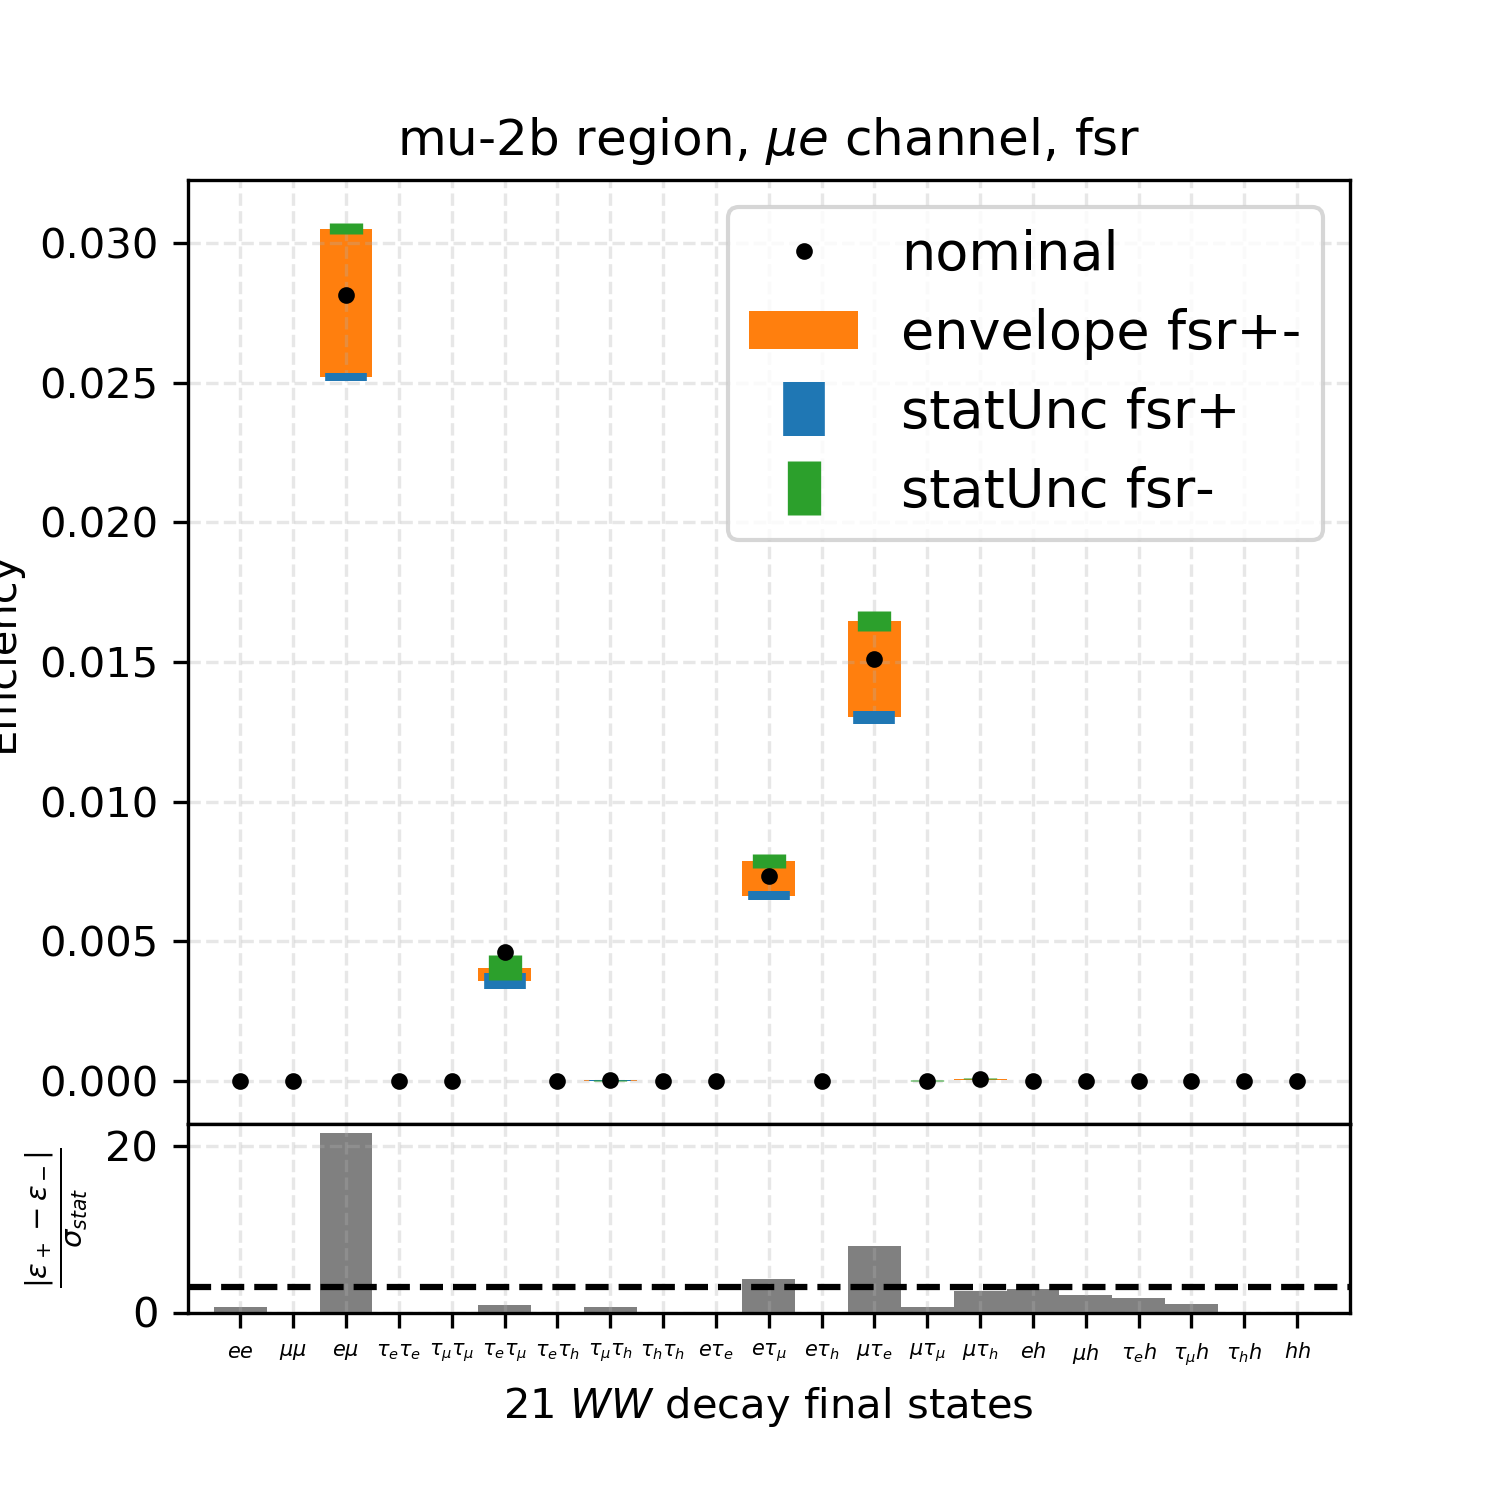
\includegraphics[width=0.24\textwidth]{chapters/Appendix/sectionTTSyst/figures/afterCorr/icata1_ch0_fsr.png}
    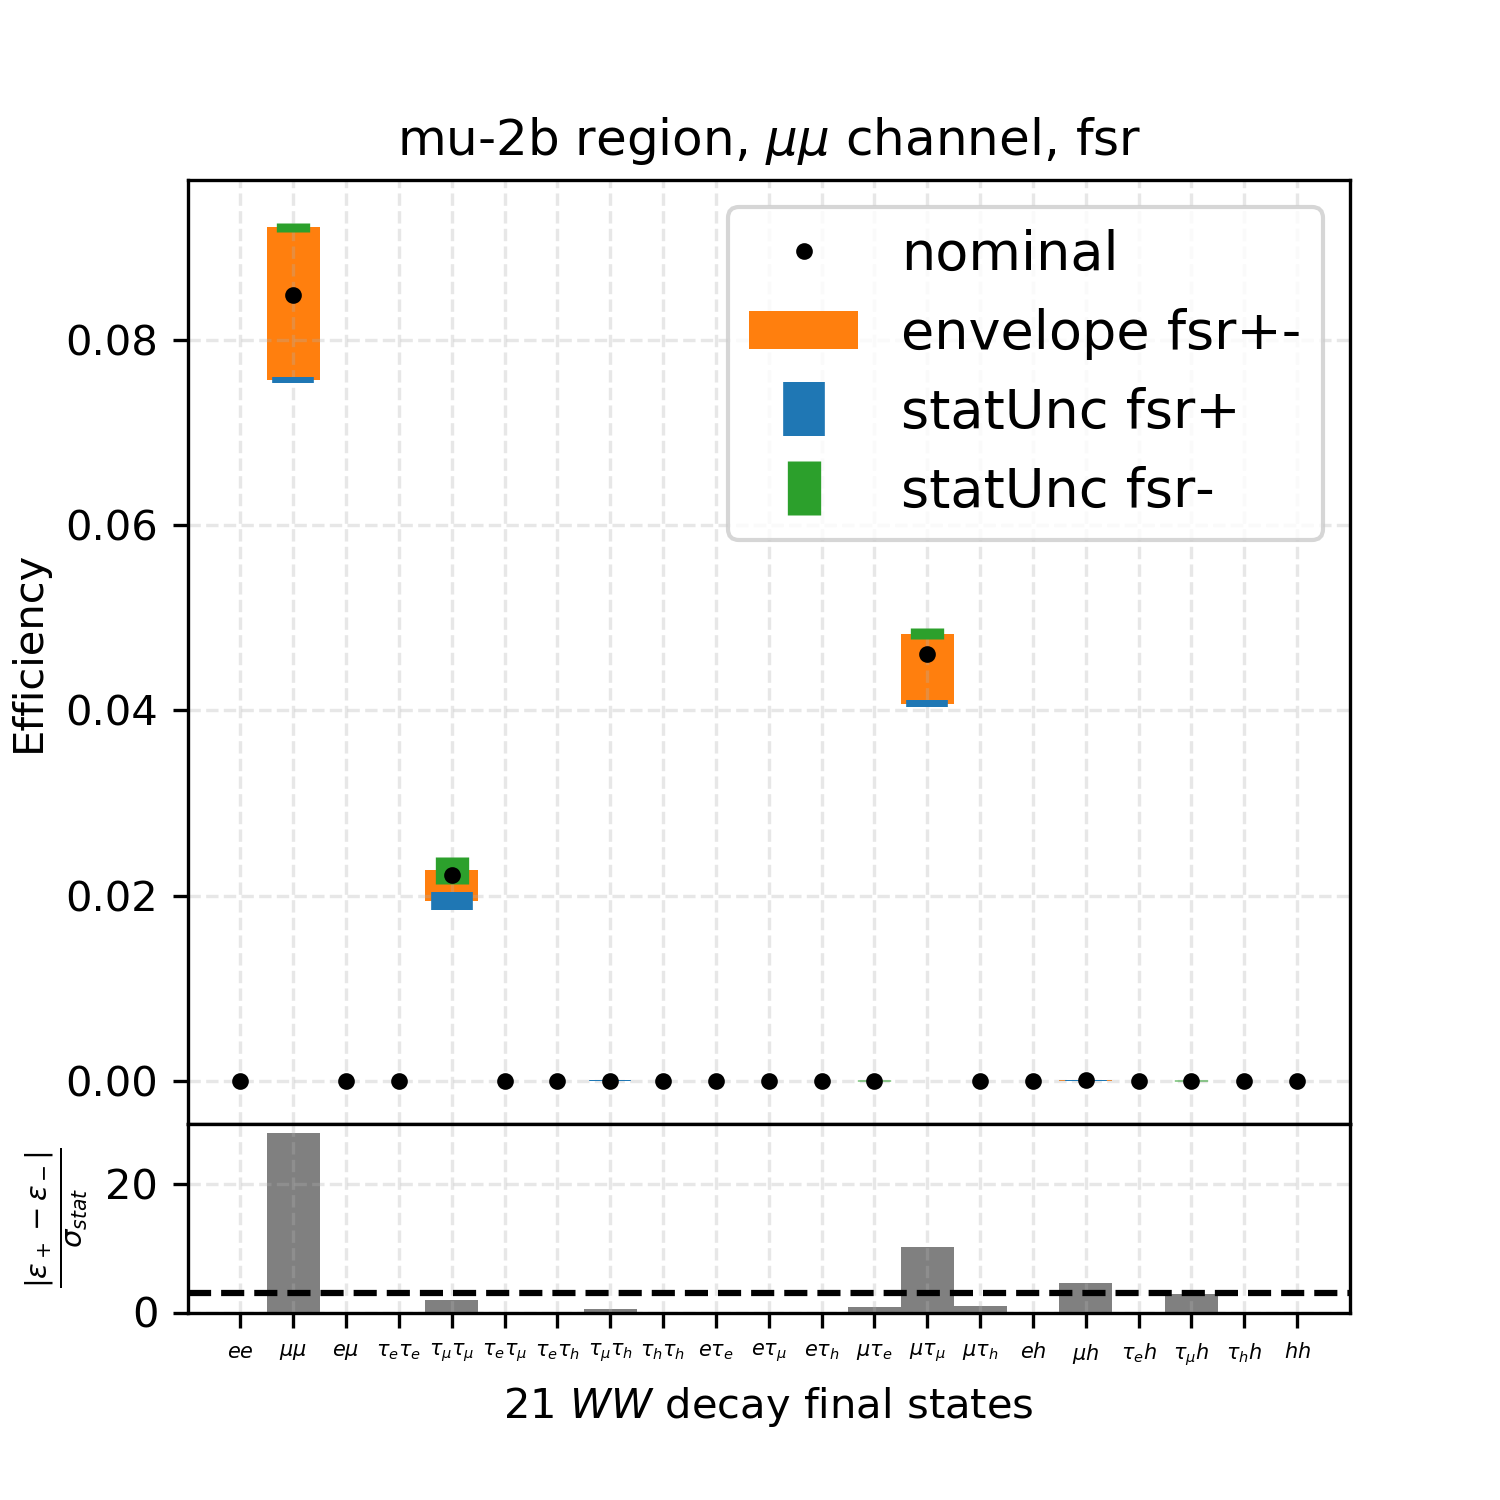
\includegraphics[width=0.24\textwidth]{chapters/Appendix/sectionTTSyst/figures/afterCorr/icata1_ch1_fsr.png}
    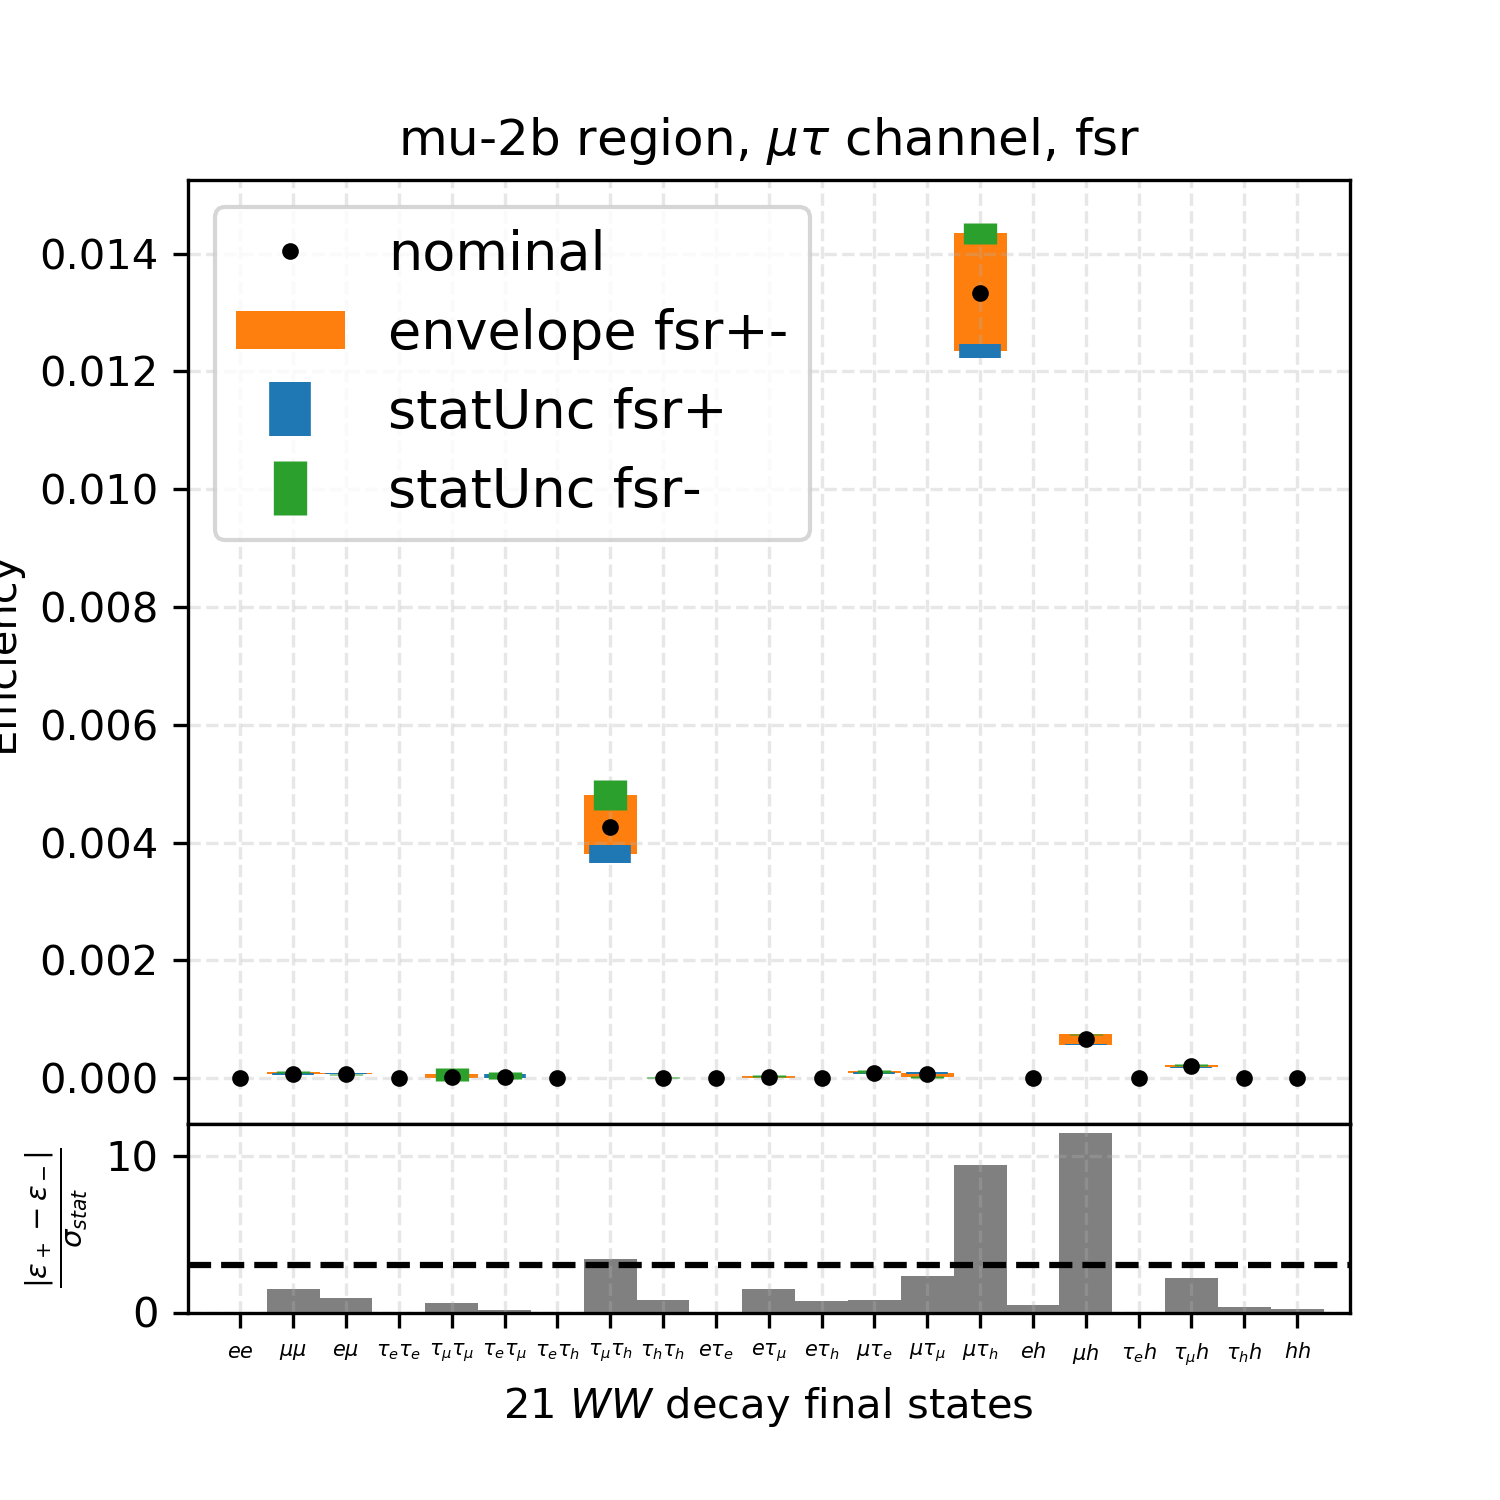
\includegraphics[width=0.24\textwidth]{chapters/Appendix/sectionTTSyst/figures/afterCorr/icata1_ch2_fsr.png}
    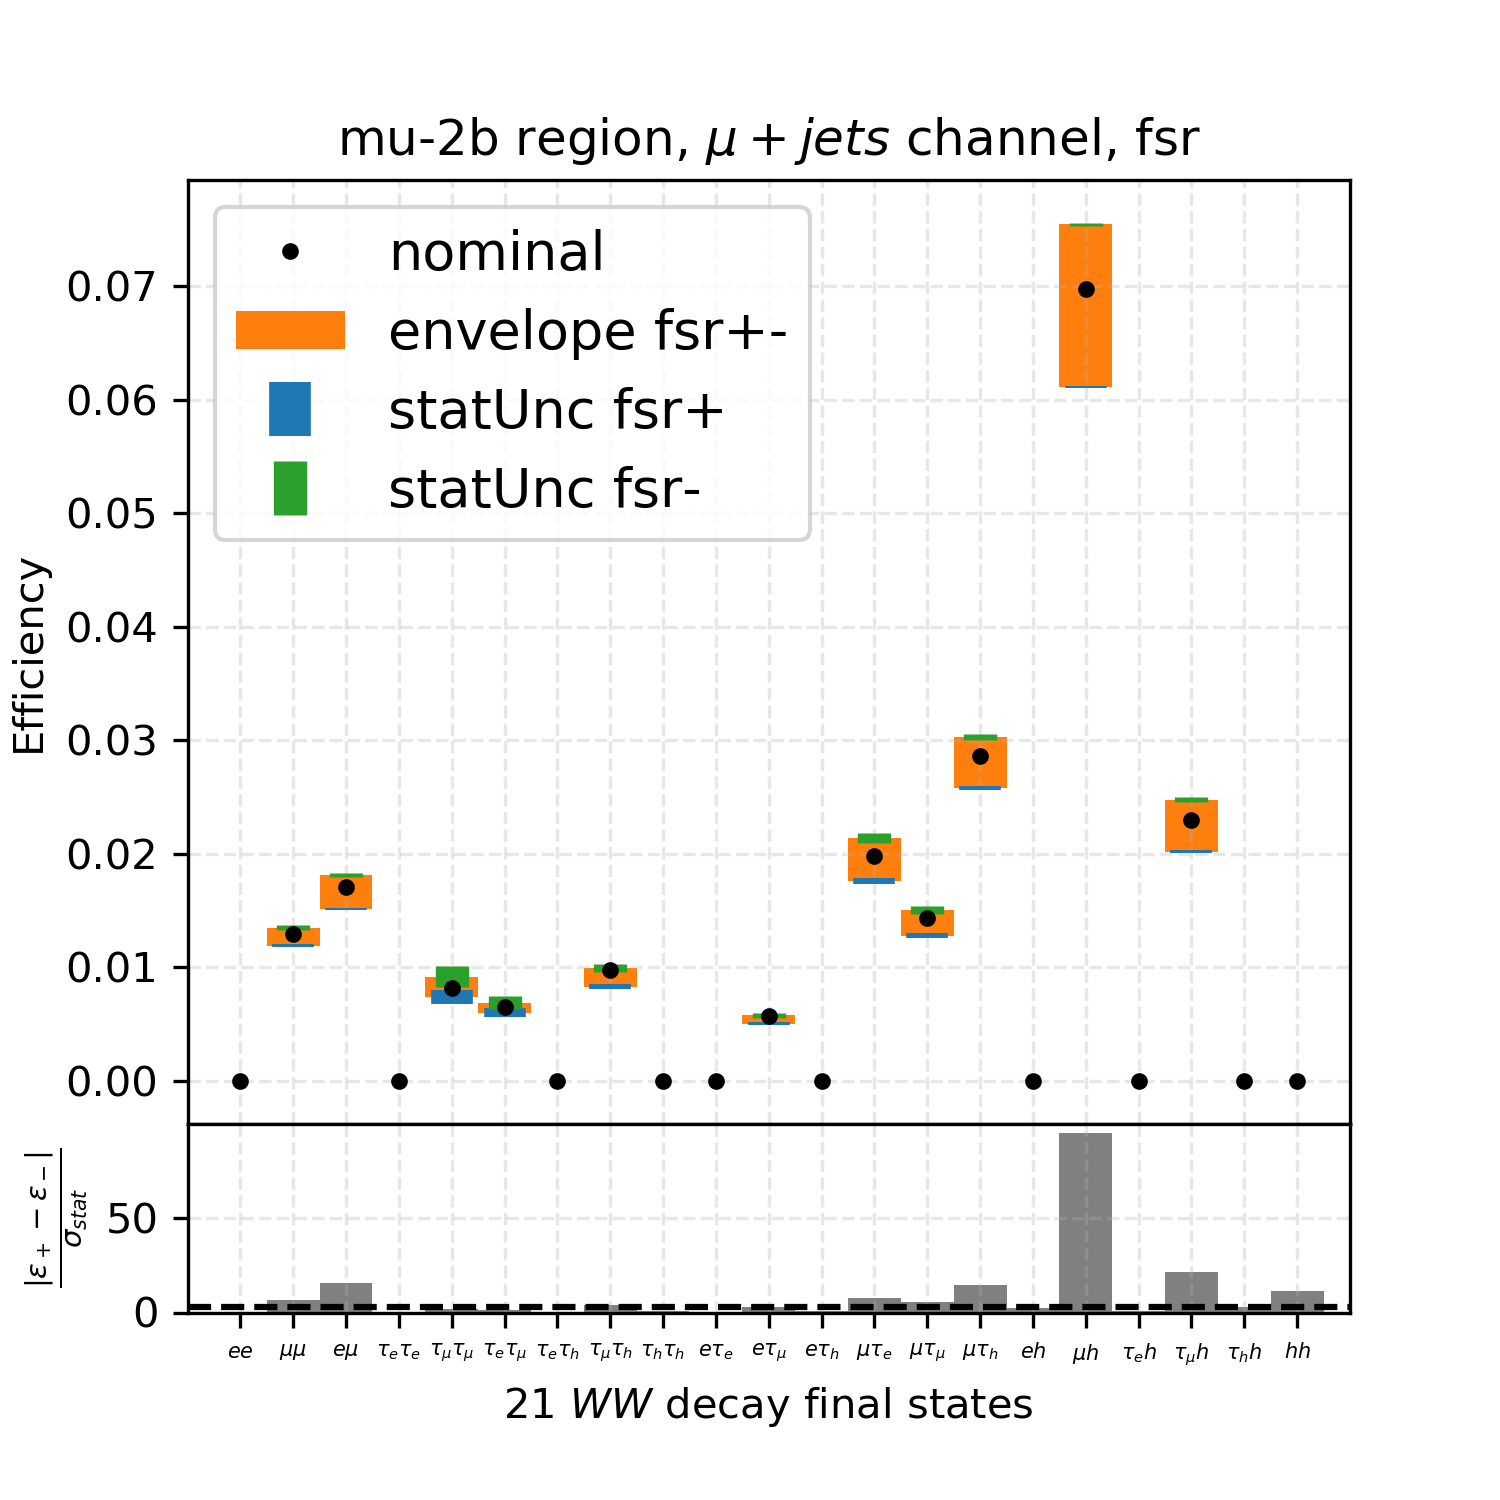
\includegraphics[width=0.24\textwidth]{chapters/Appendix/sectionTTSyst/figures/afterCorr/icata1_ch3_fsr.png}
    
    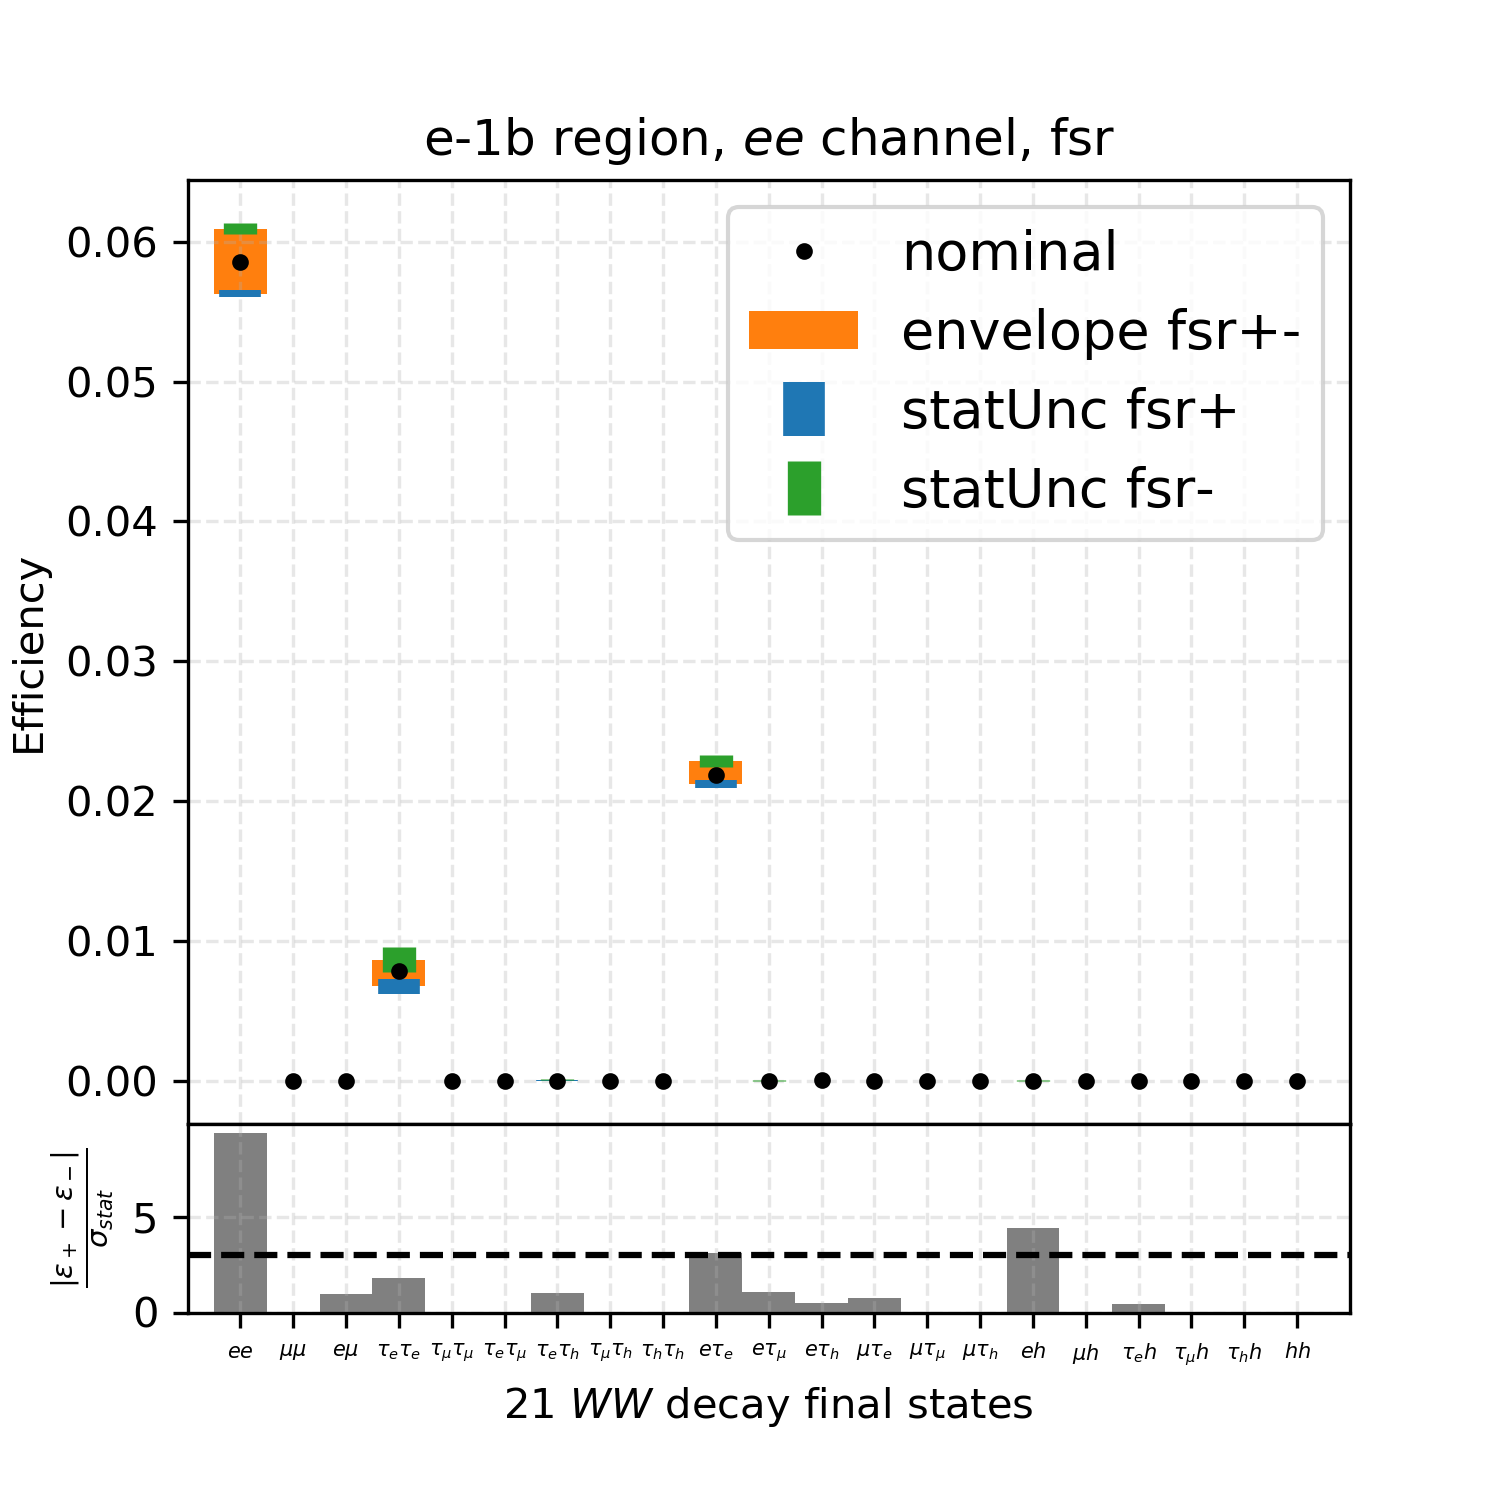
\includegraphics[width=0.24\textwidth]{chapters/Appendix/sectionTTSyst/figures/afterCorr/icata2_ch0_fsr.png}
    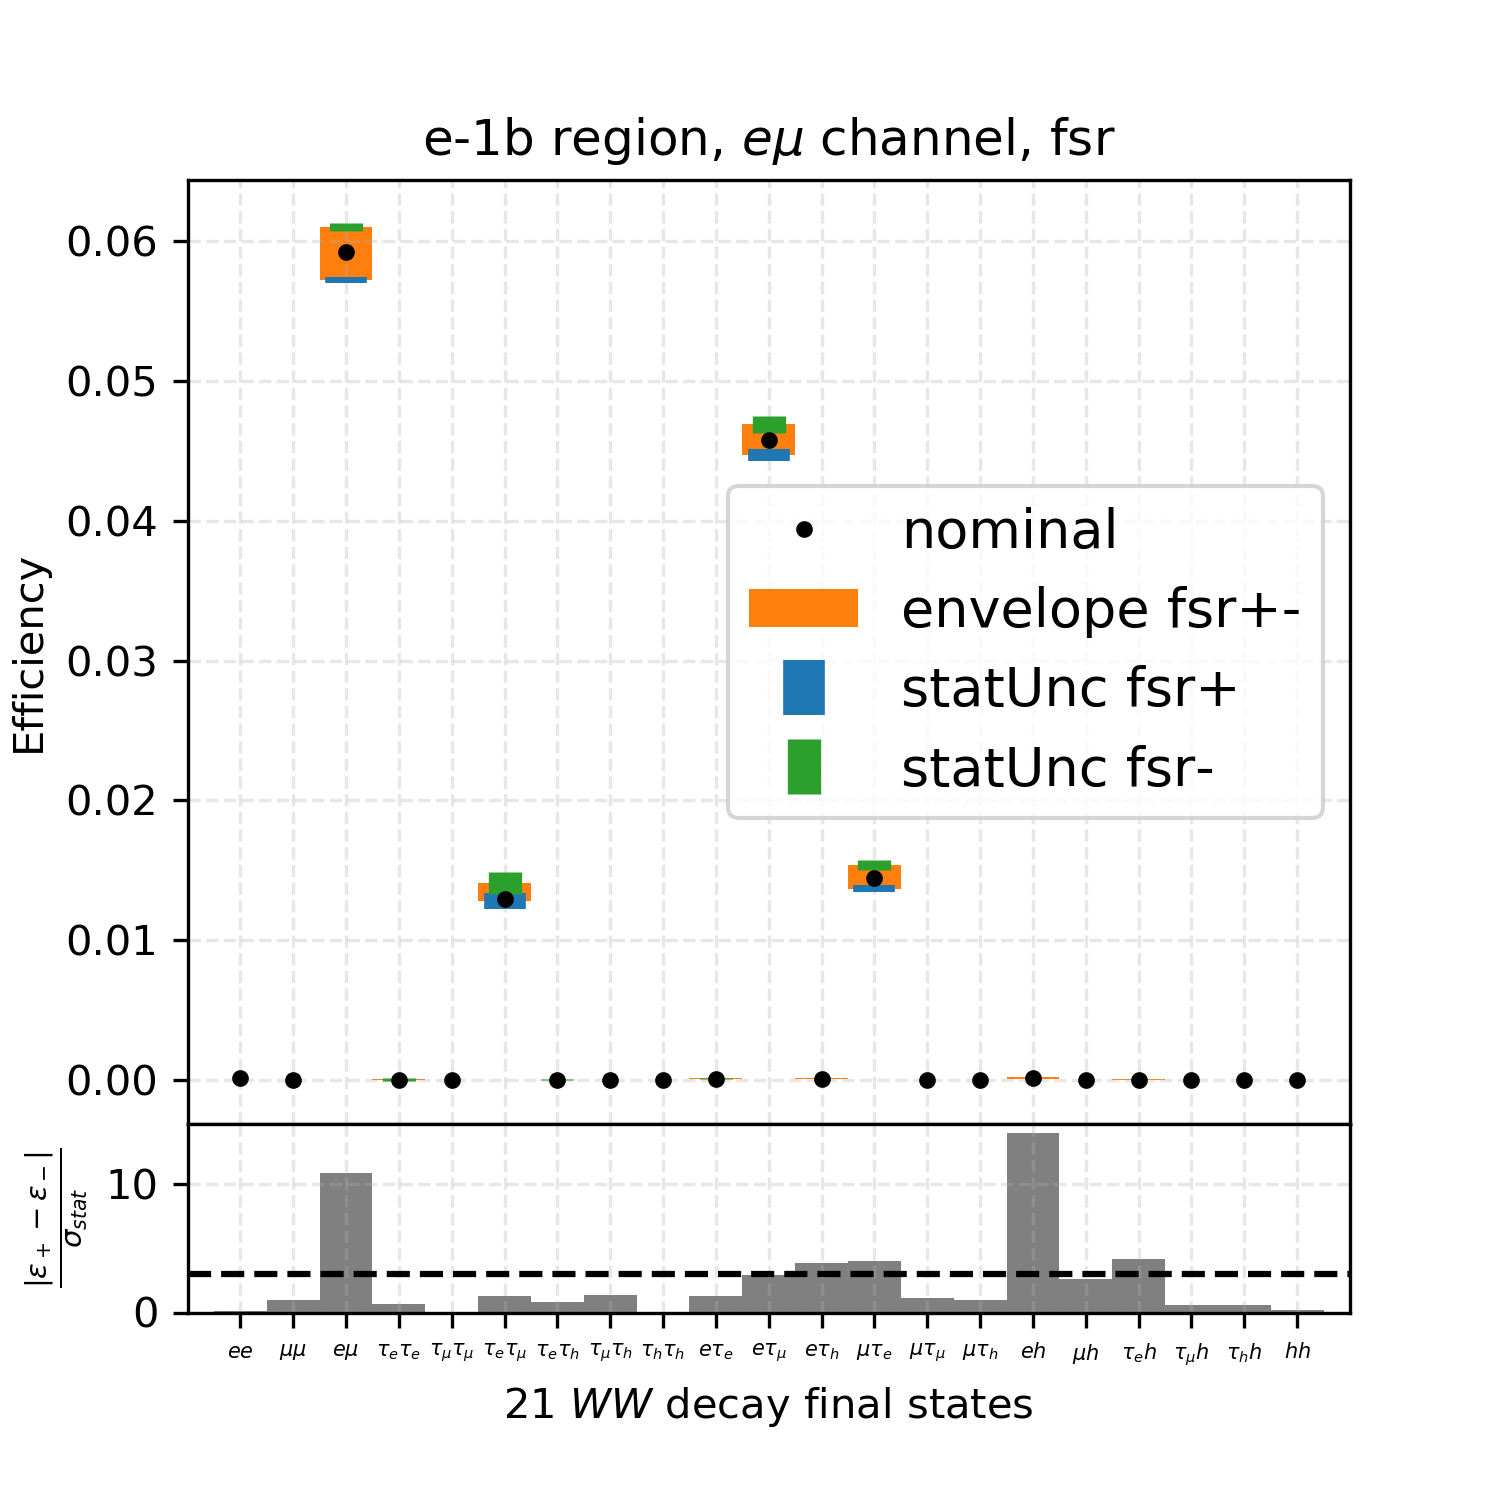
\includegraphics[width=0.24\textwidth]{chapters/Appendix/sectionTTSyst/figures/afterCorr/icata2_ch1_fsr.png}
    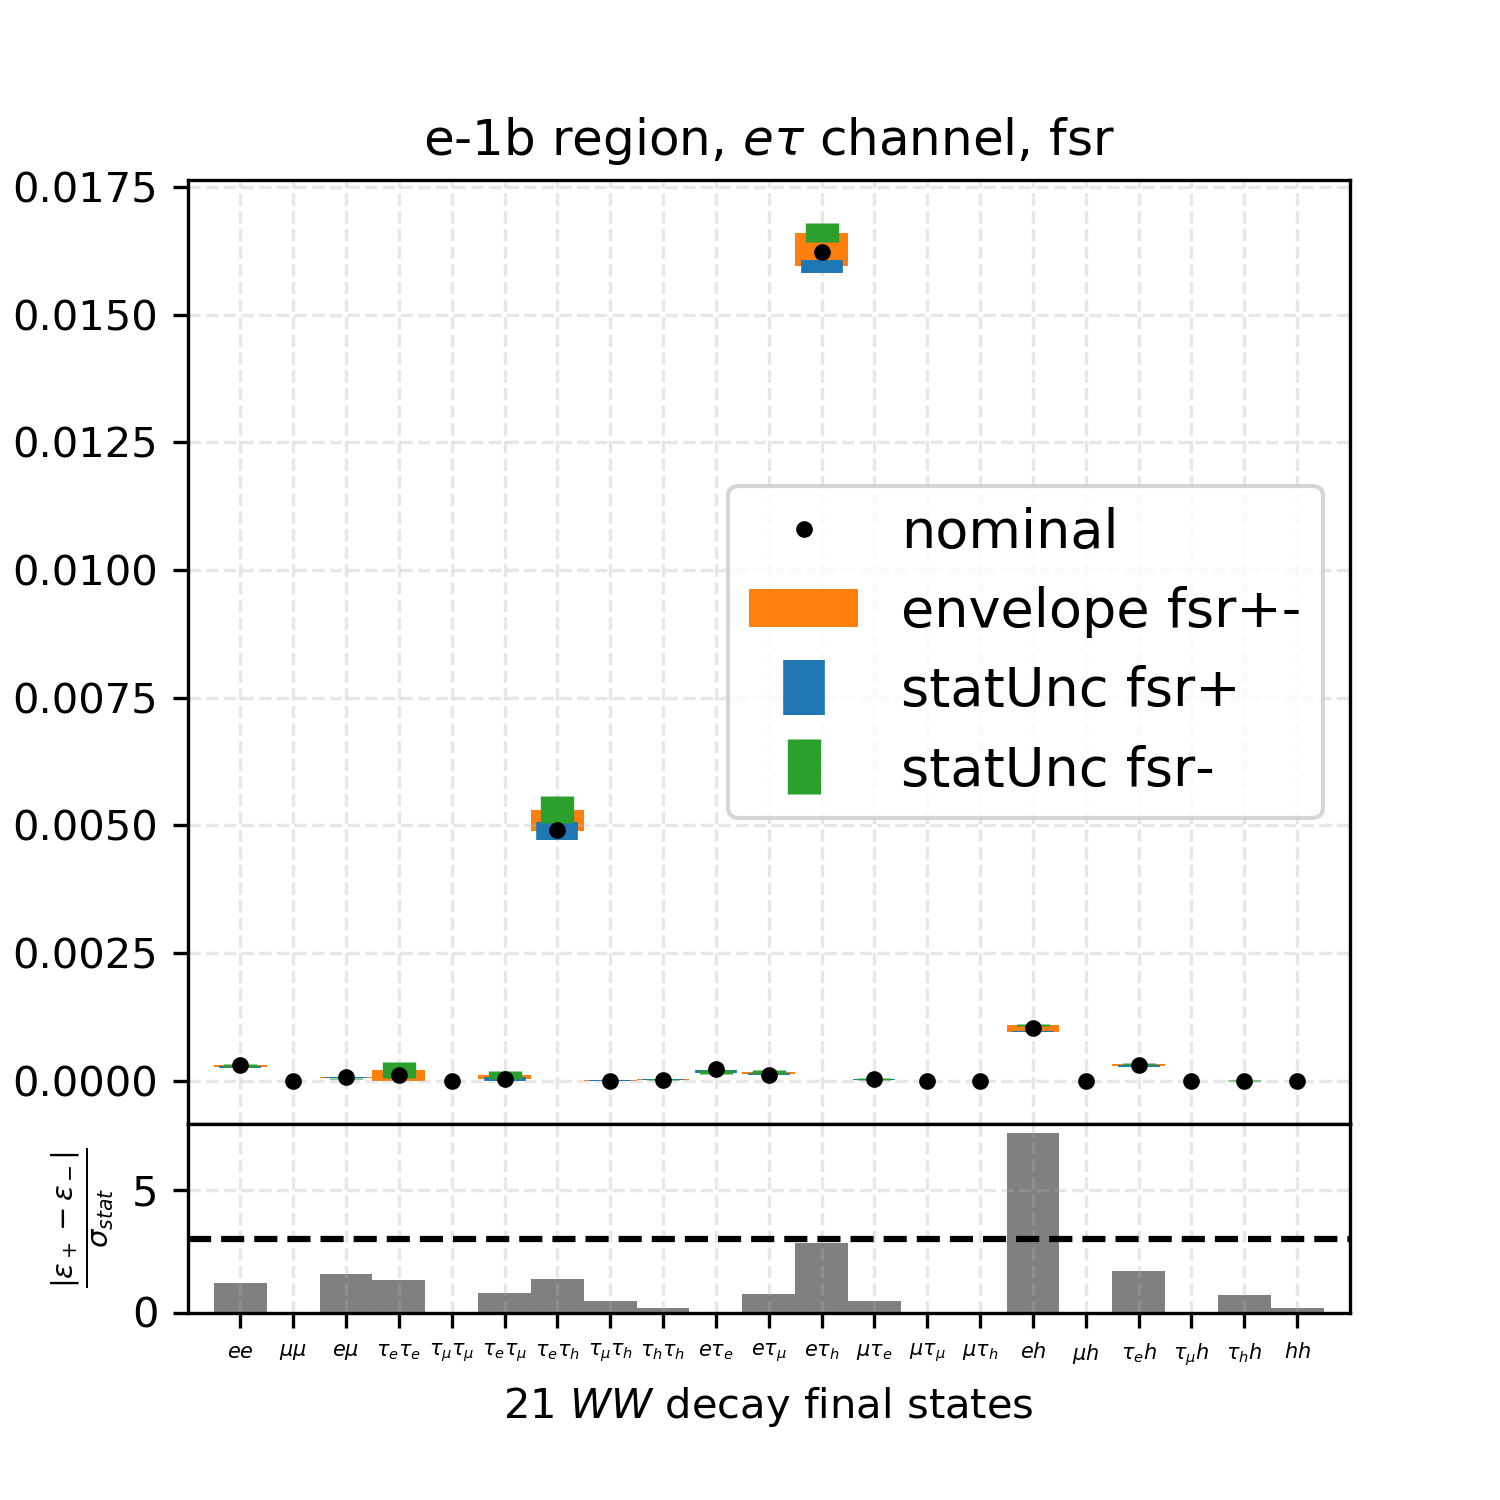
\includegraphics[width=0.24\textwidth]{chapters/Appendix/sectionTTSyst/figures/afterCorr/icata2_ch2_fsr.png}
    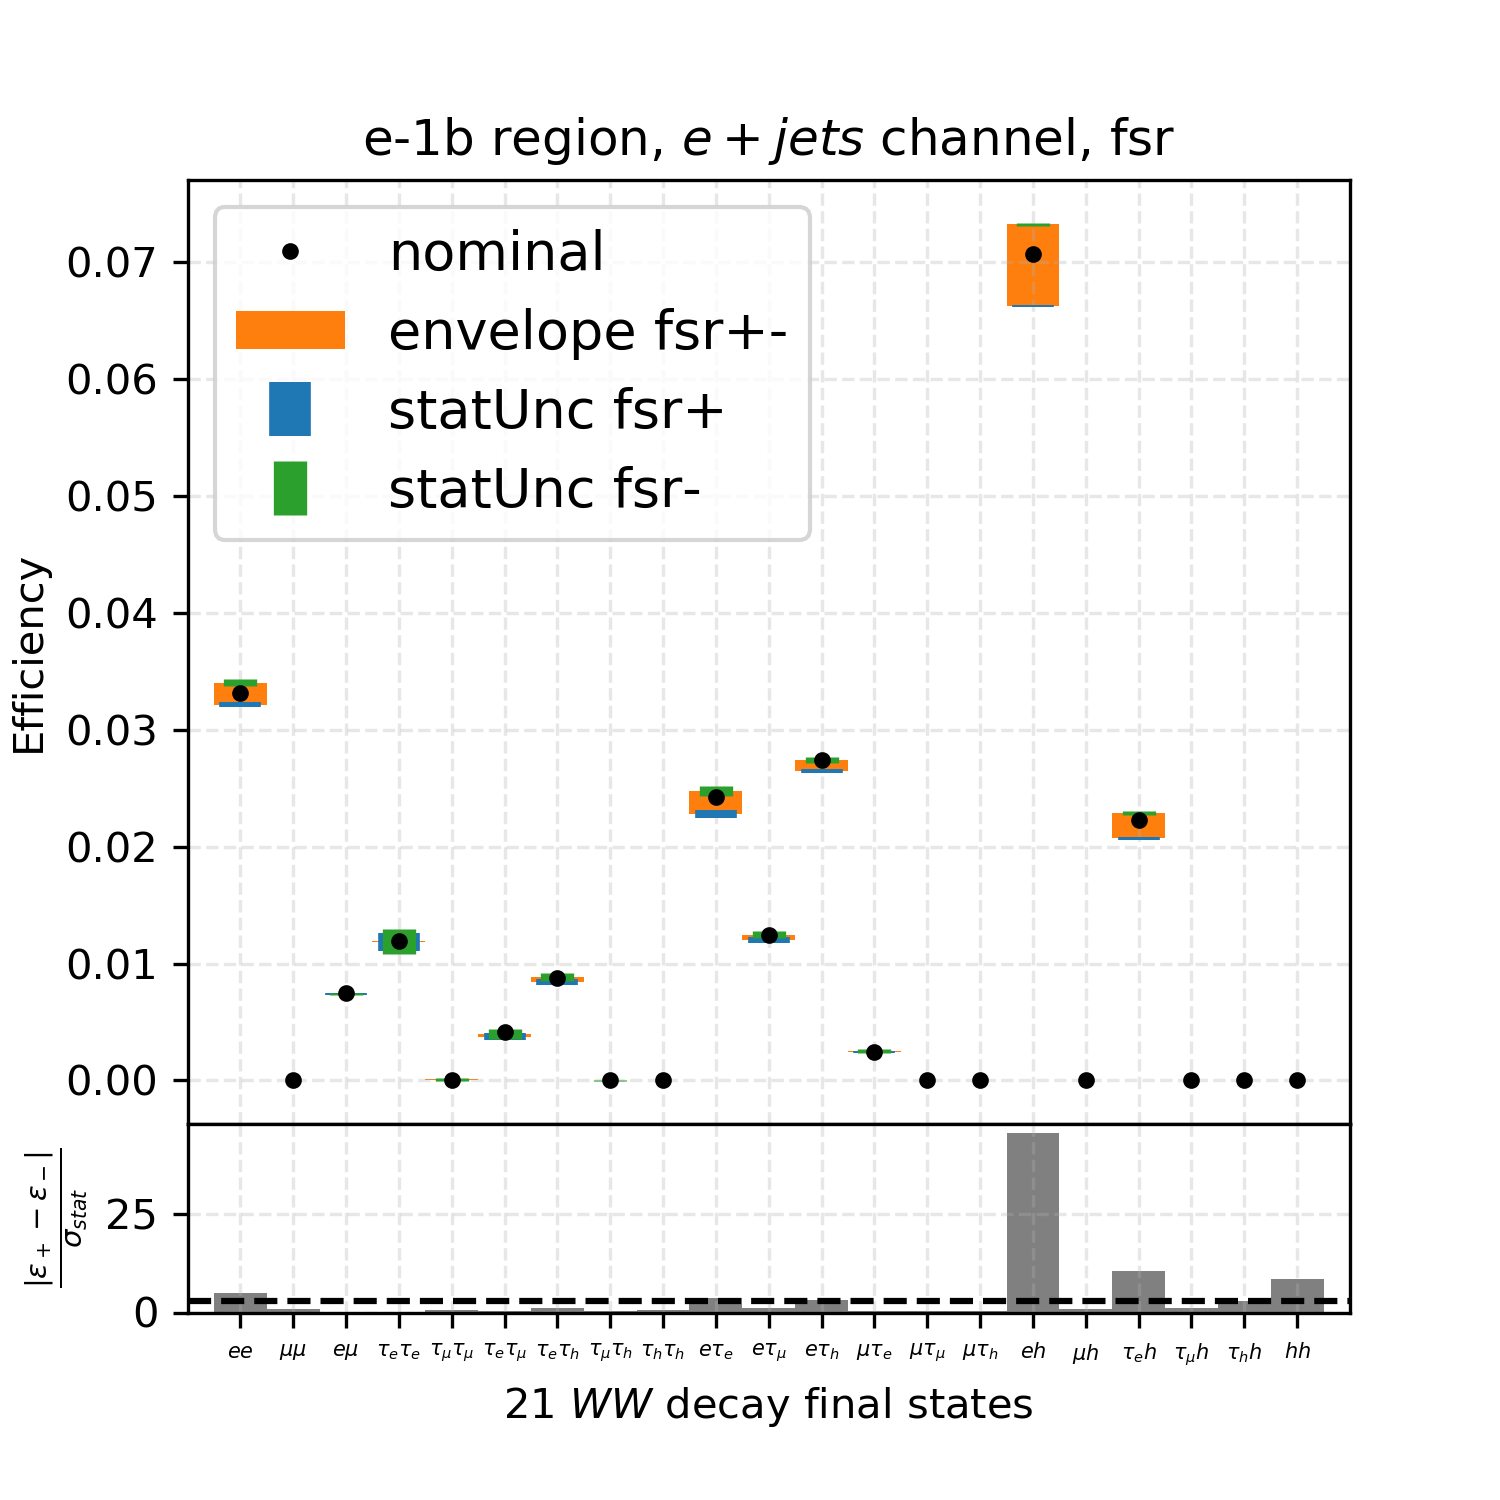
\includegraphics[width=0.24\textwidth]{chapters/Appendix/sectionTTSyst/figures/afterCorr/icata2_ch3_fsr.png}

    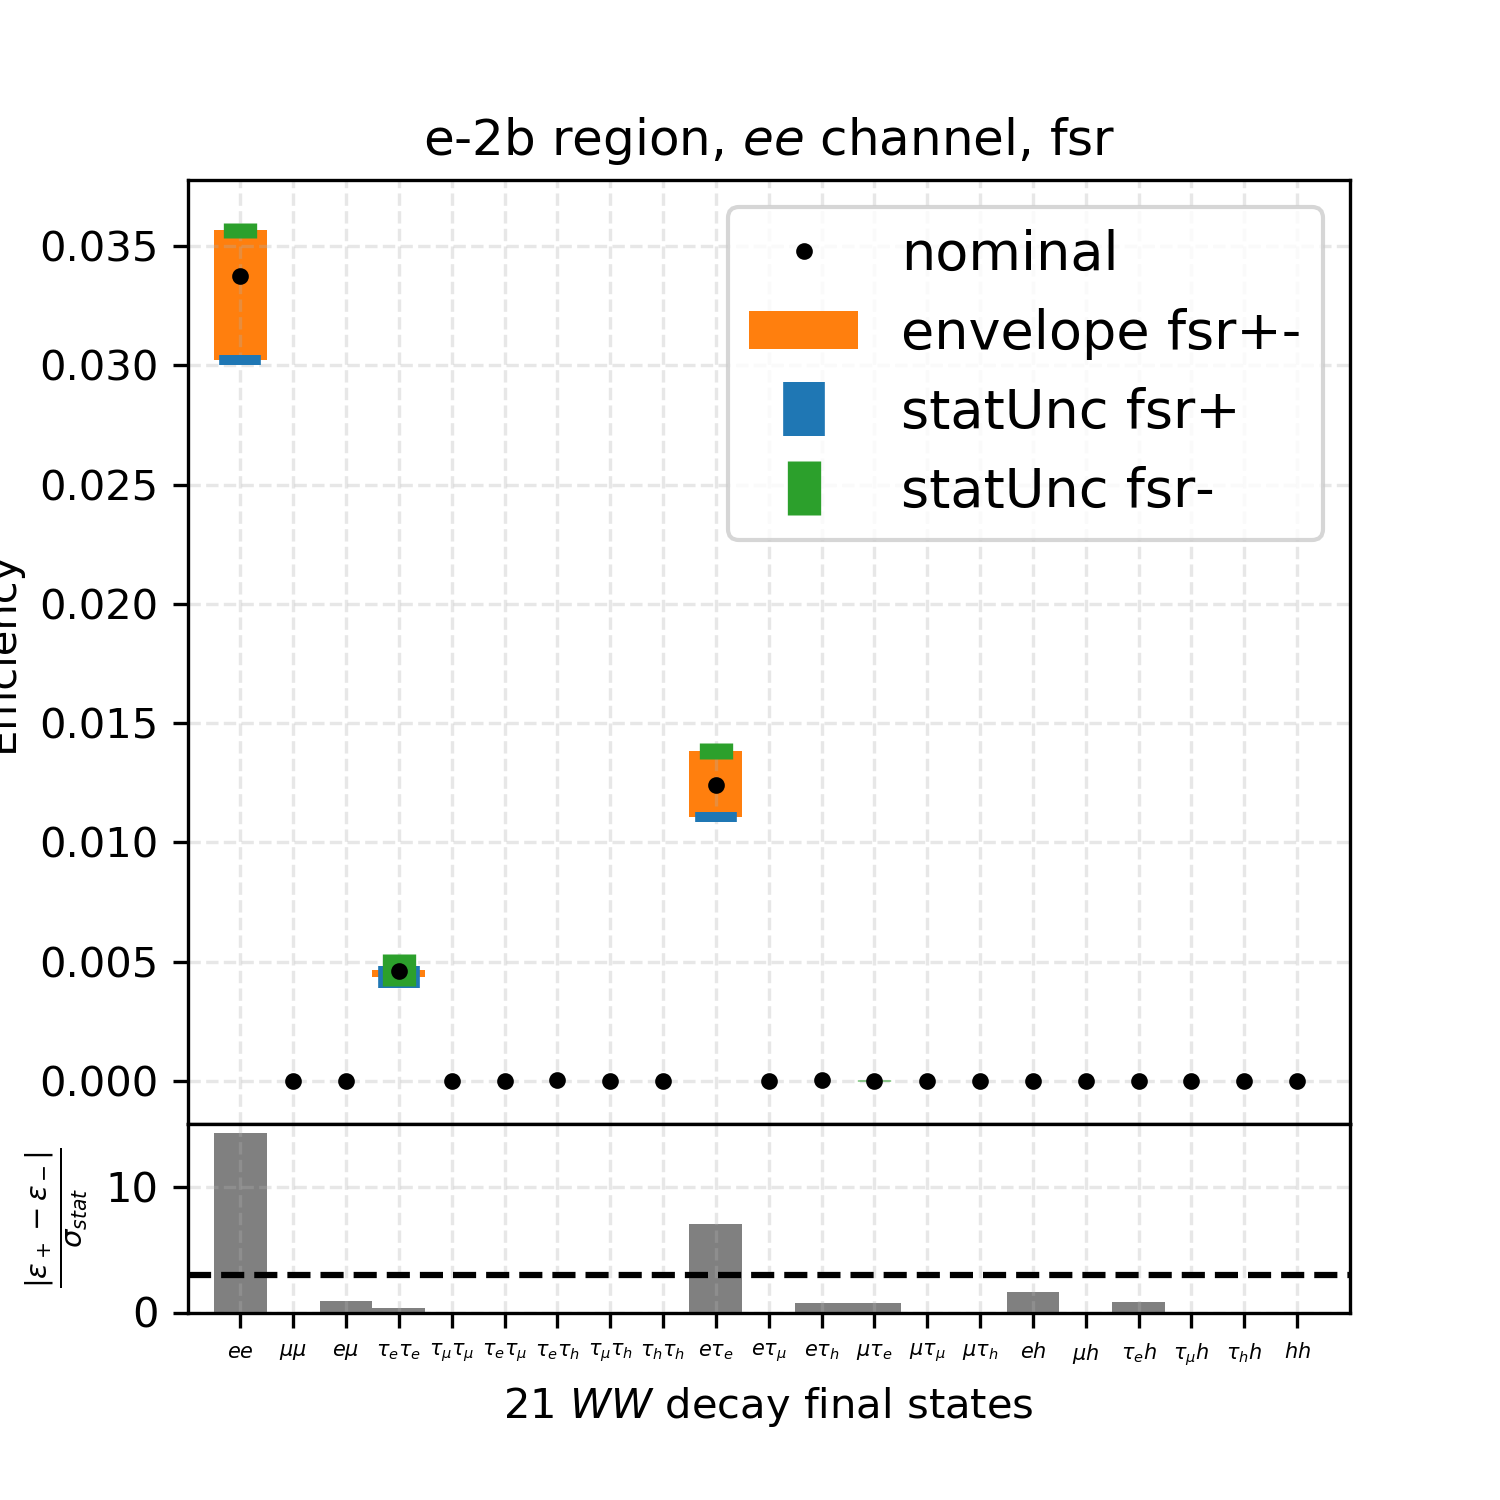
\includegraphics[width=0.24\textwidth]{chapters/Appendix/sectionTTSyst/figures/afterCorr/icata3_ch0_fsr.png}
    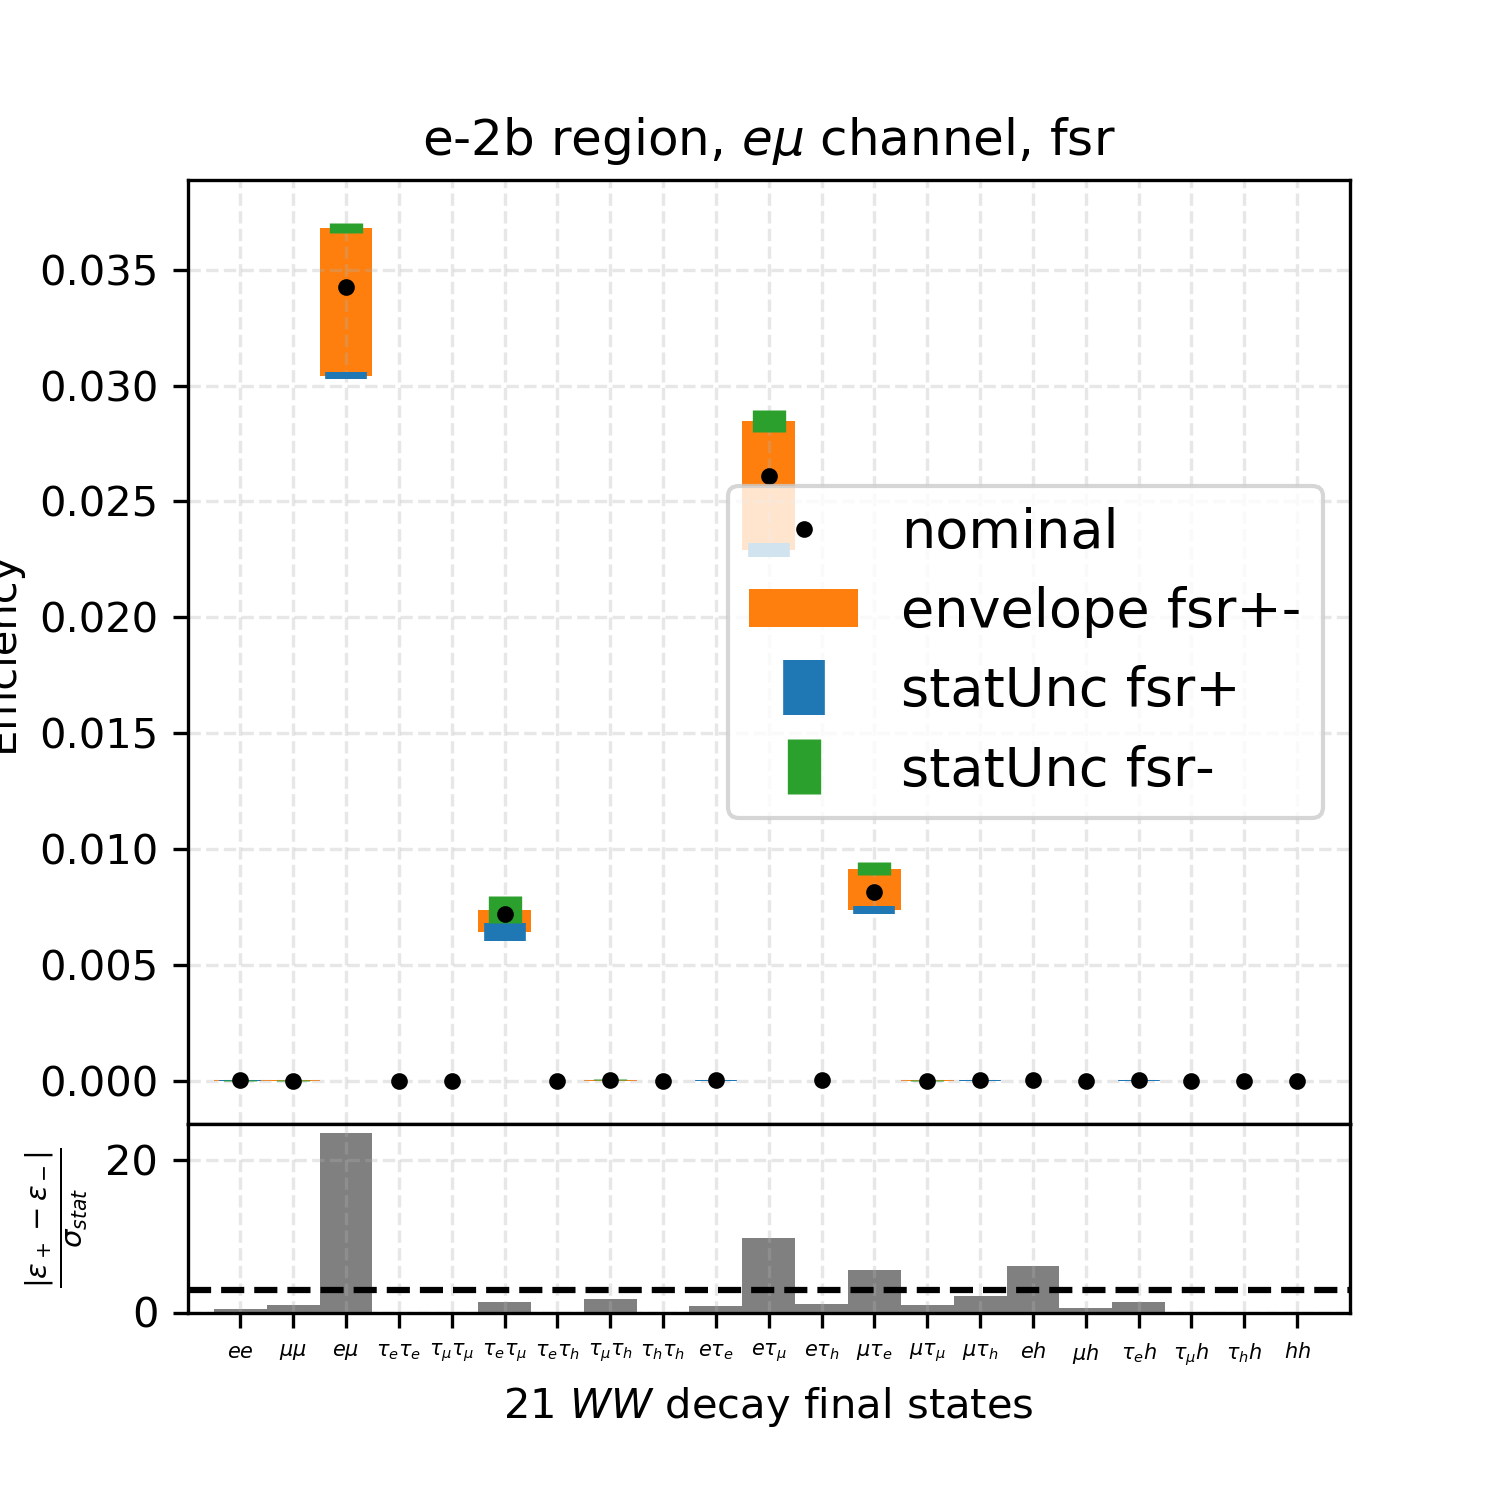
\includegraphics[width=0.24\textwidth]{chapters/Appendix/sectionTTSyst/figures/afterCorr/icata3_ch1_fsr.png}
    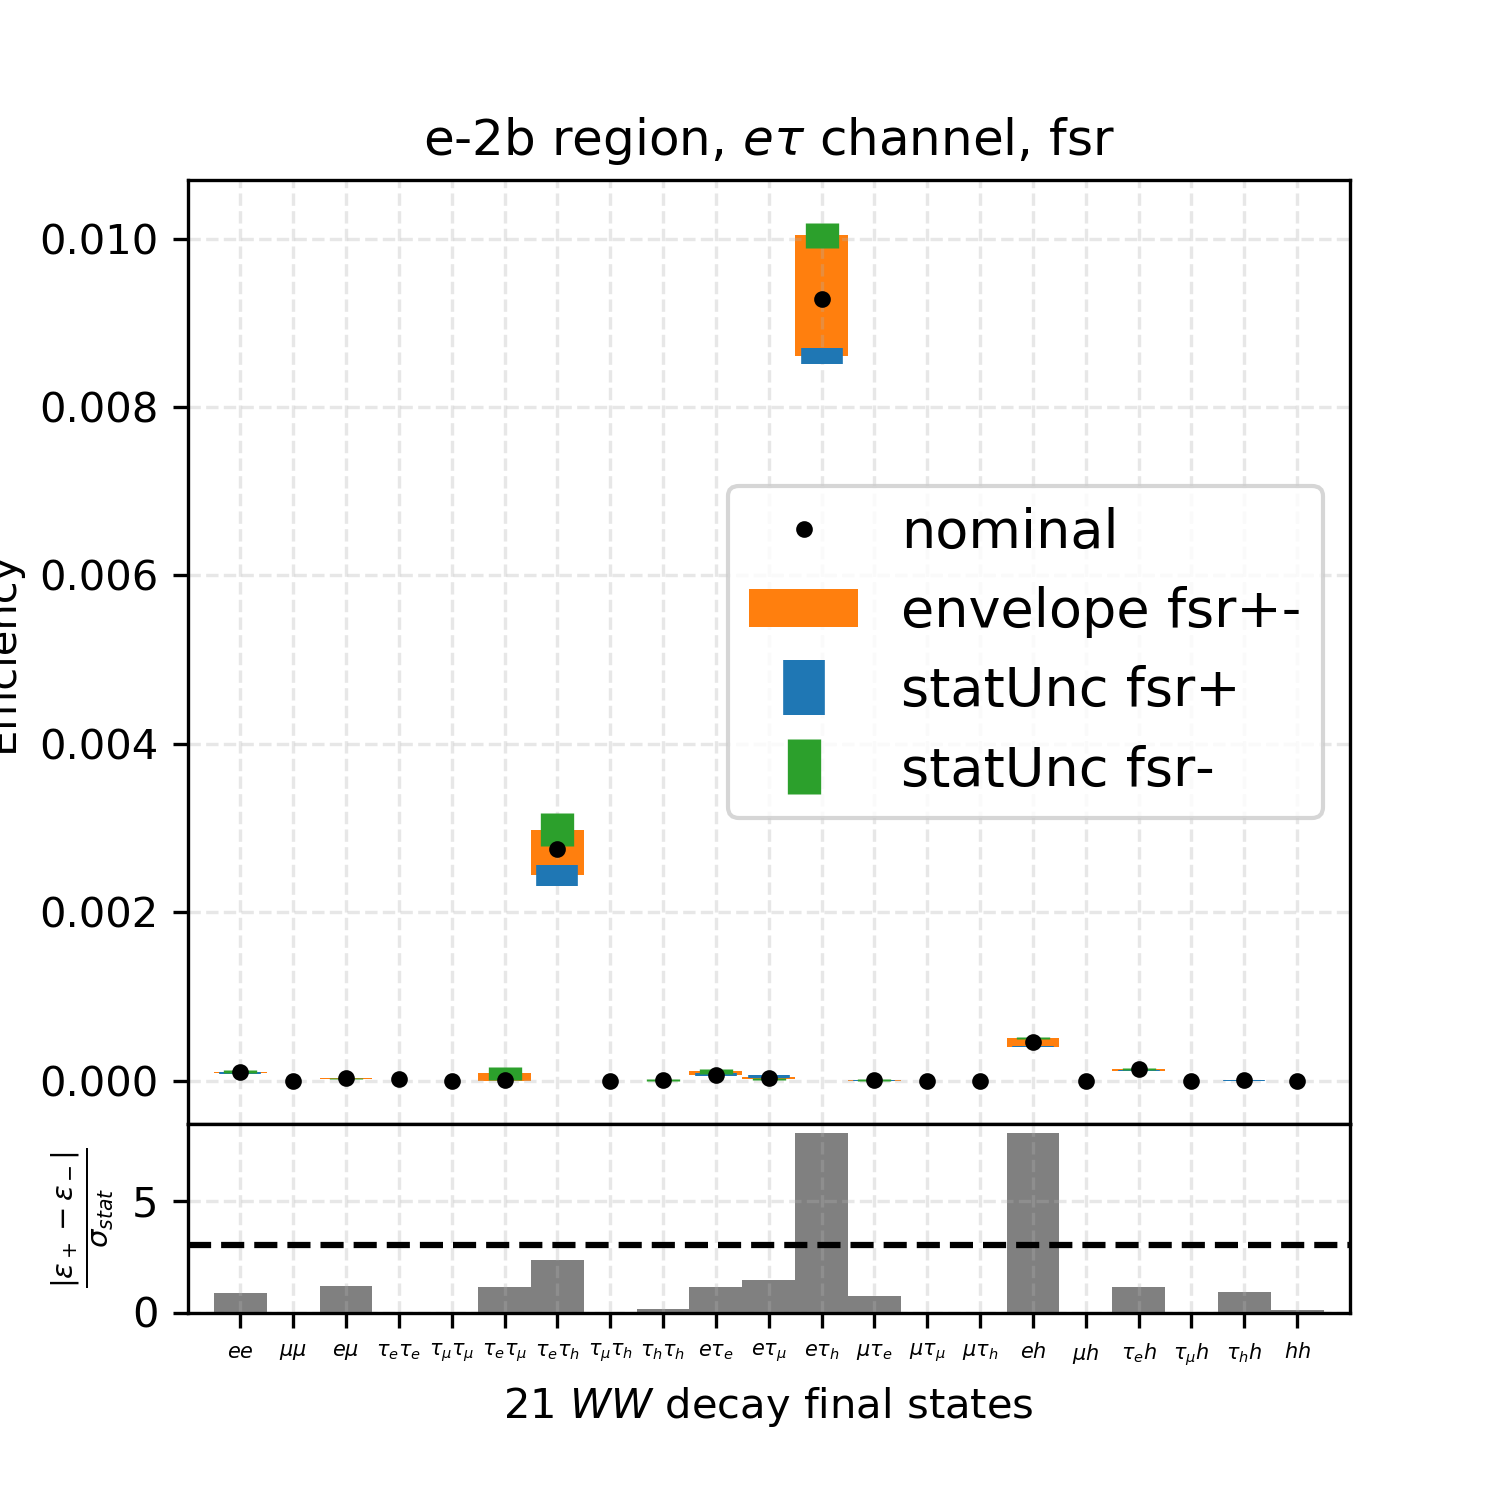
\includegraphics[width=0.24\textwidth]{chapters/Appendix/sectionTTSyst/figures/afterCorr/icata3_ch2_fsr.png}
    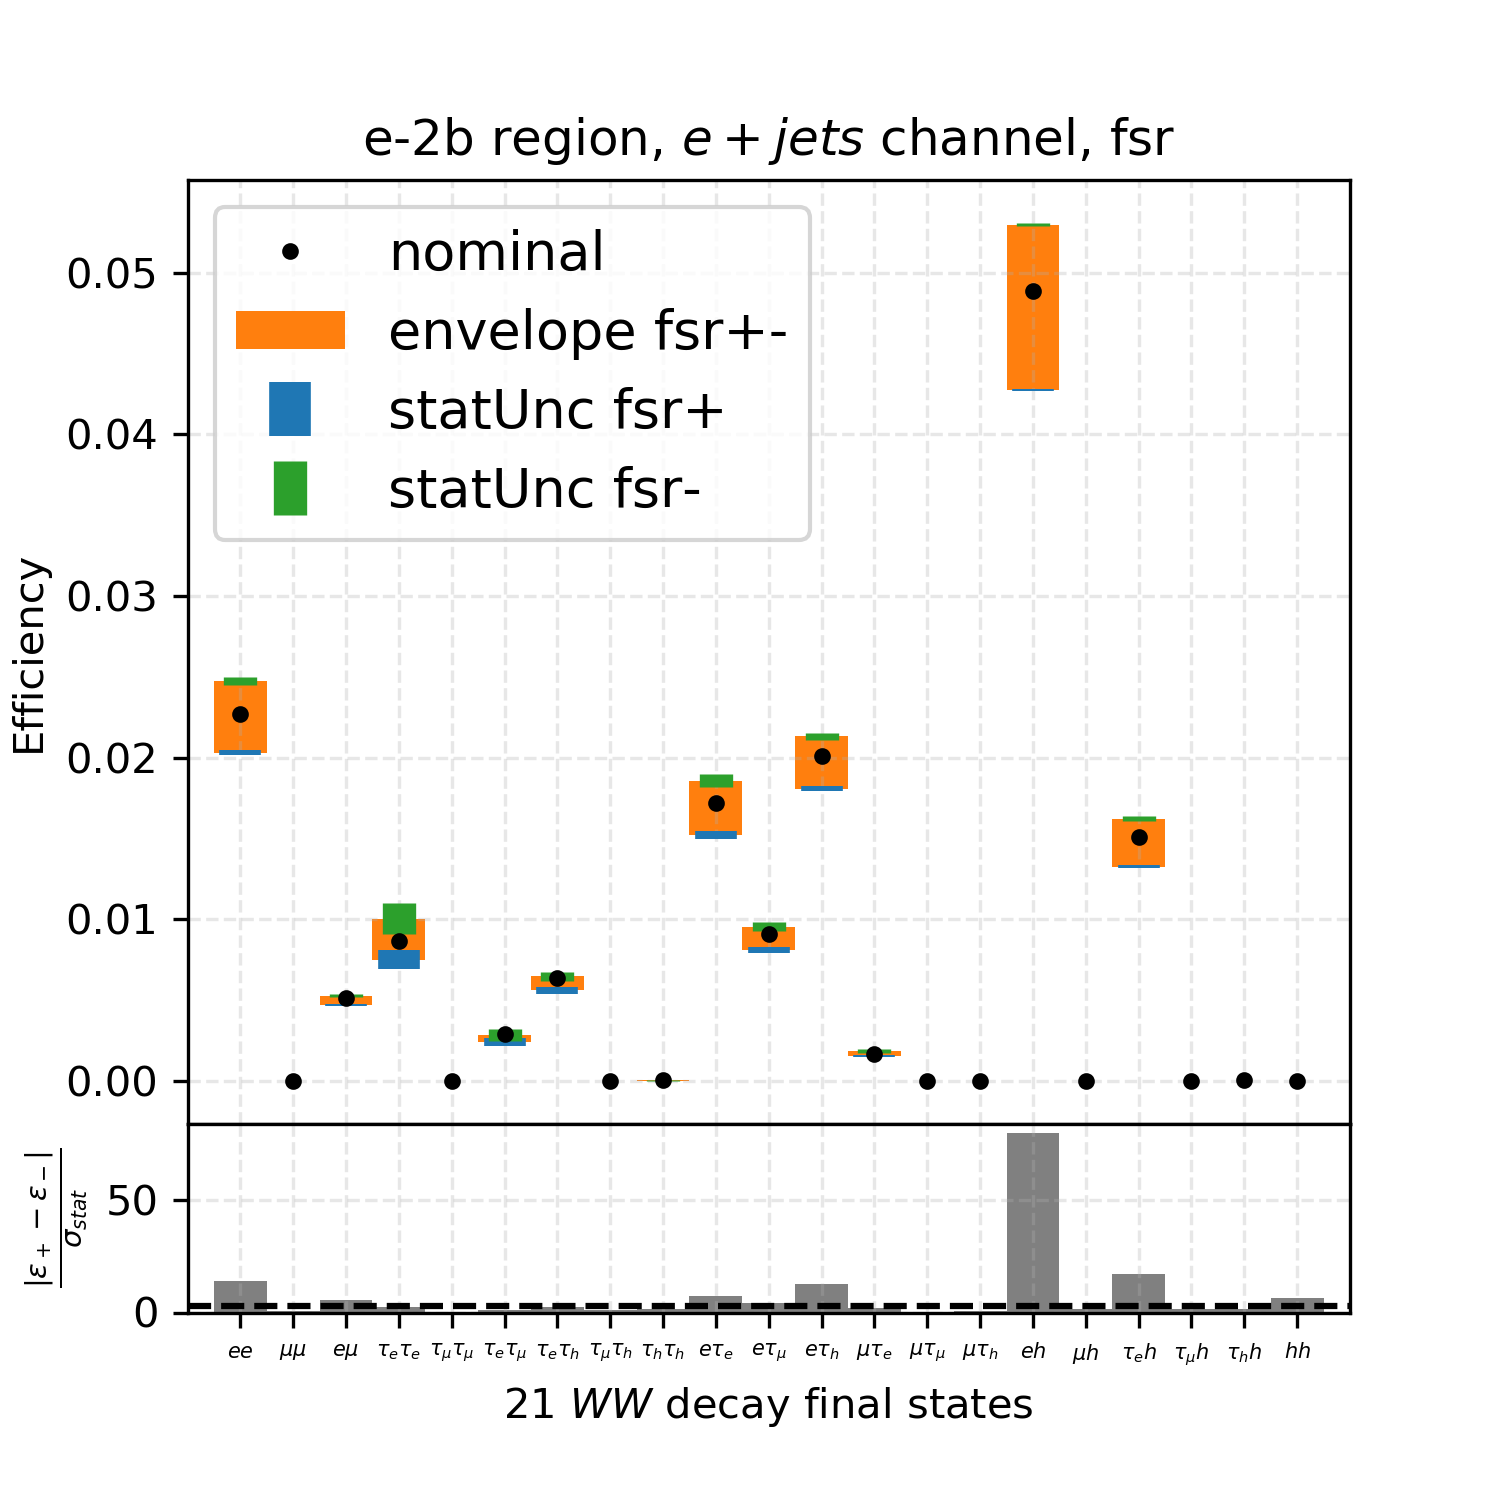
\includegraphics[width=0.24\textwidth]{chapters/Appendix/sectionTTSyst/figures/afterCorr/icata3_ch3_fsr.png}
    
    \caption{Reweight $\tau_h$ and $j \to \tau_h$ efficiencies in the dedicated FSR, ISF, MEPS, UE ttbar samples}
    \label{fig:appendix:reweighttt:effAfterCorrFSR}
\end{figure}



\begin{figure}
    \centering
    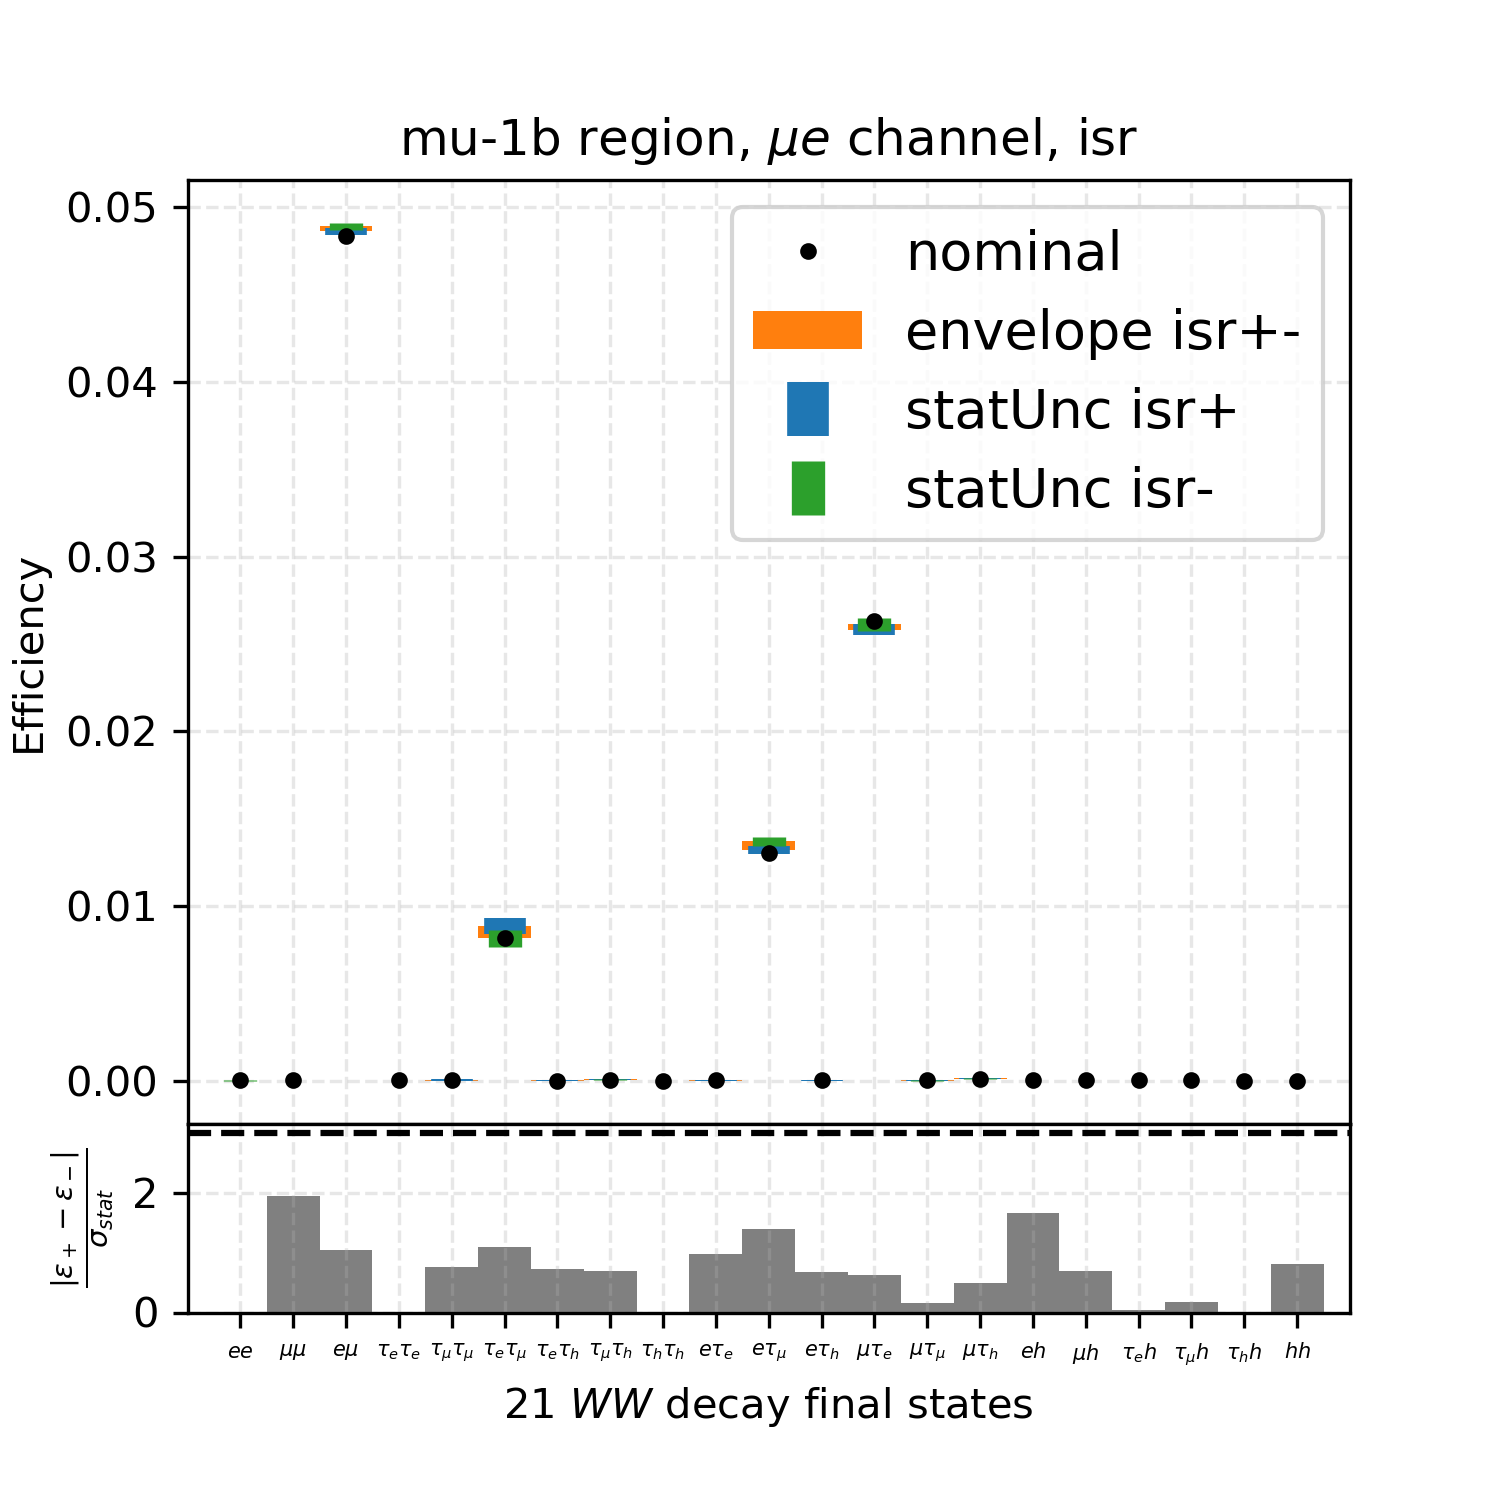
\includegraphics[width=0.24\textwidth]{chapters/Appendix/sectionTTSyst/figures/afterCorr/icata0_ch0_isr.png}
    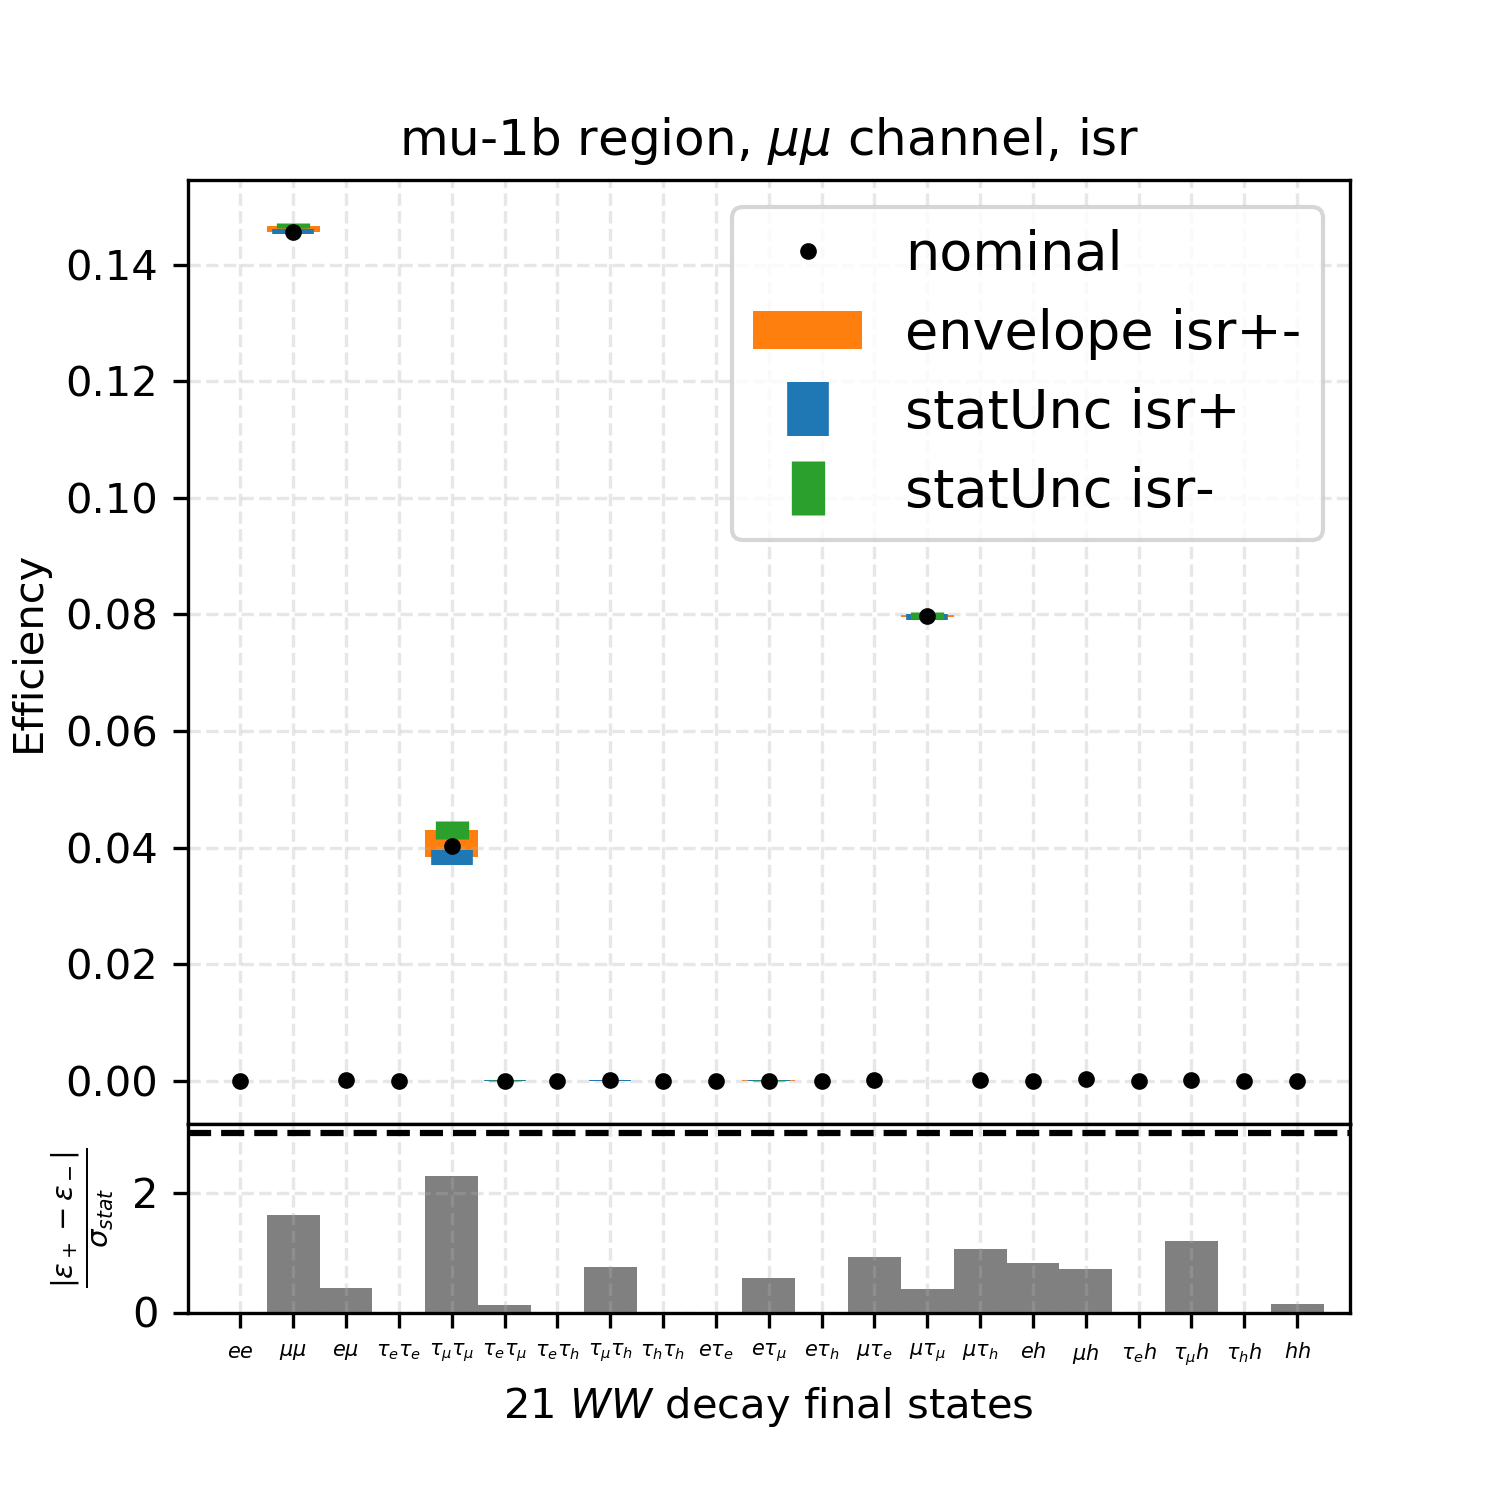
\includegraphics[width=0.24\textwidth]{chapters/Appendix/sectionTTSyst/figures/afterCorr/icata0_ch1_isr.png}
    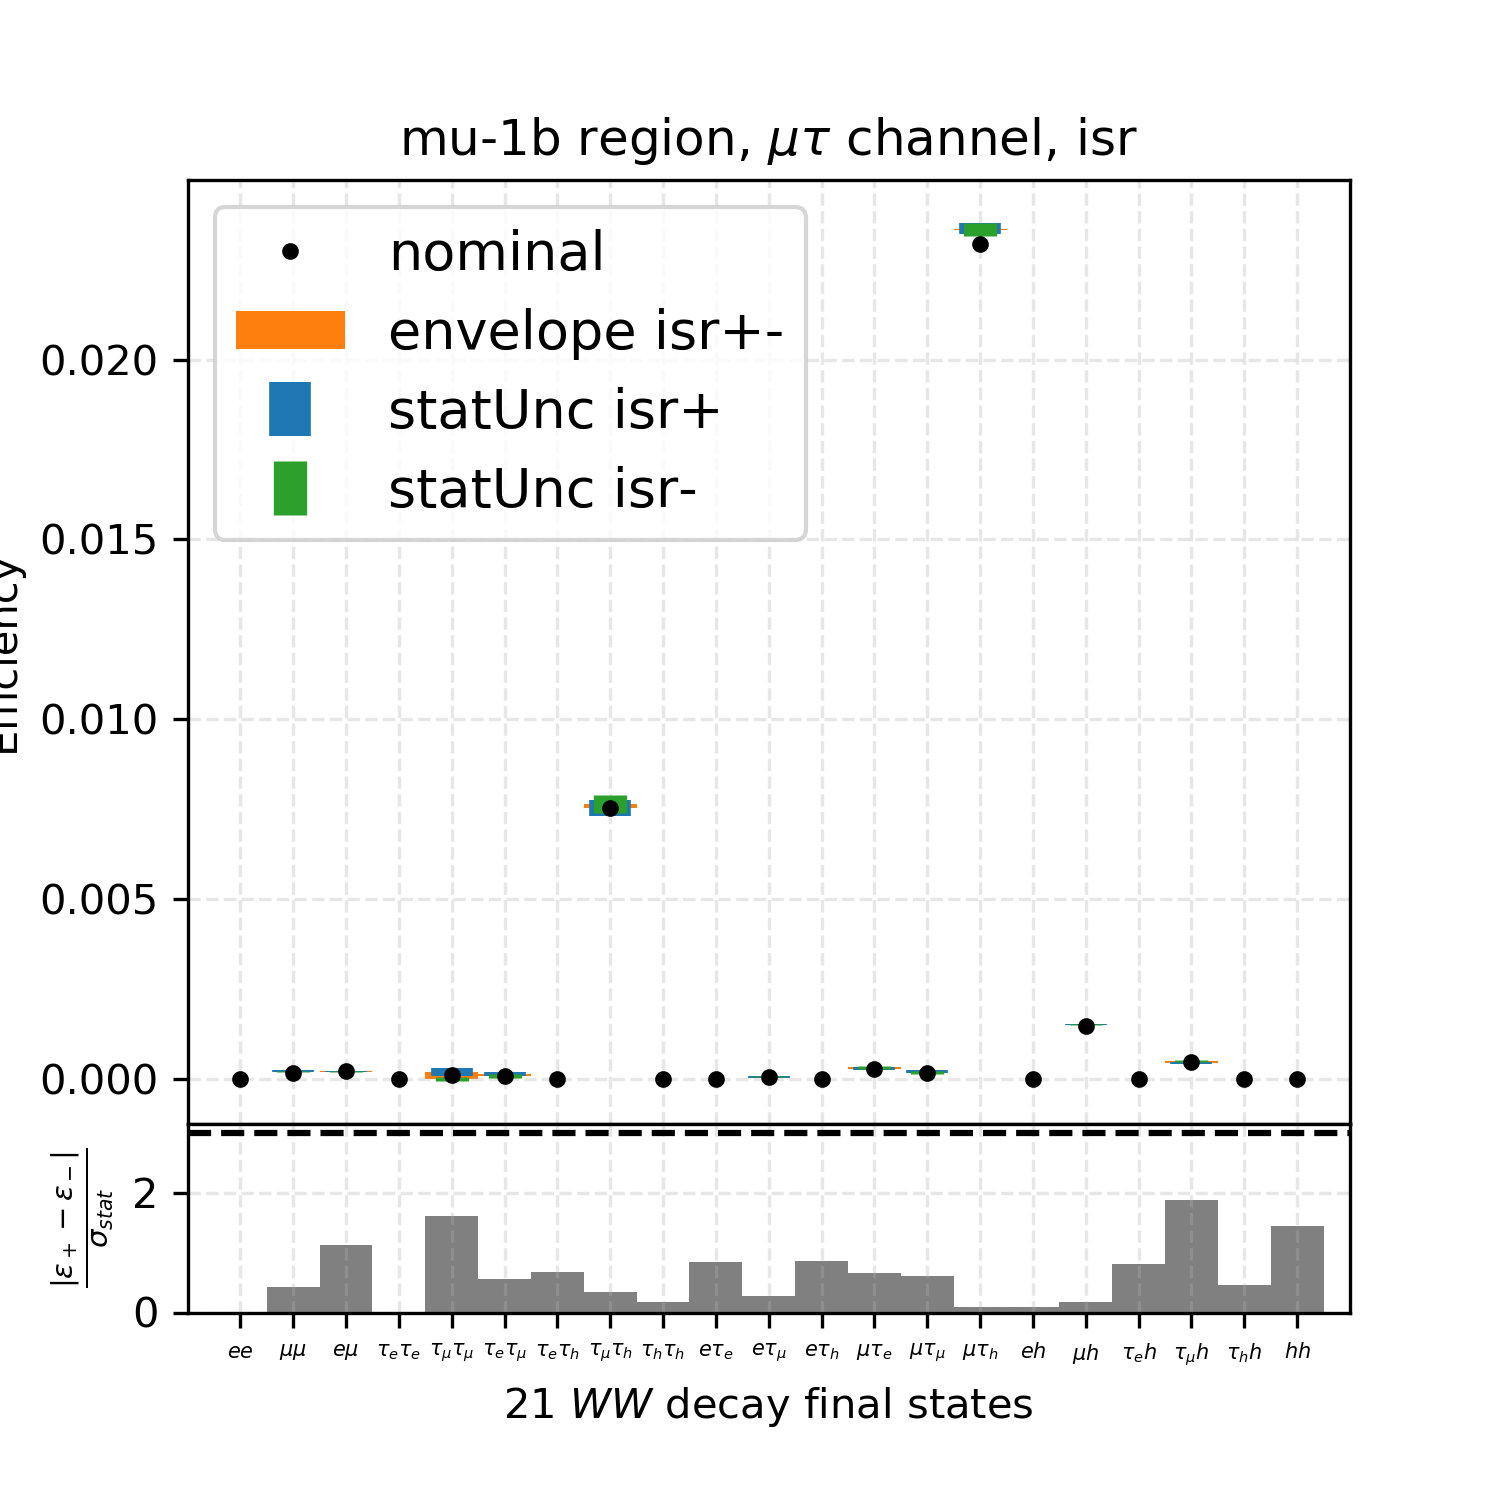
\includegraphics[width=0.24\textwidth]{chapters/Appendix/sectionTTSyst/figures/afterCorr/icata0_ch2_isr.png}
    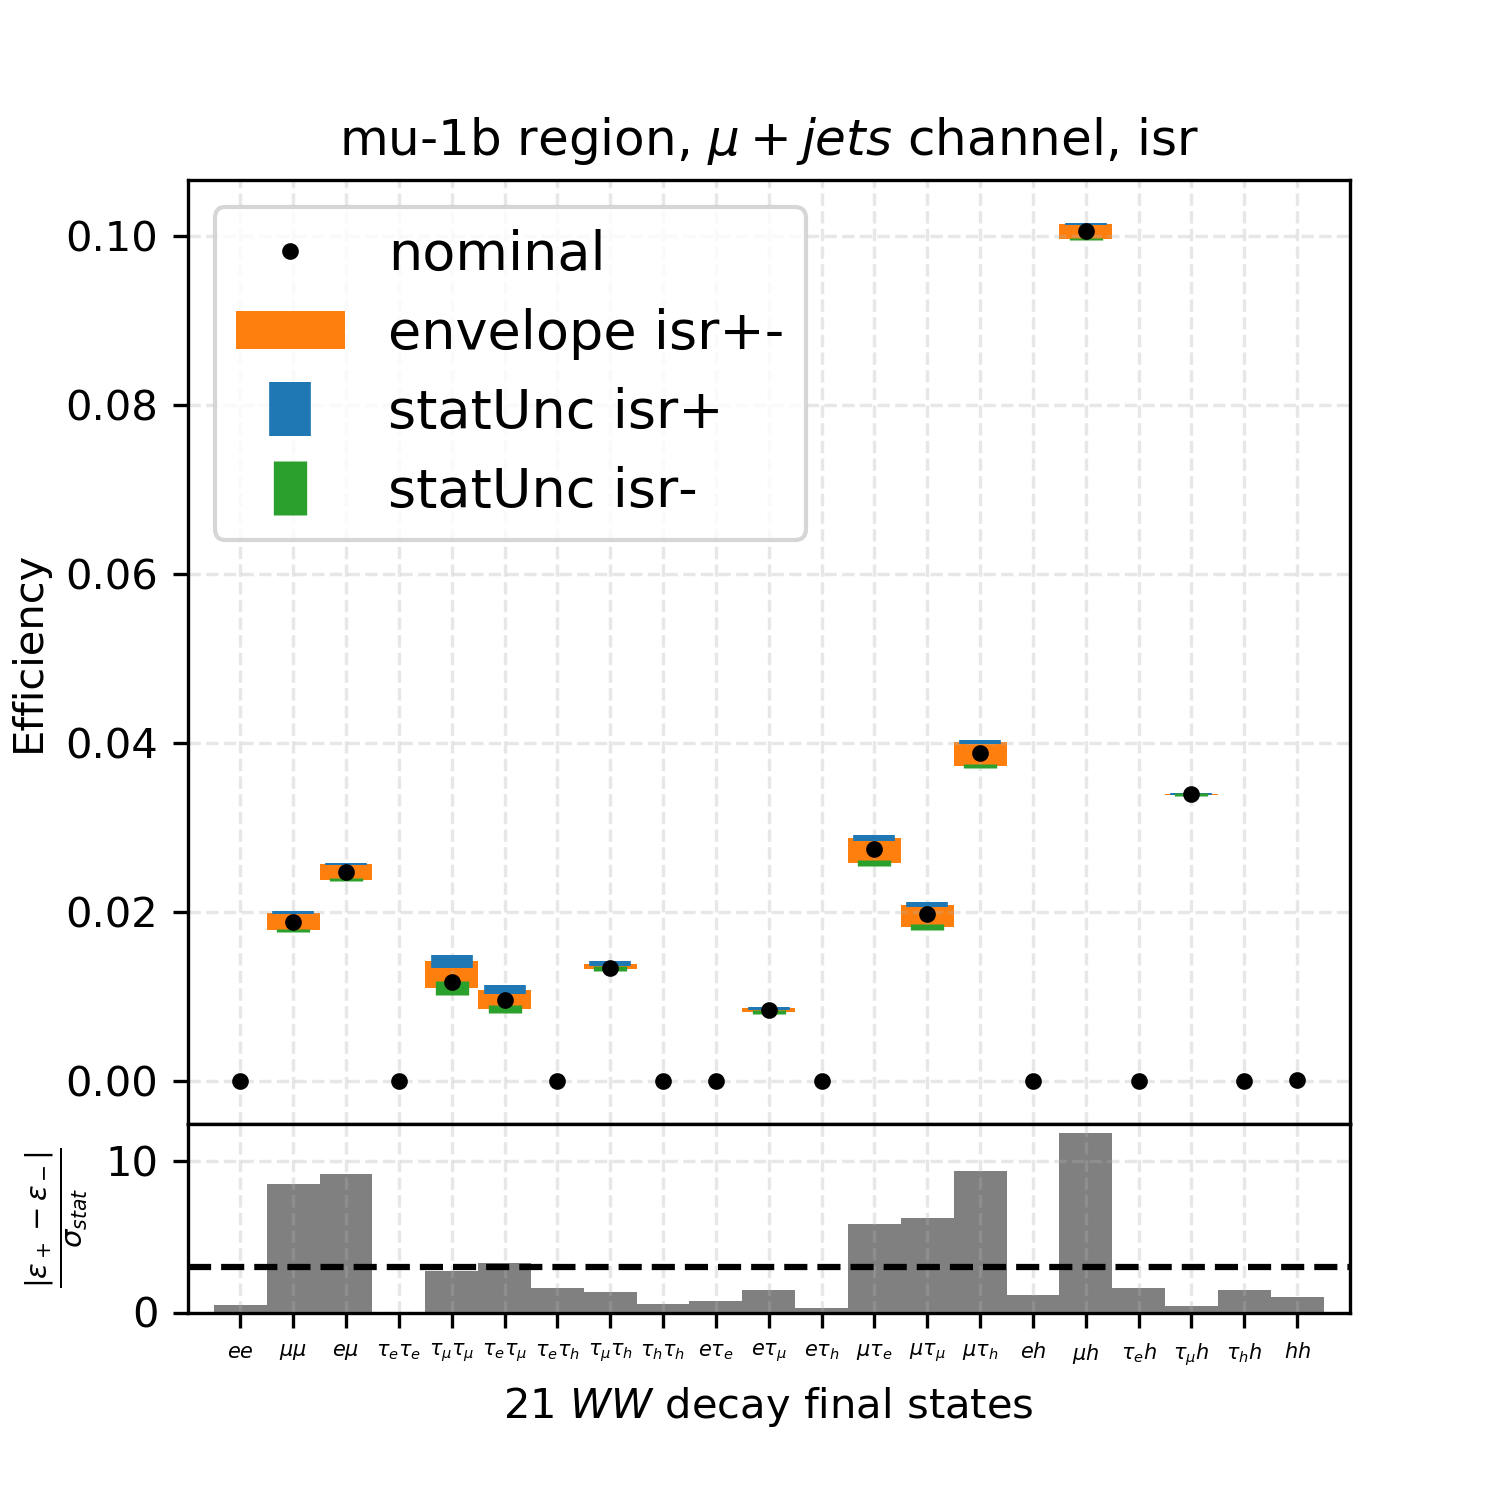
\includegraphics[width=0.24\textwidth]{chapters/Appendix/sectionTTSyst/figures/afterCorr/icata0_ch3_isr.png}

    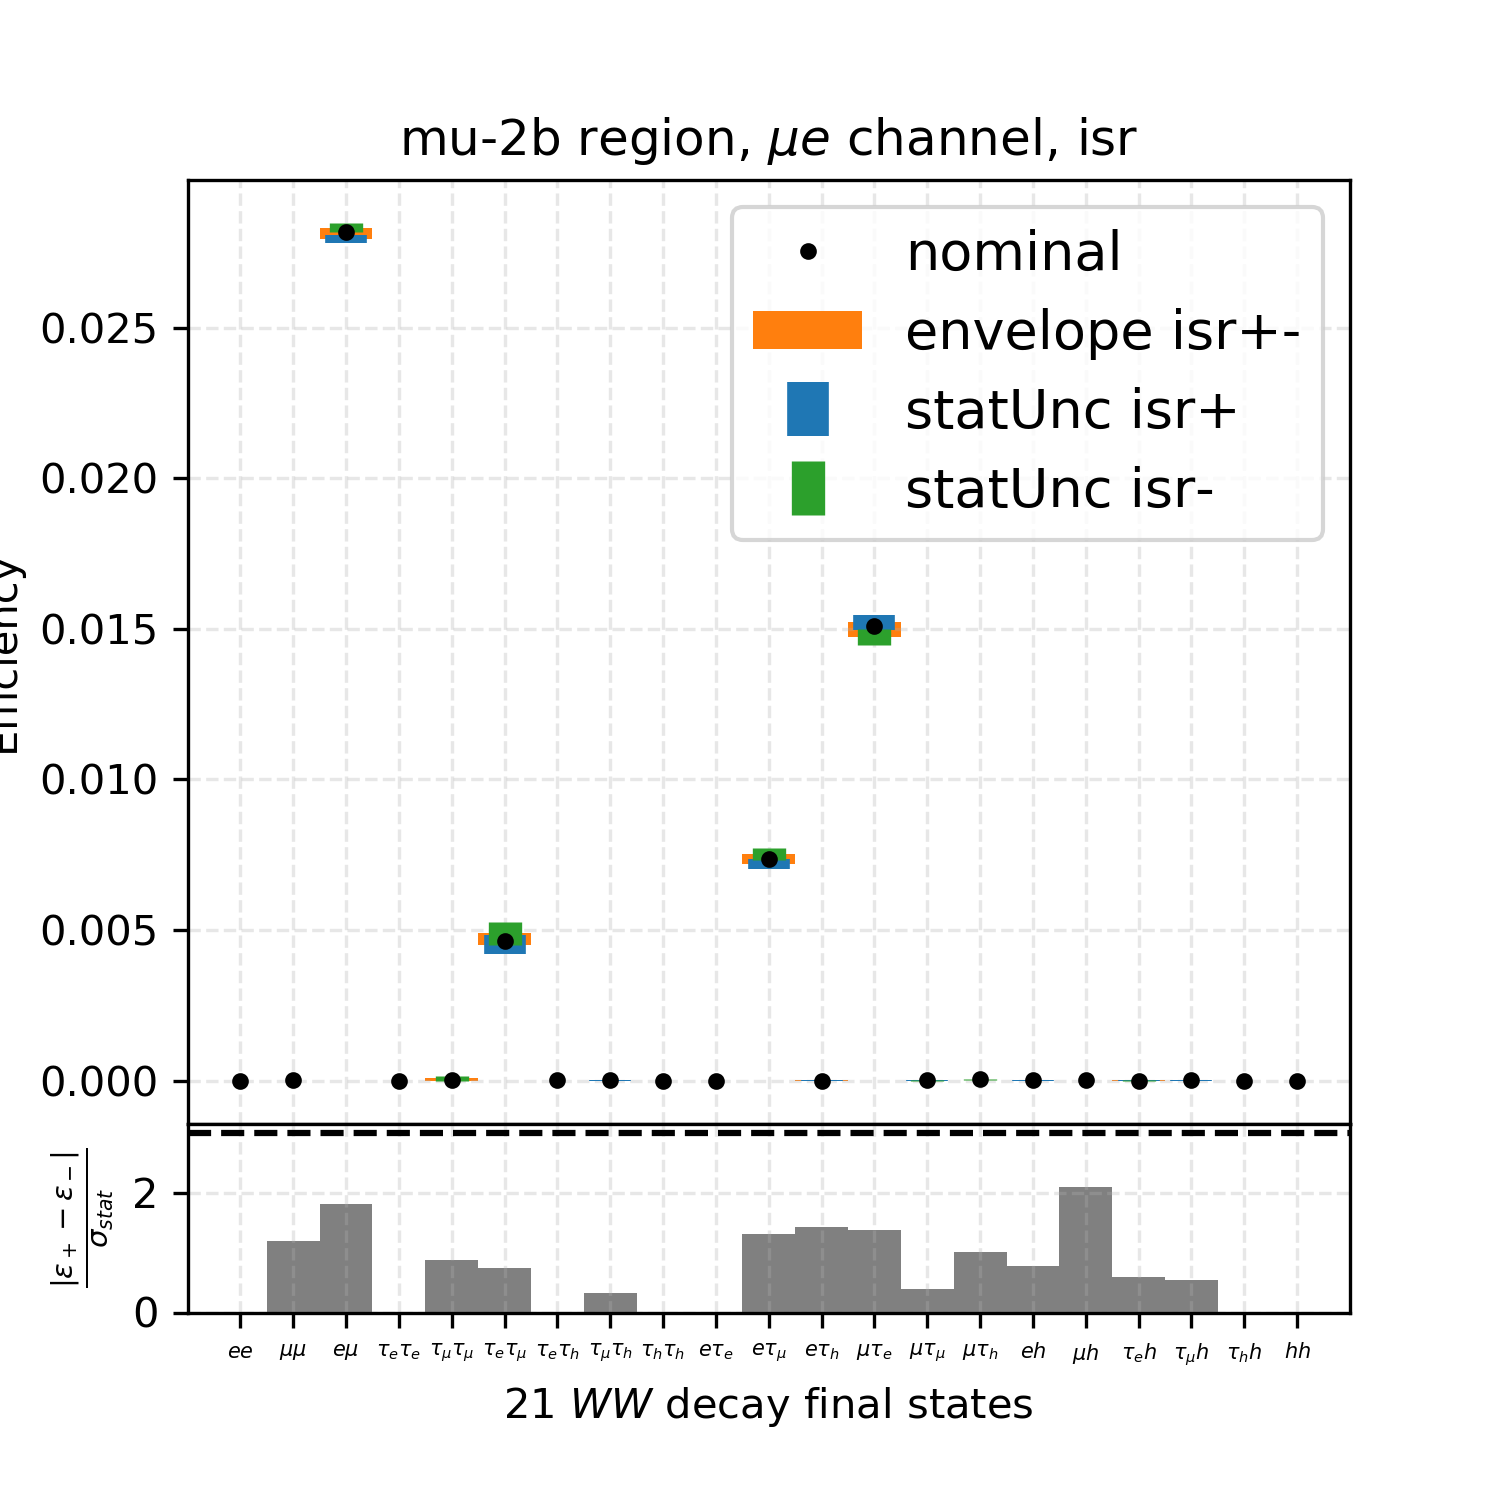
\includegraphics[width=0.24\textwidth]{chapters/Appendix/sectionTTSyst/figures/afterCorr/icata1_ch0_isr.png}
    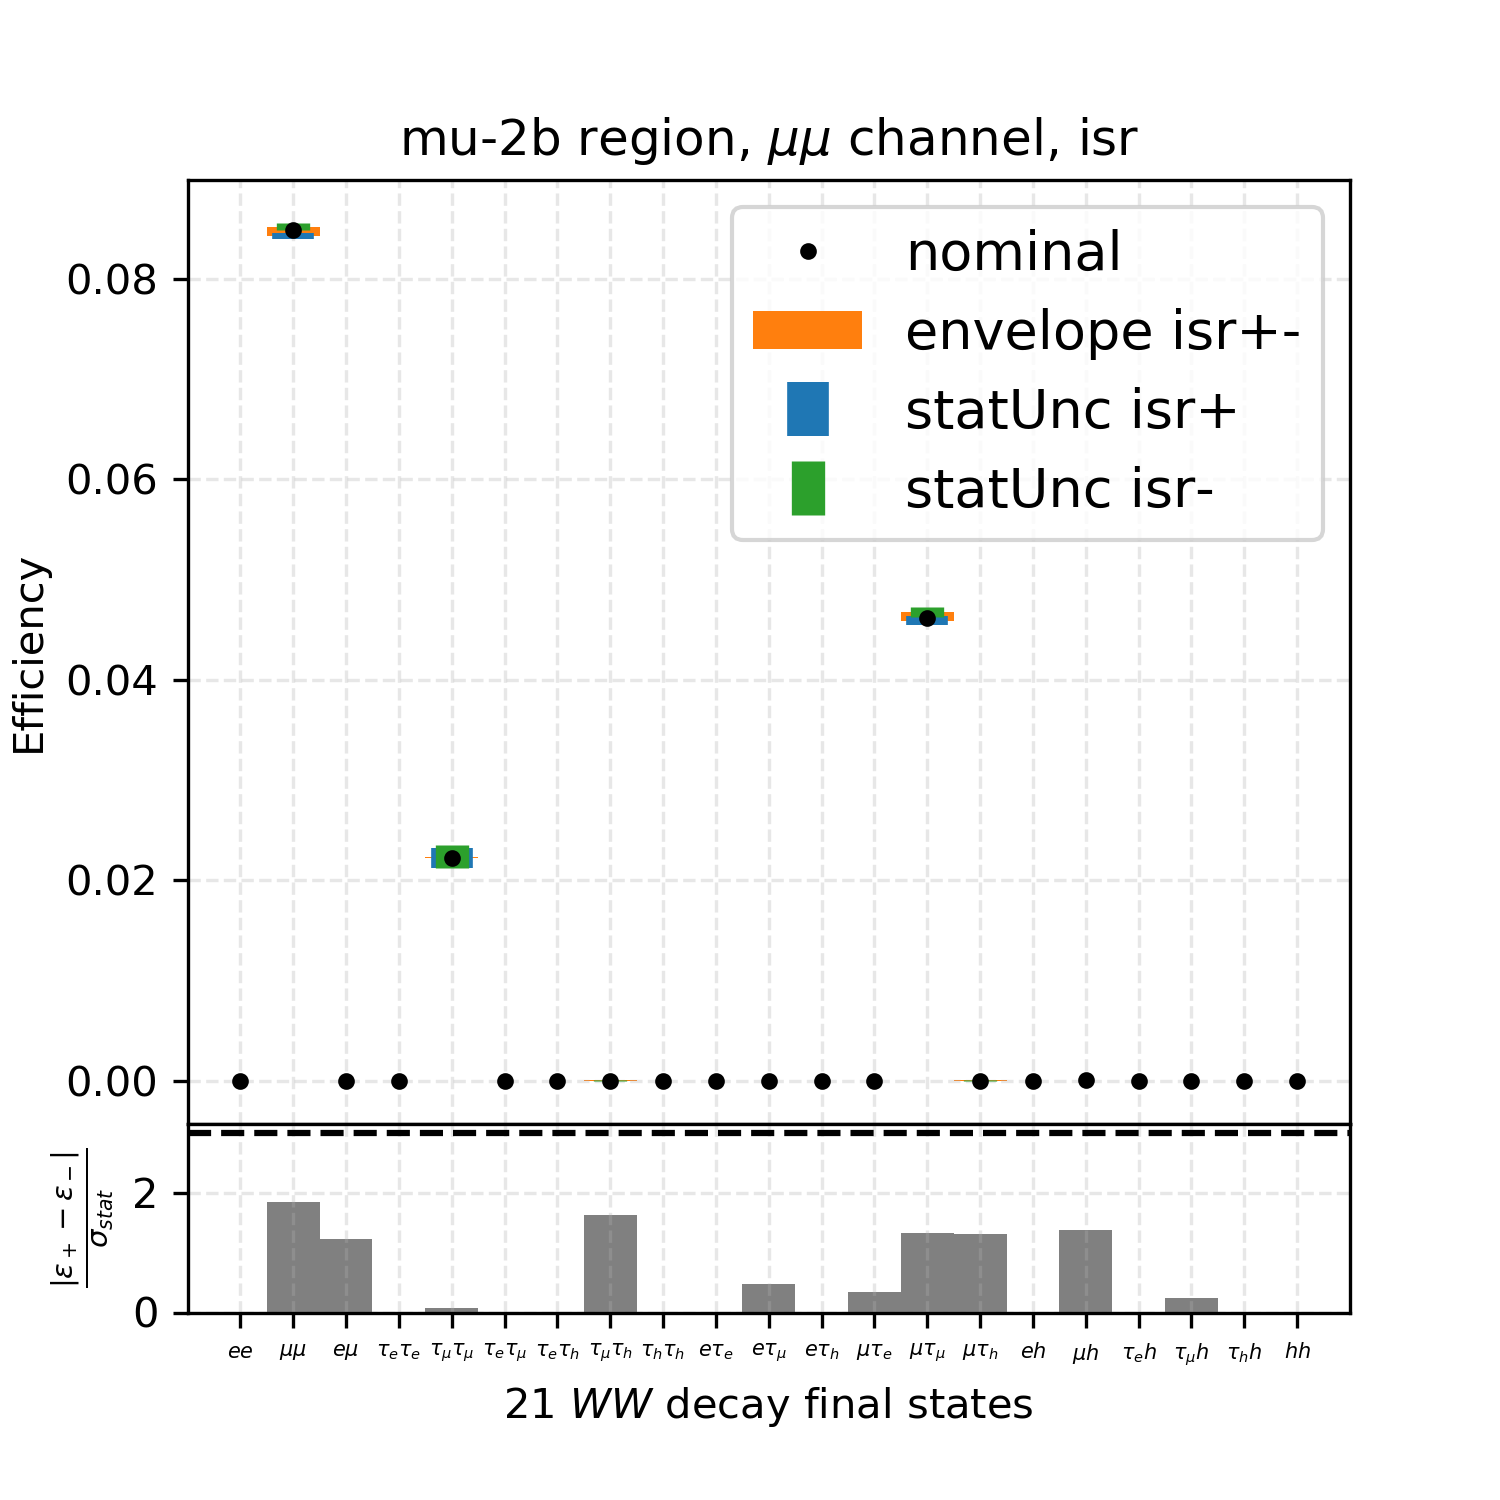
\includegraphics[width=0.24\textwidth]{chapters/Appendix/sectionTTSyst/figures/afterCorr/icata1_ch1_isr.png}
    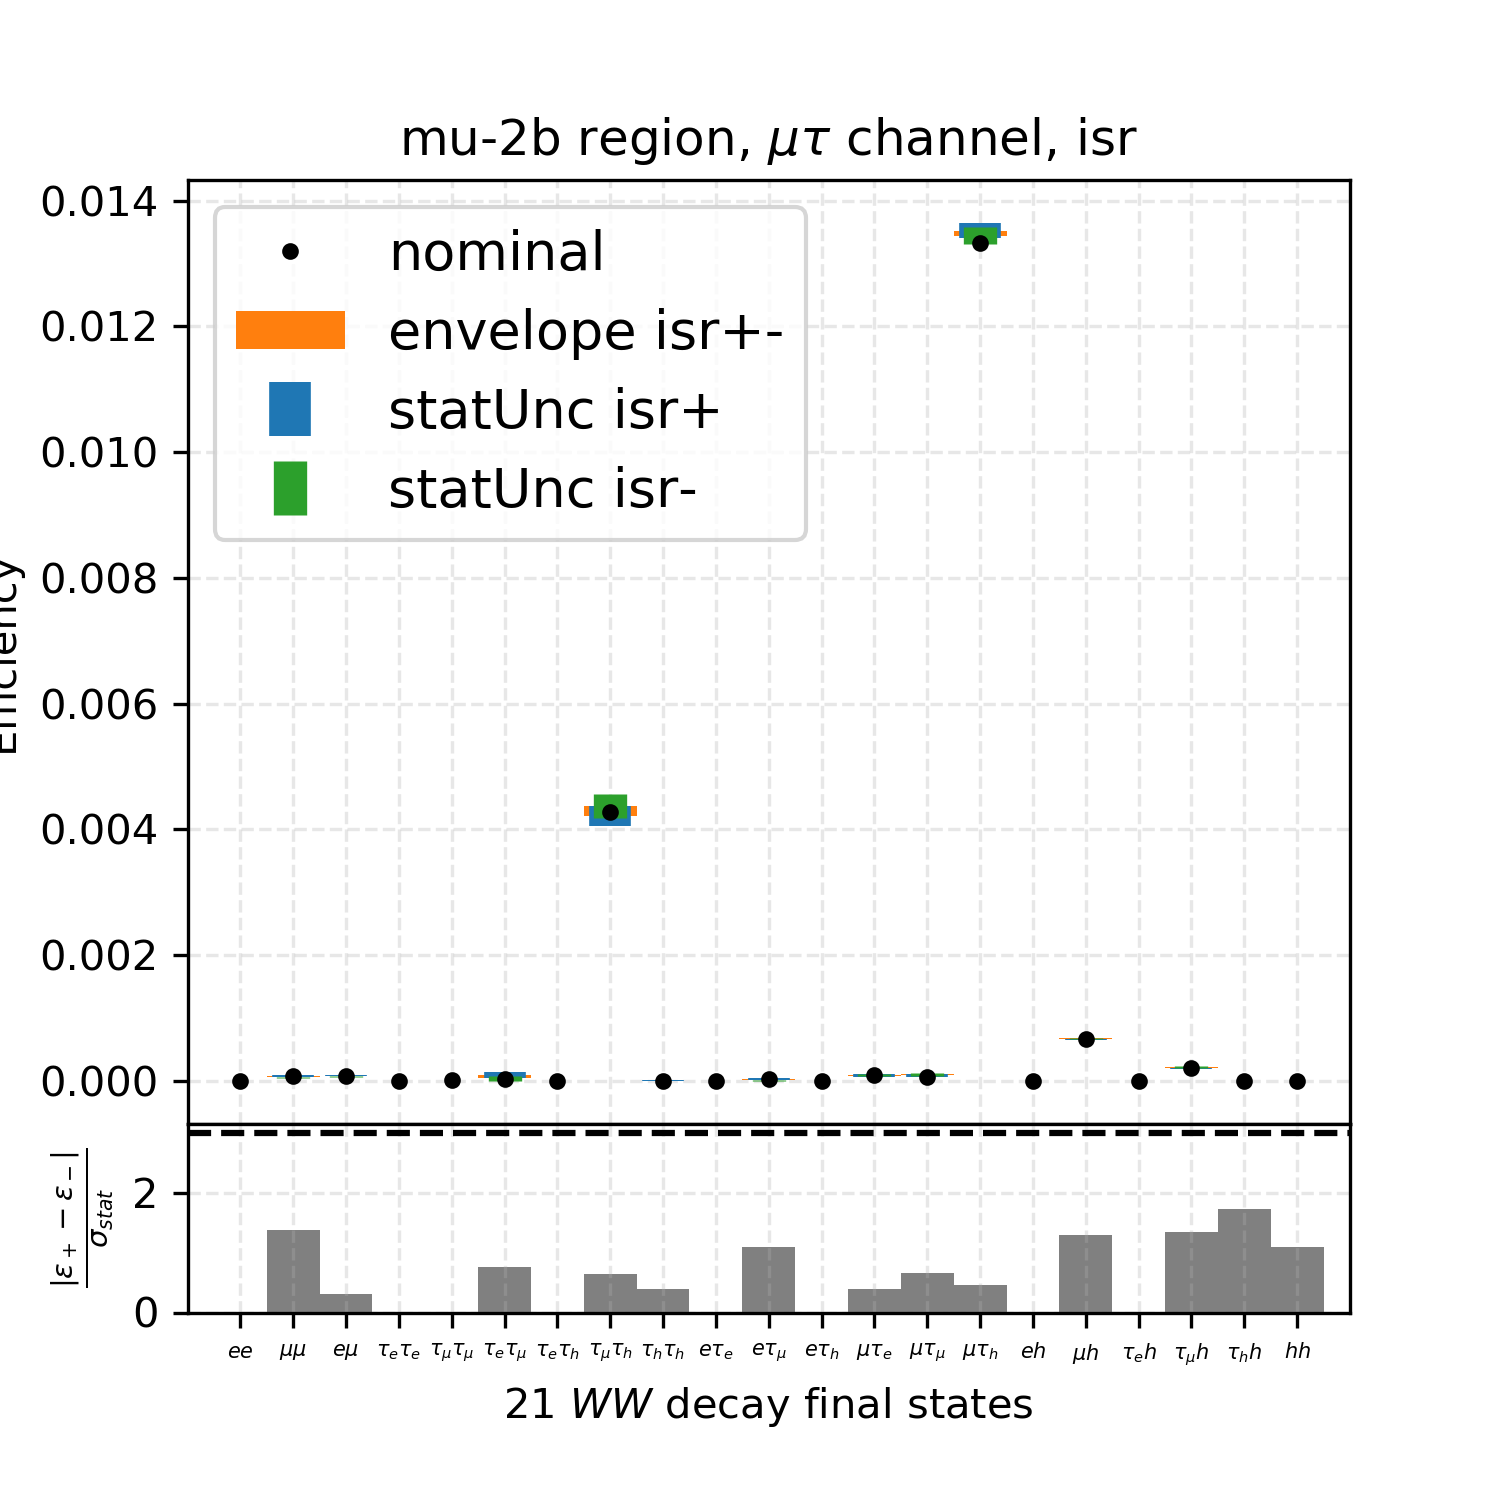
\includegraphics[width=0.24\textwidth]{chapters/Appendix/sectionTTSyst/figures/afterCorr/icata1_ch2_isr.png}
    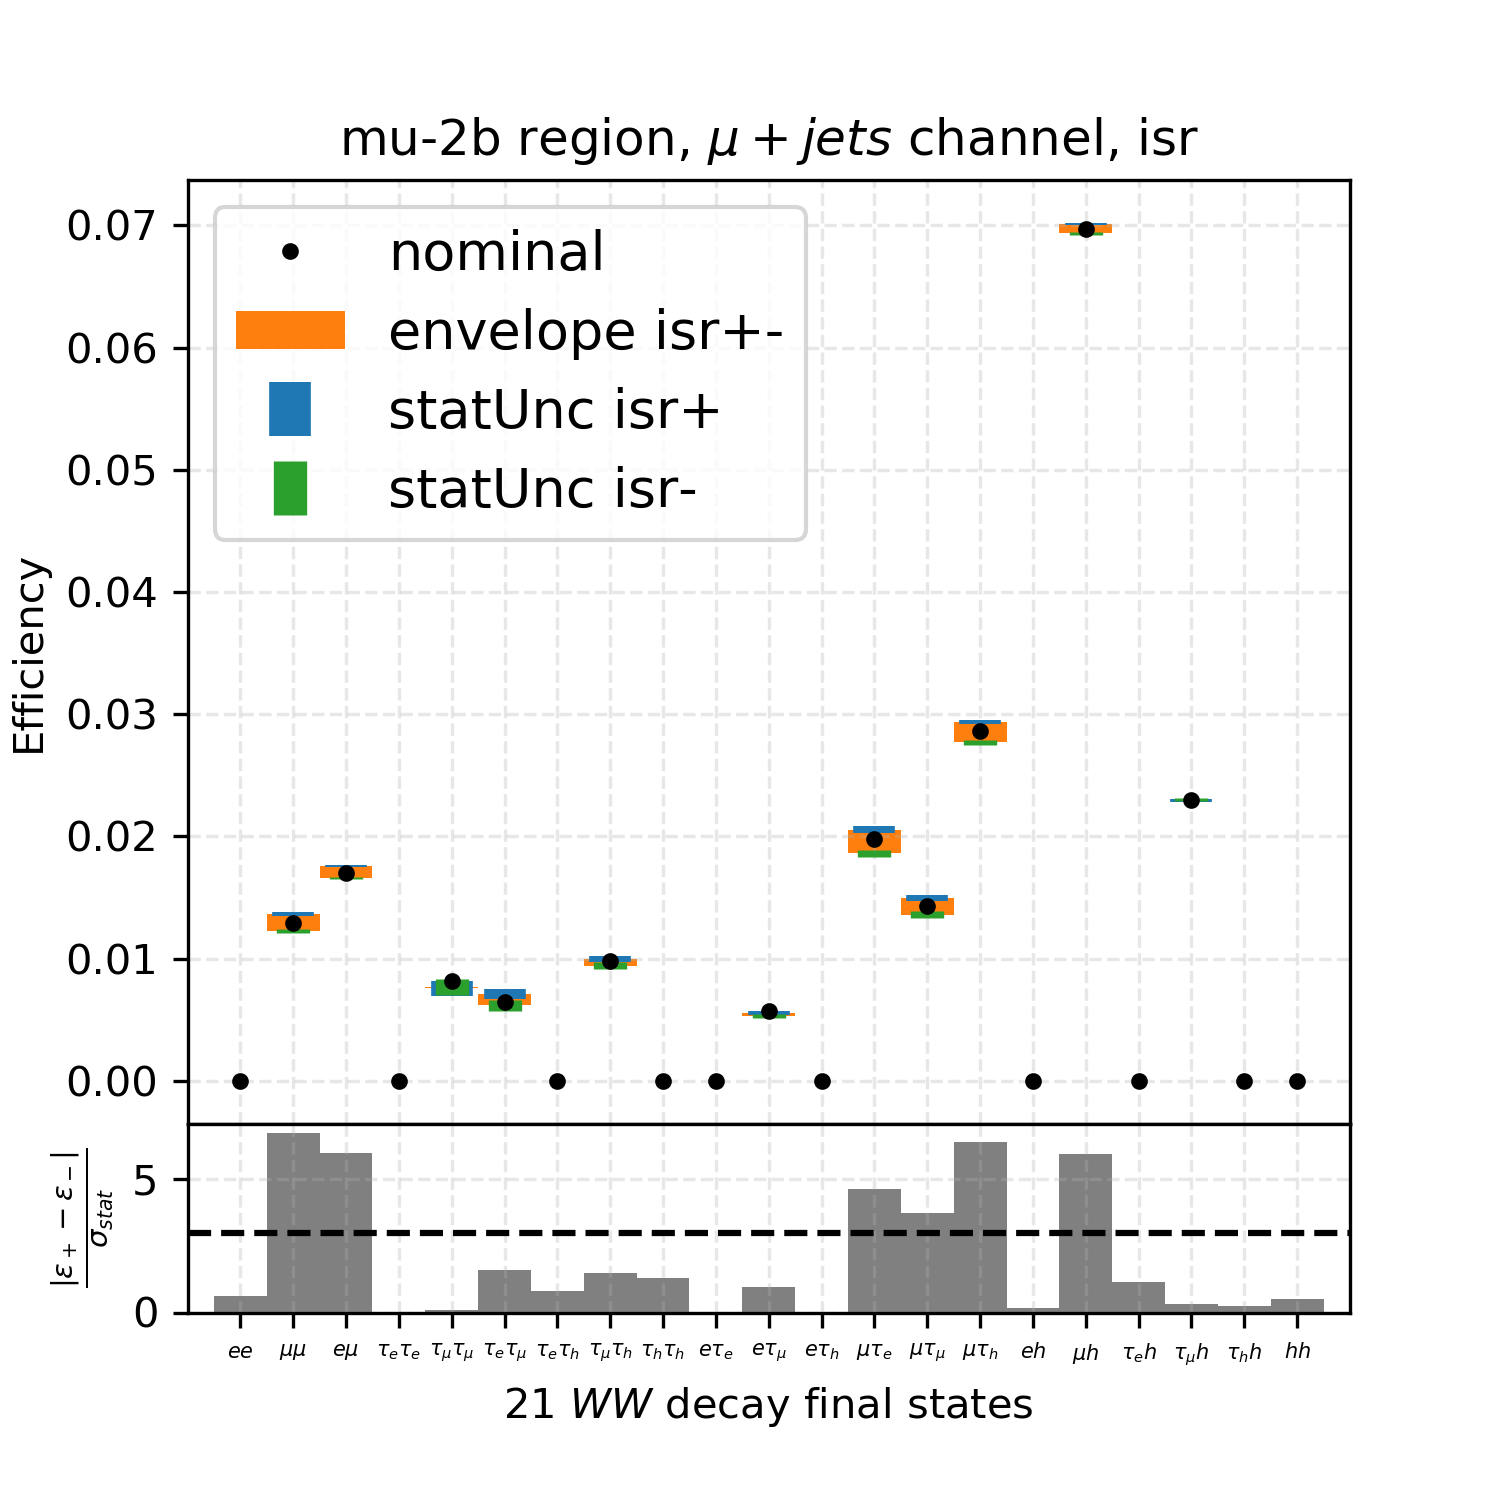
\includegraphics[width=0.24\textwidth]{chapters/Appendix/sectionTTSyst/figures/afterCorr/icata1_ch3_isr.png}
    
    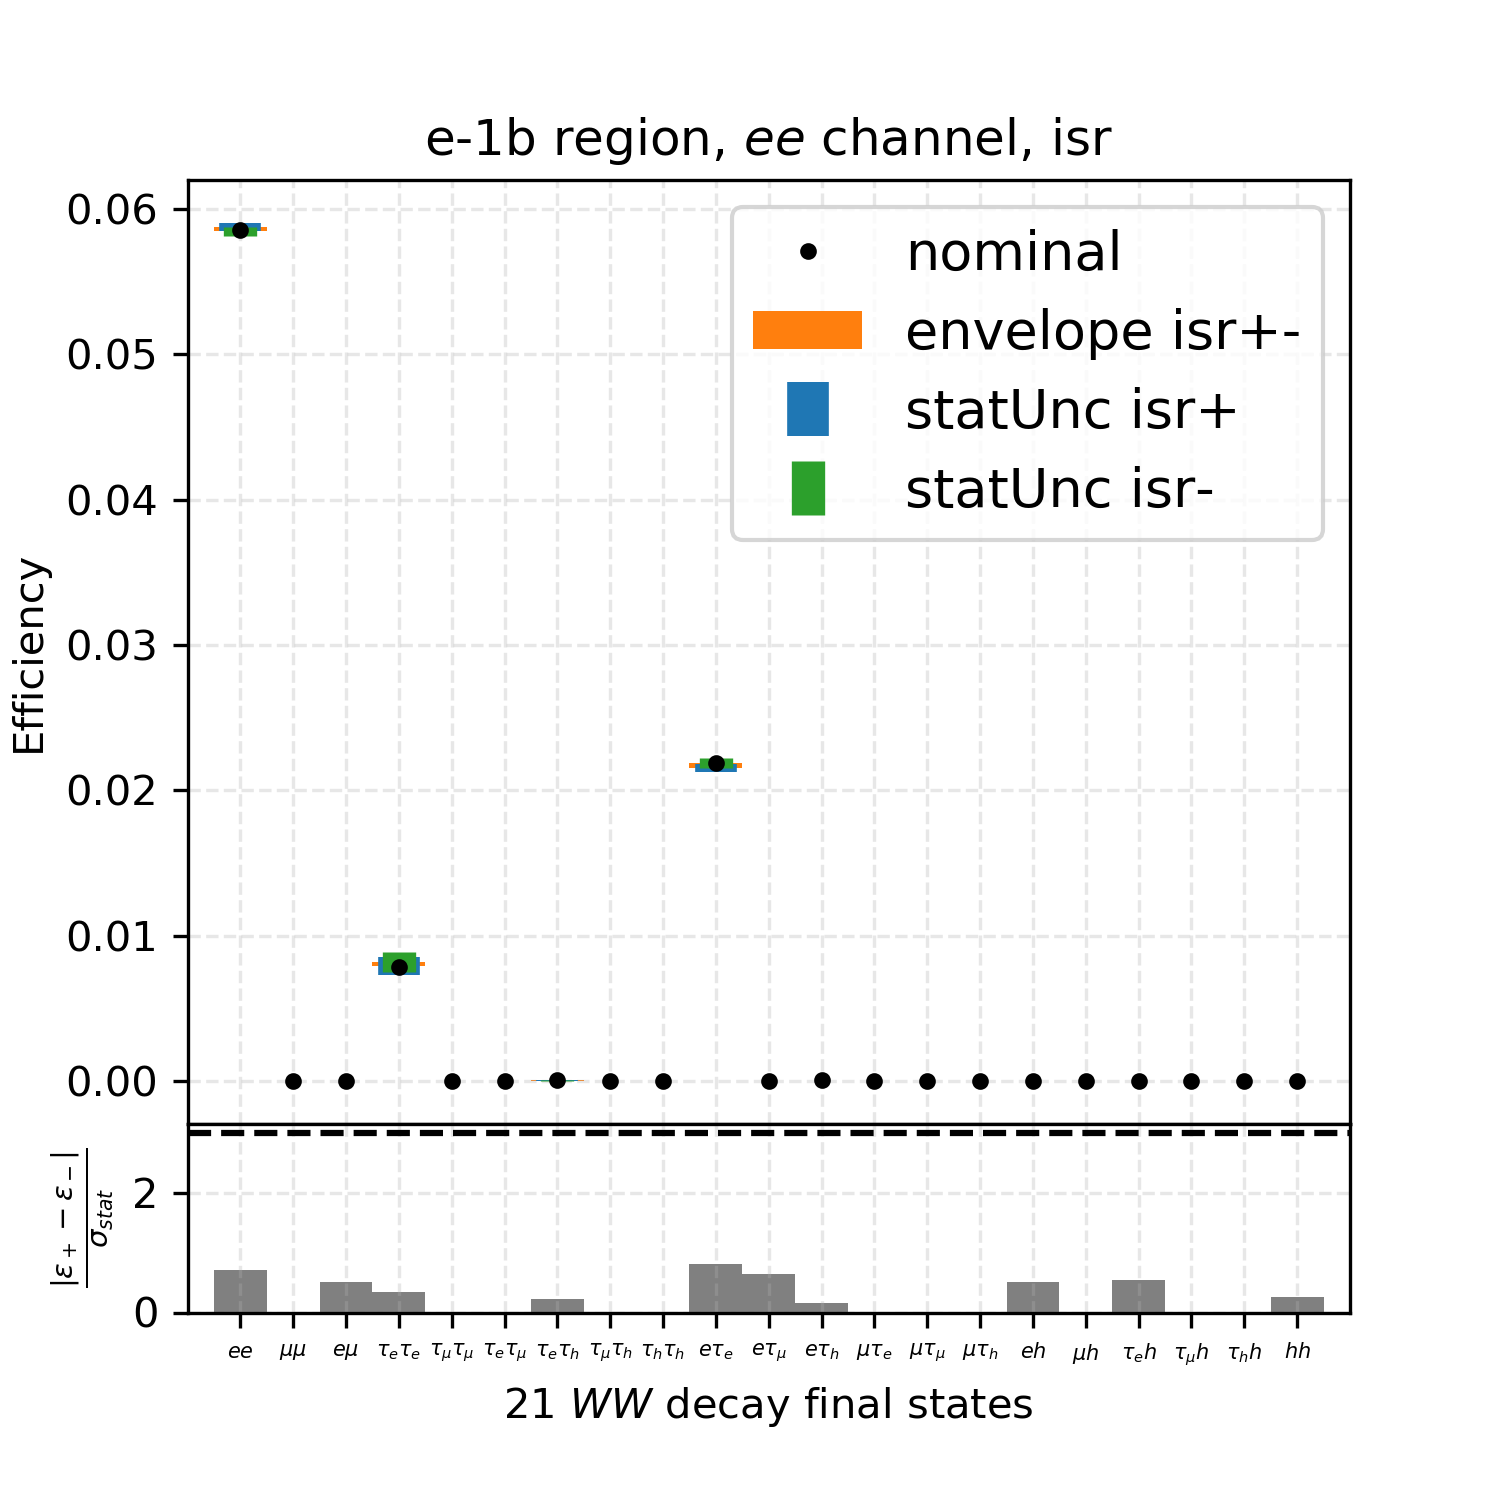
\includegraphics[width=0.24\textwidth]{chapters/Appendix/sectionTTSyst/figures/afterCorr/icata2_ch0_isr.png}
    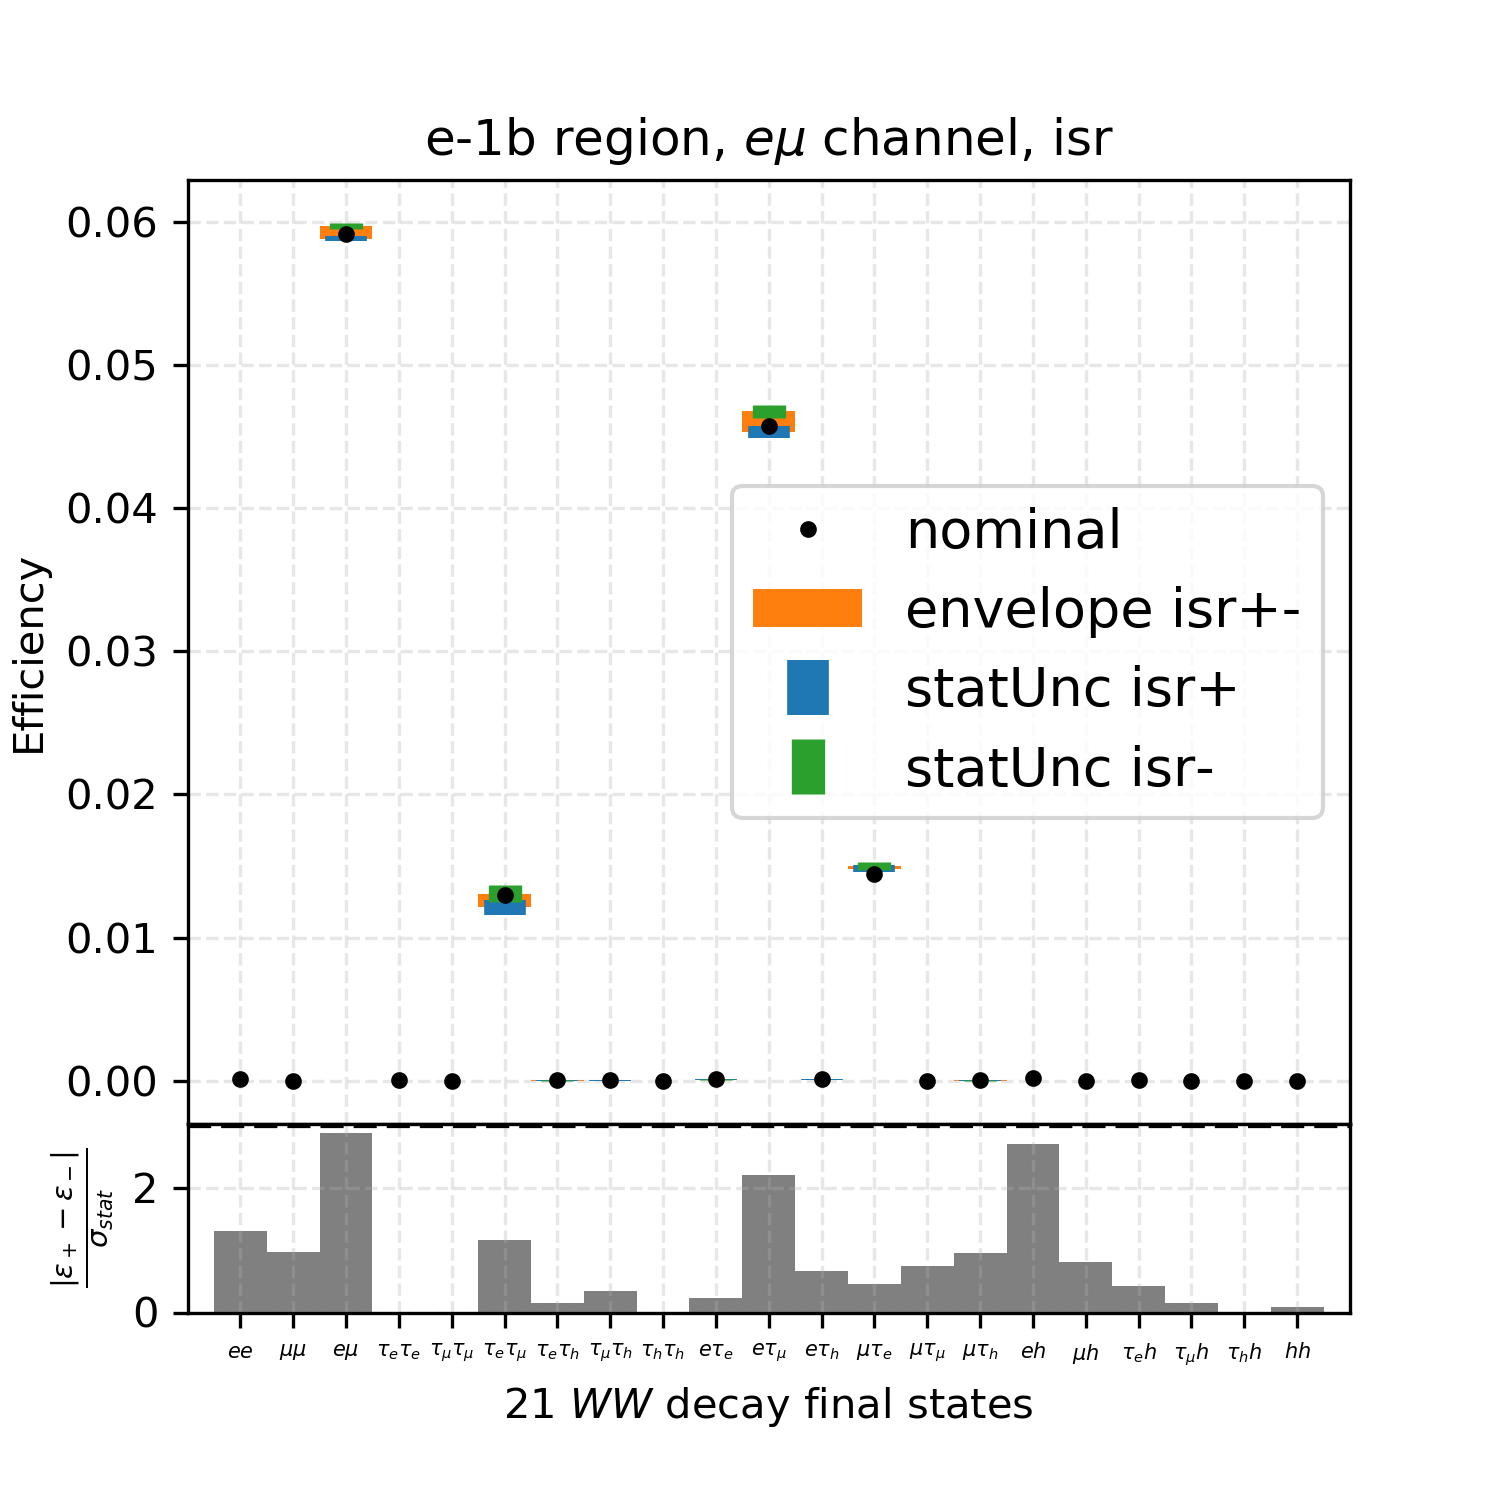
\includegraphics[width=0.24\textwidth]{chapters/Appendix/sectionTTSyst/figures/afterCorr/icata2_ch1_isr.png}
    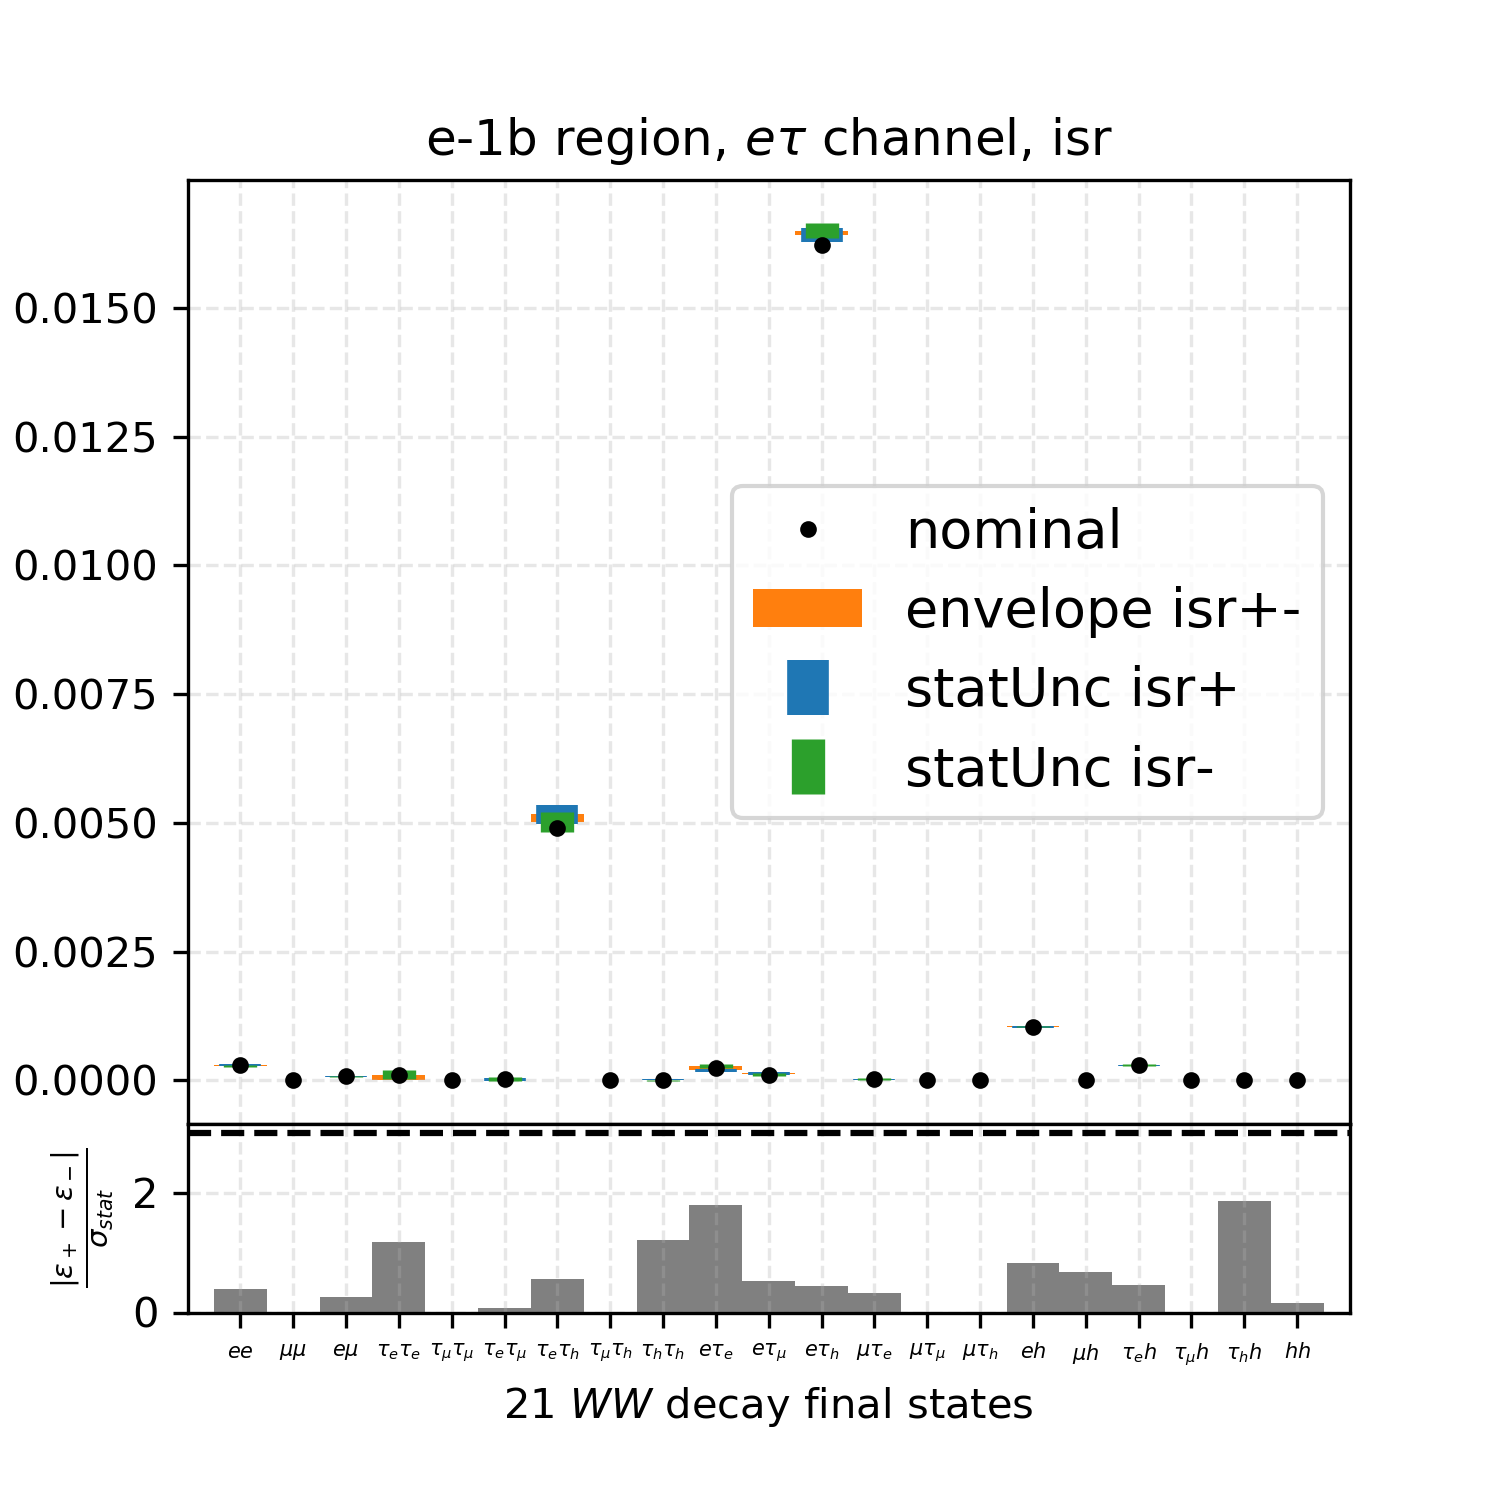
\includegraphics[width=0.24\textwidth]{chapters/Appendix/sectionTTSyst/figures/afterCorr/icata2_ch2_isr.png}
    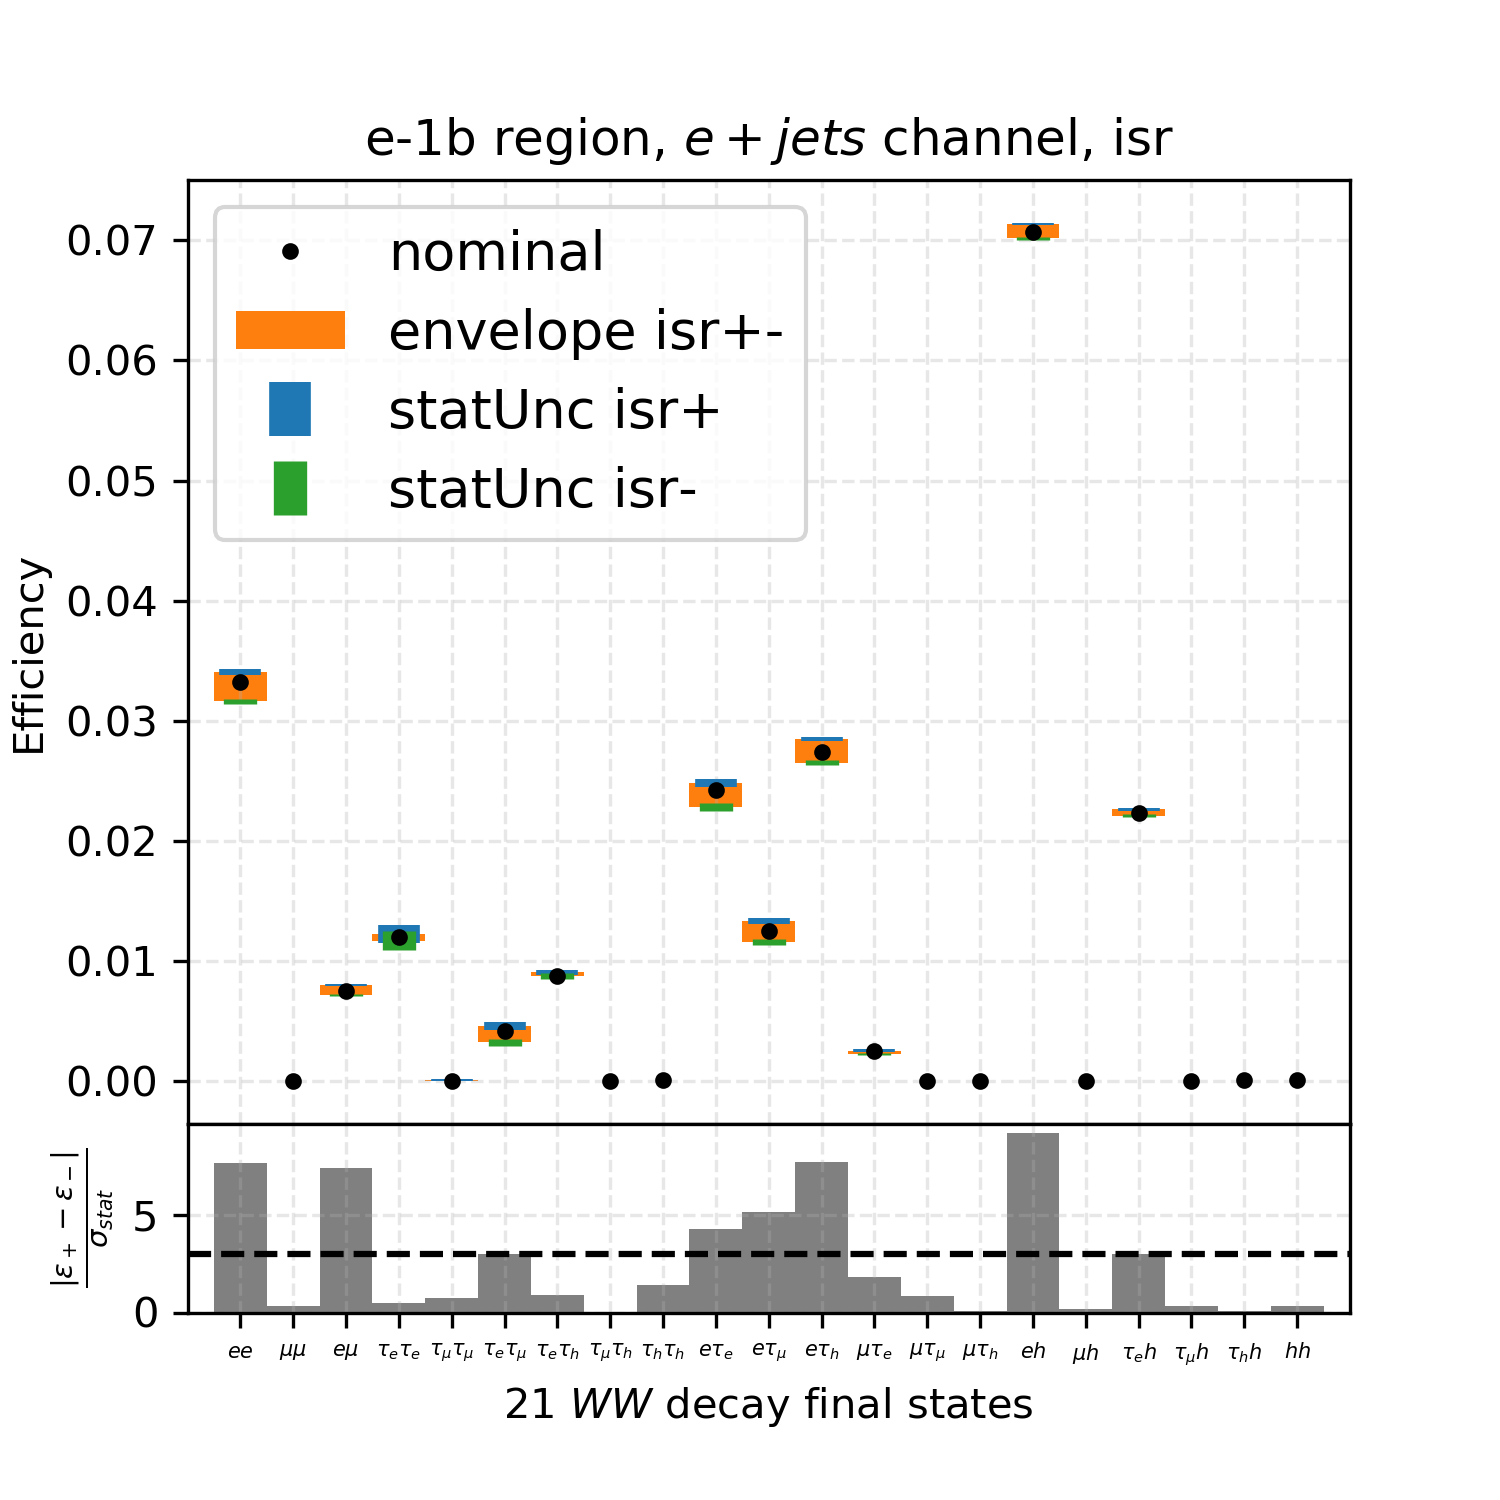
\includegraphics[width=0.24\textwidth]{chapters/Appendix/sectionTTSyst/figures/afterCorr/icata2_ch3_isr.png}

    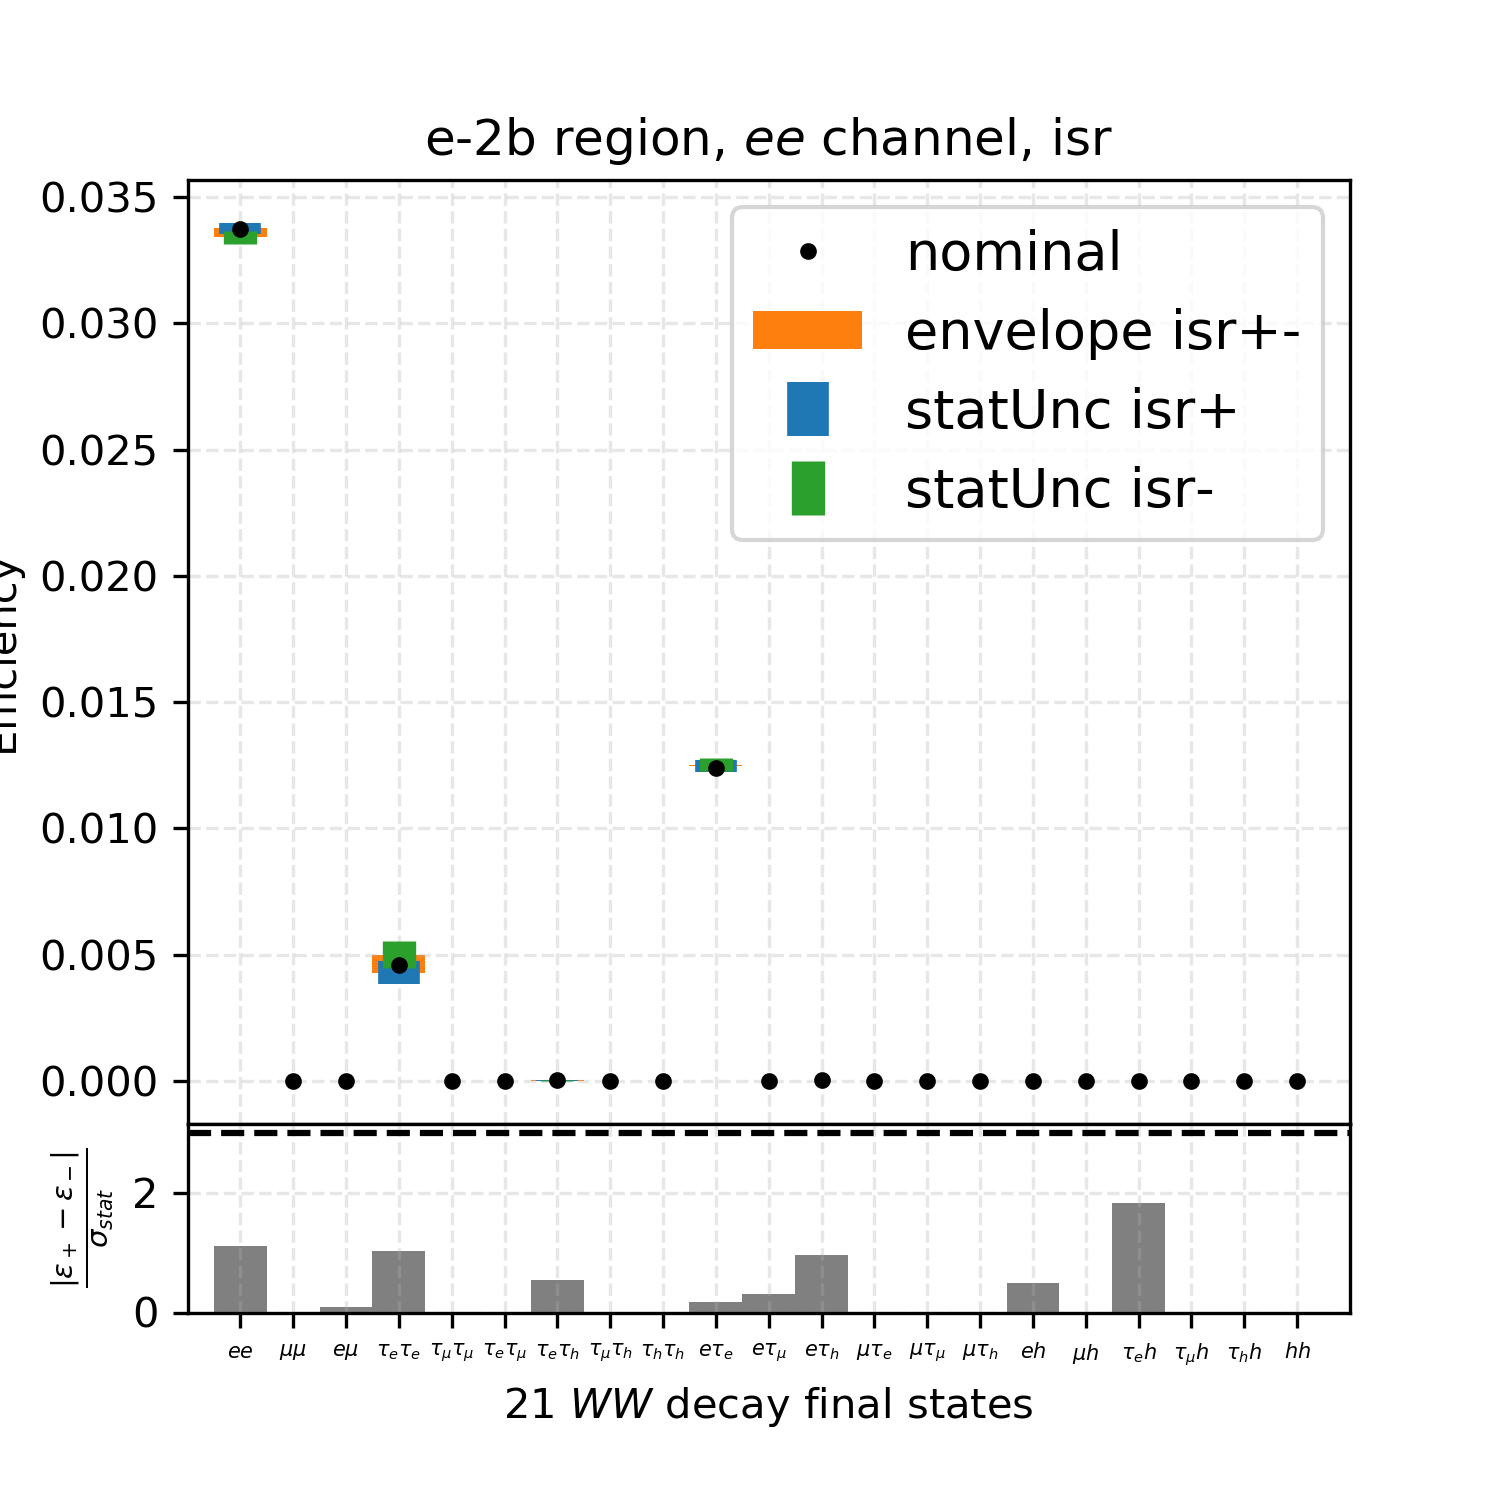
\includegraphics[width=0.24\textwidth]{chapters/Appendix/sectionTTSyst/figures/afterCorr/icata3_ch0_isr.png}
    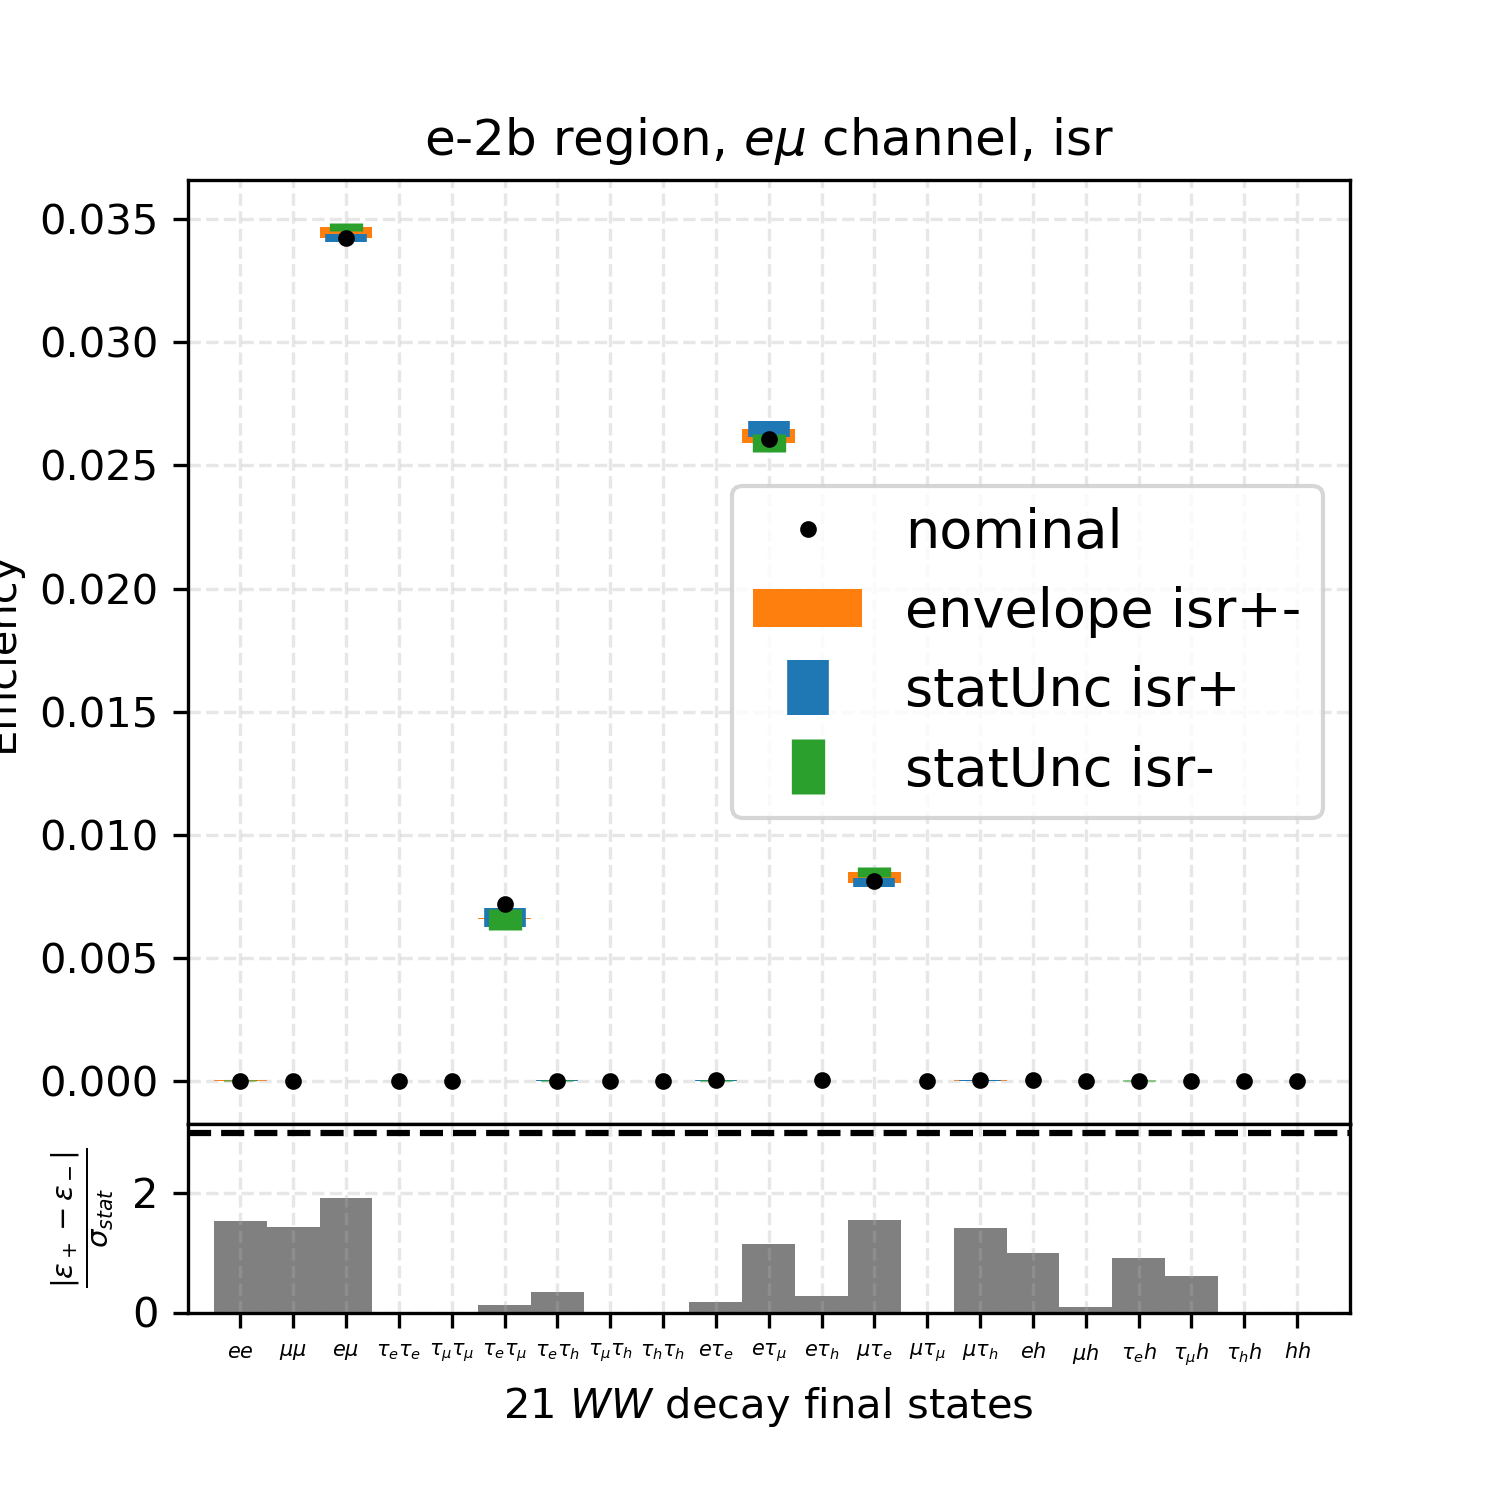
\includegraphics[width=0.24\textwidth]{chapters/Appendix/sectionTTSyst/figures/afterCorr/icata3_ch1_isr.png}
    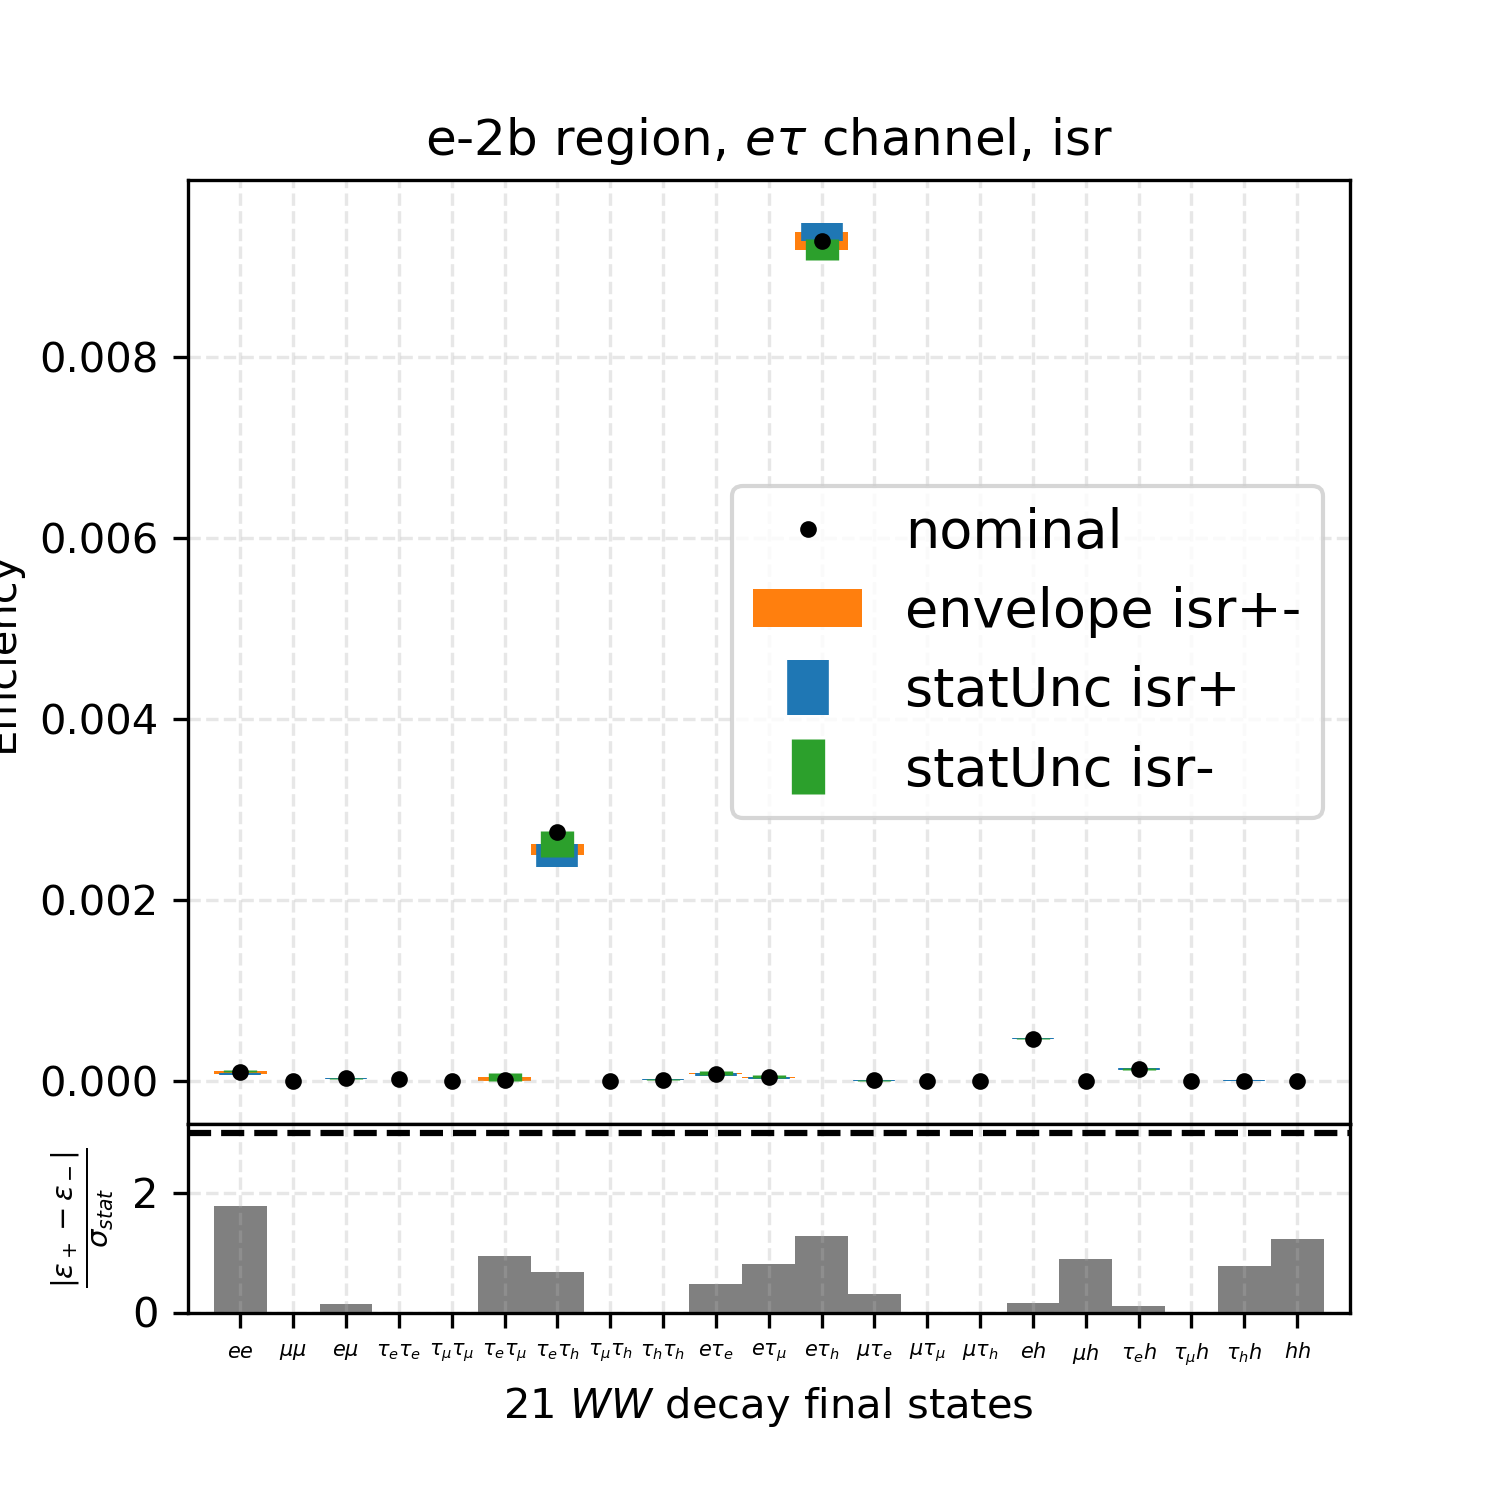
\includegraphics[width=0.24\textwidth]{chapters/Appendix/sectionTTSyst/figures/afterCorr/icata3_ch2_isr.png}
    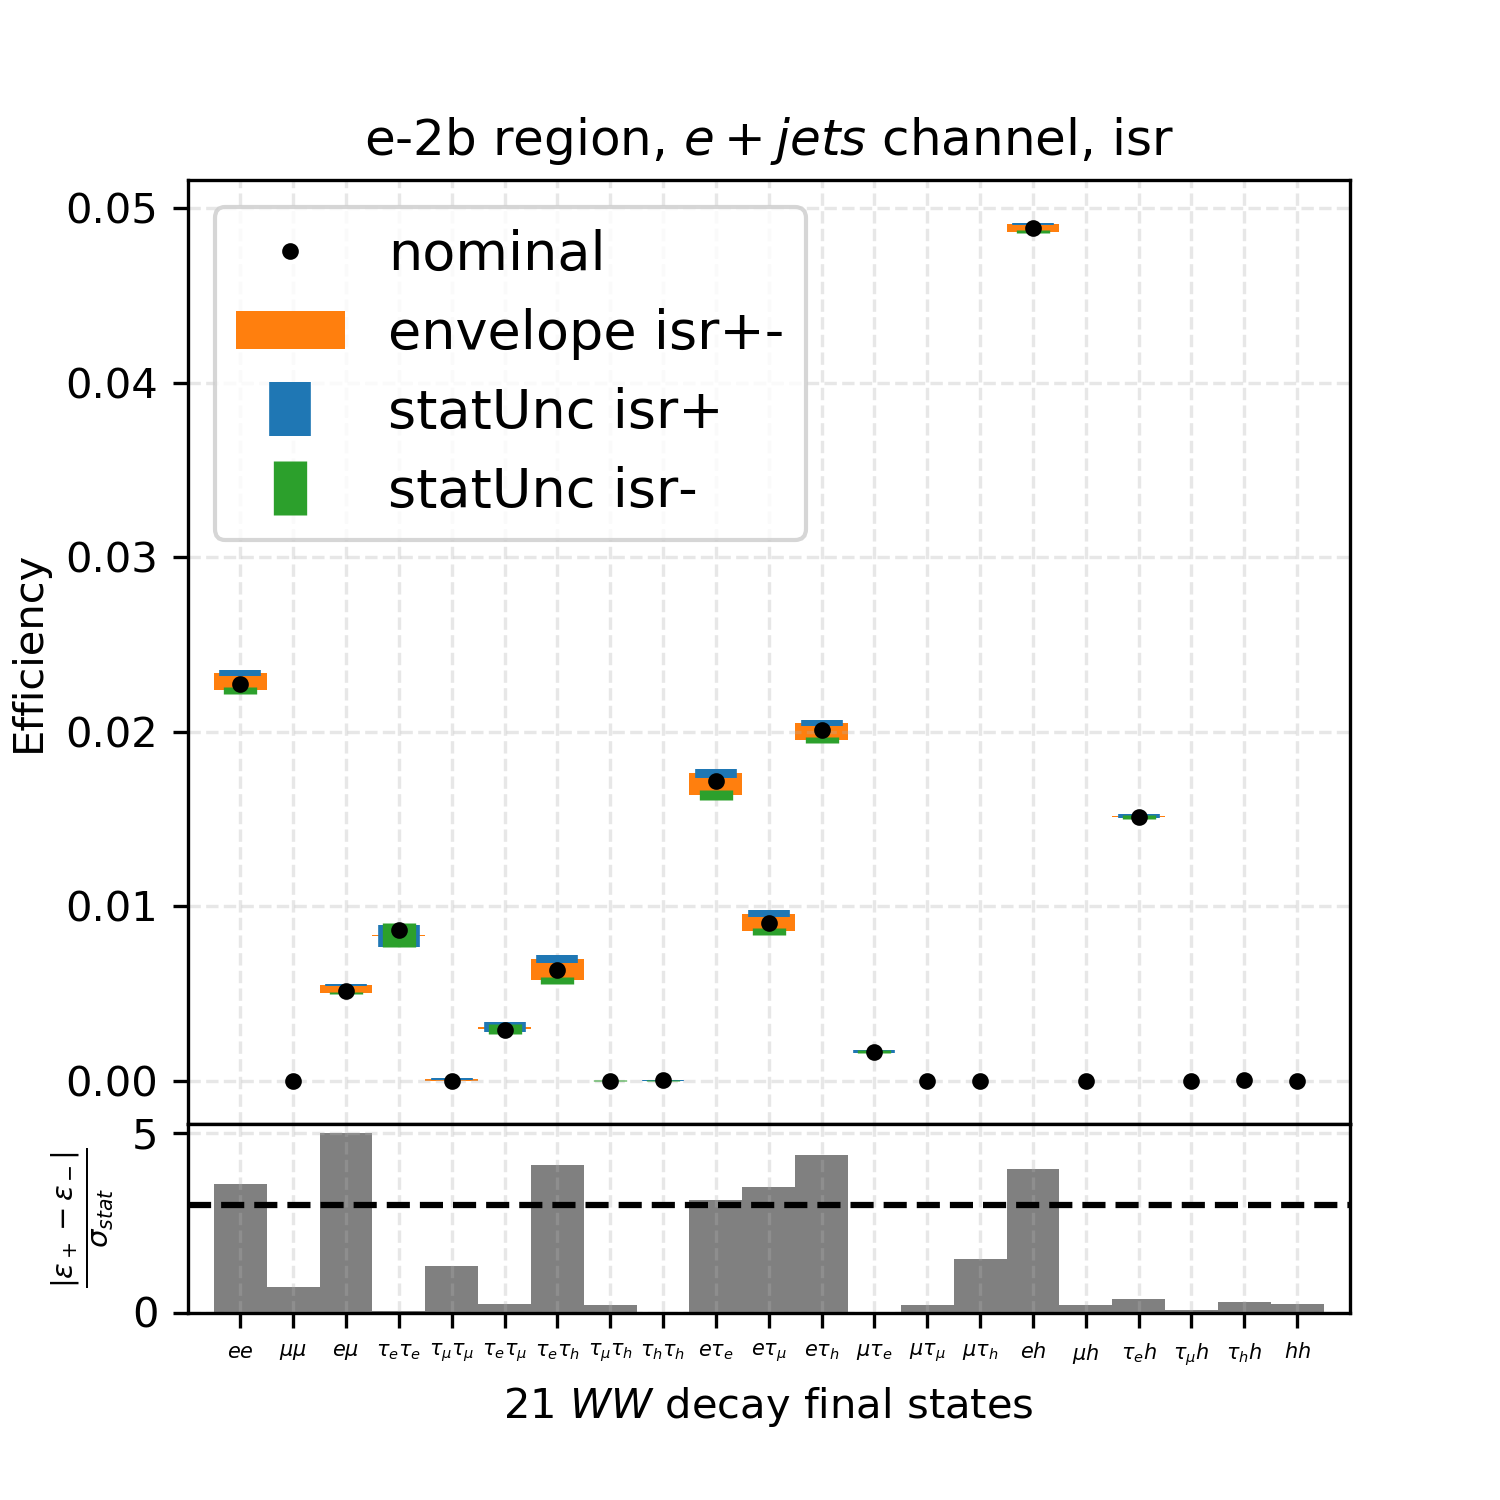
\includegraphics[width=0.24\textwidth]{chapters/Appendix/sectionTTSyst/figures/afterCorr/icata3_ch3_isr.png}
    
    \caption{Reweight $\tau_h$ and $j \to \tau_h$ efficiencies in the dedicated FSR, ISF, MEPS, UE ttbar samples}
    \label{fig:appendix:reweighttt:effAfterCorrFSR}
\end{figure}




\begin{figure}
    \centering
    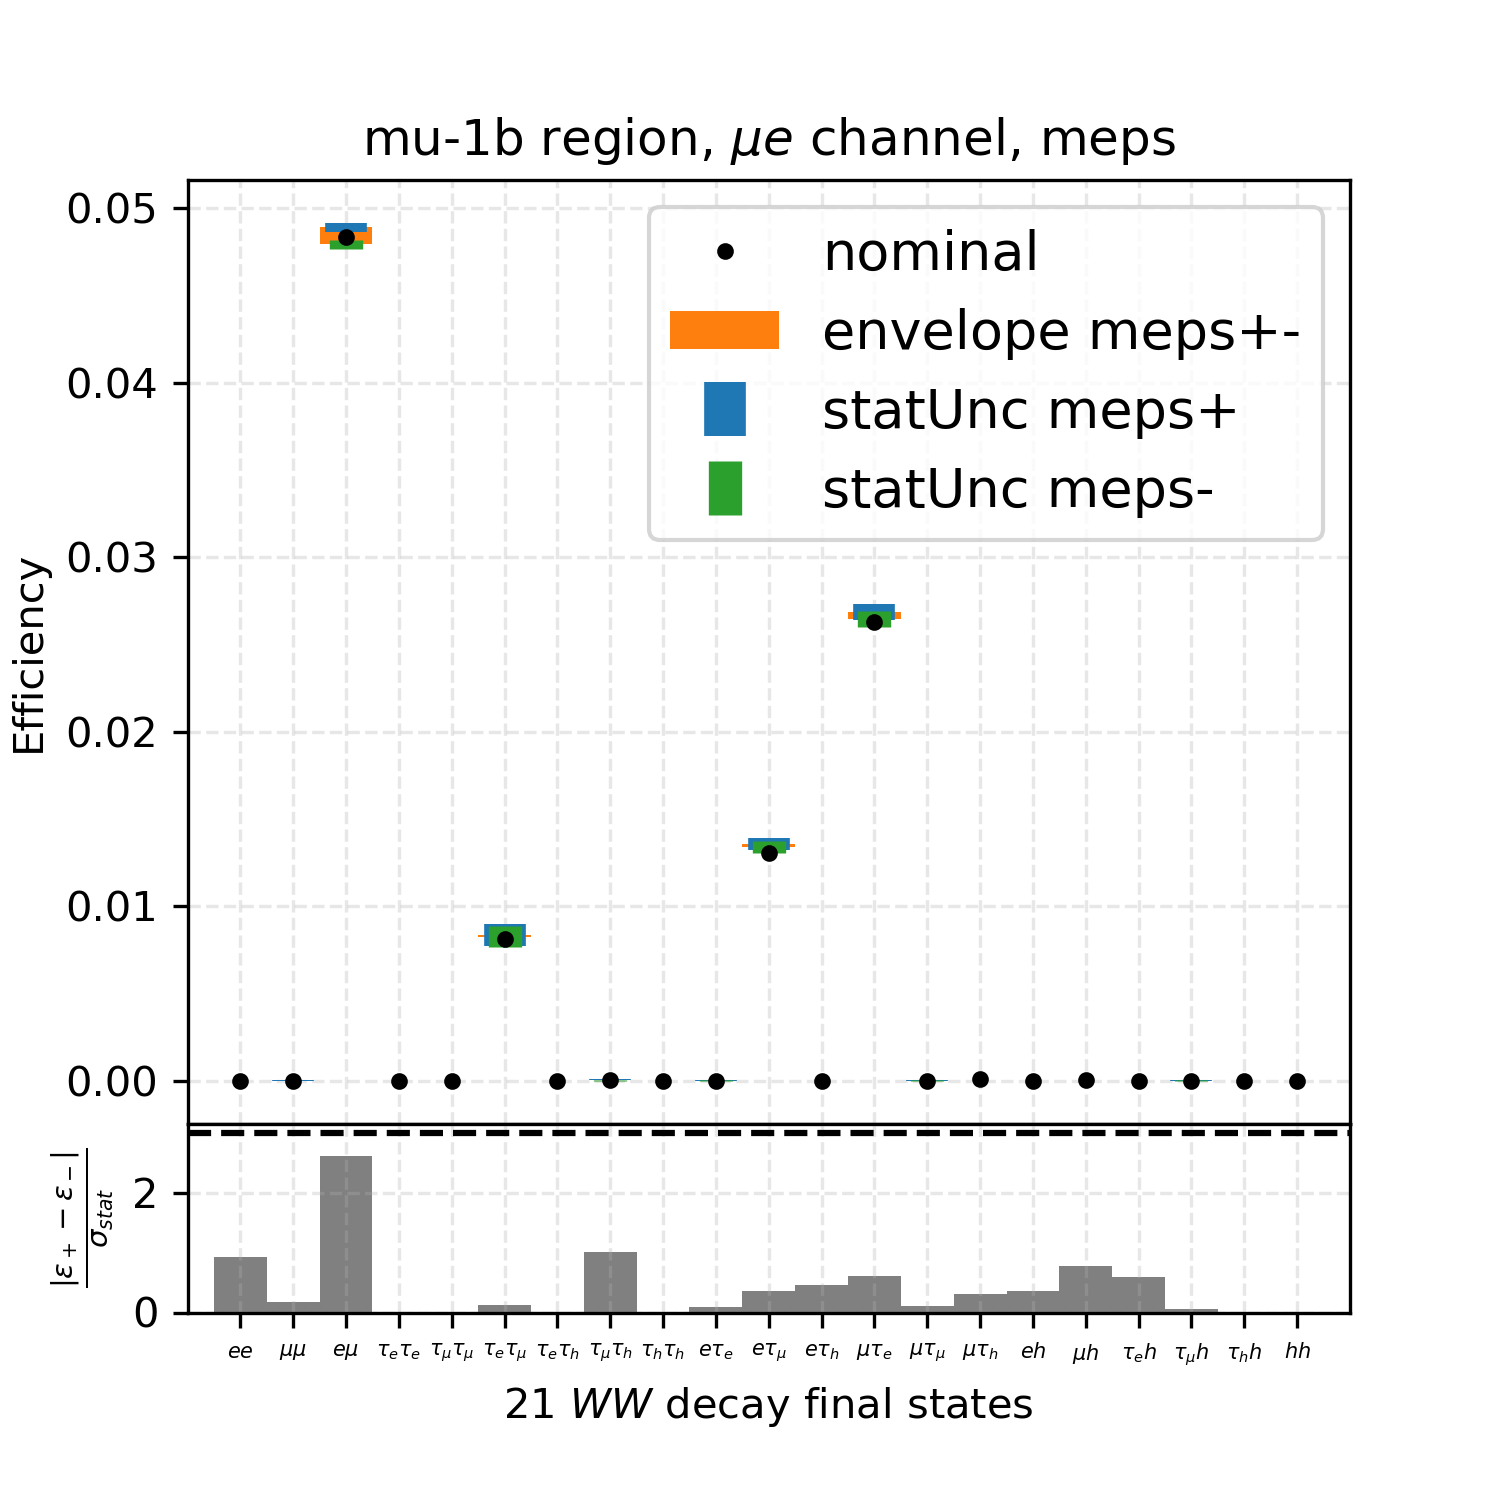
\includegraphics[width=0.24\textwidth]{chapters/Appendix/sectionTTSyst/figures/afterCorr/icata0_ch0_meps.png}
    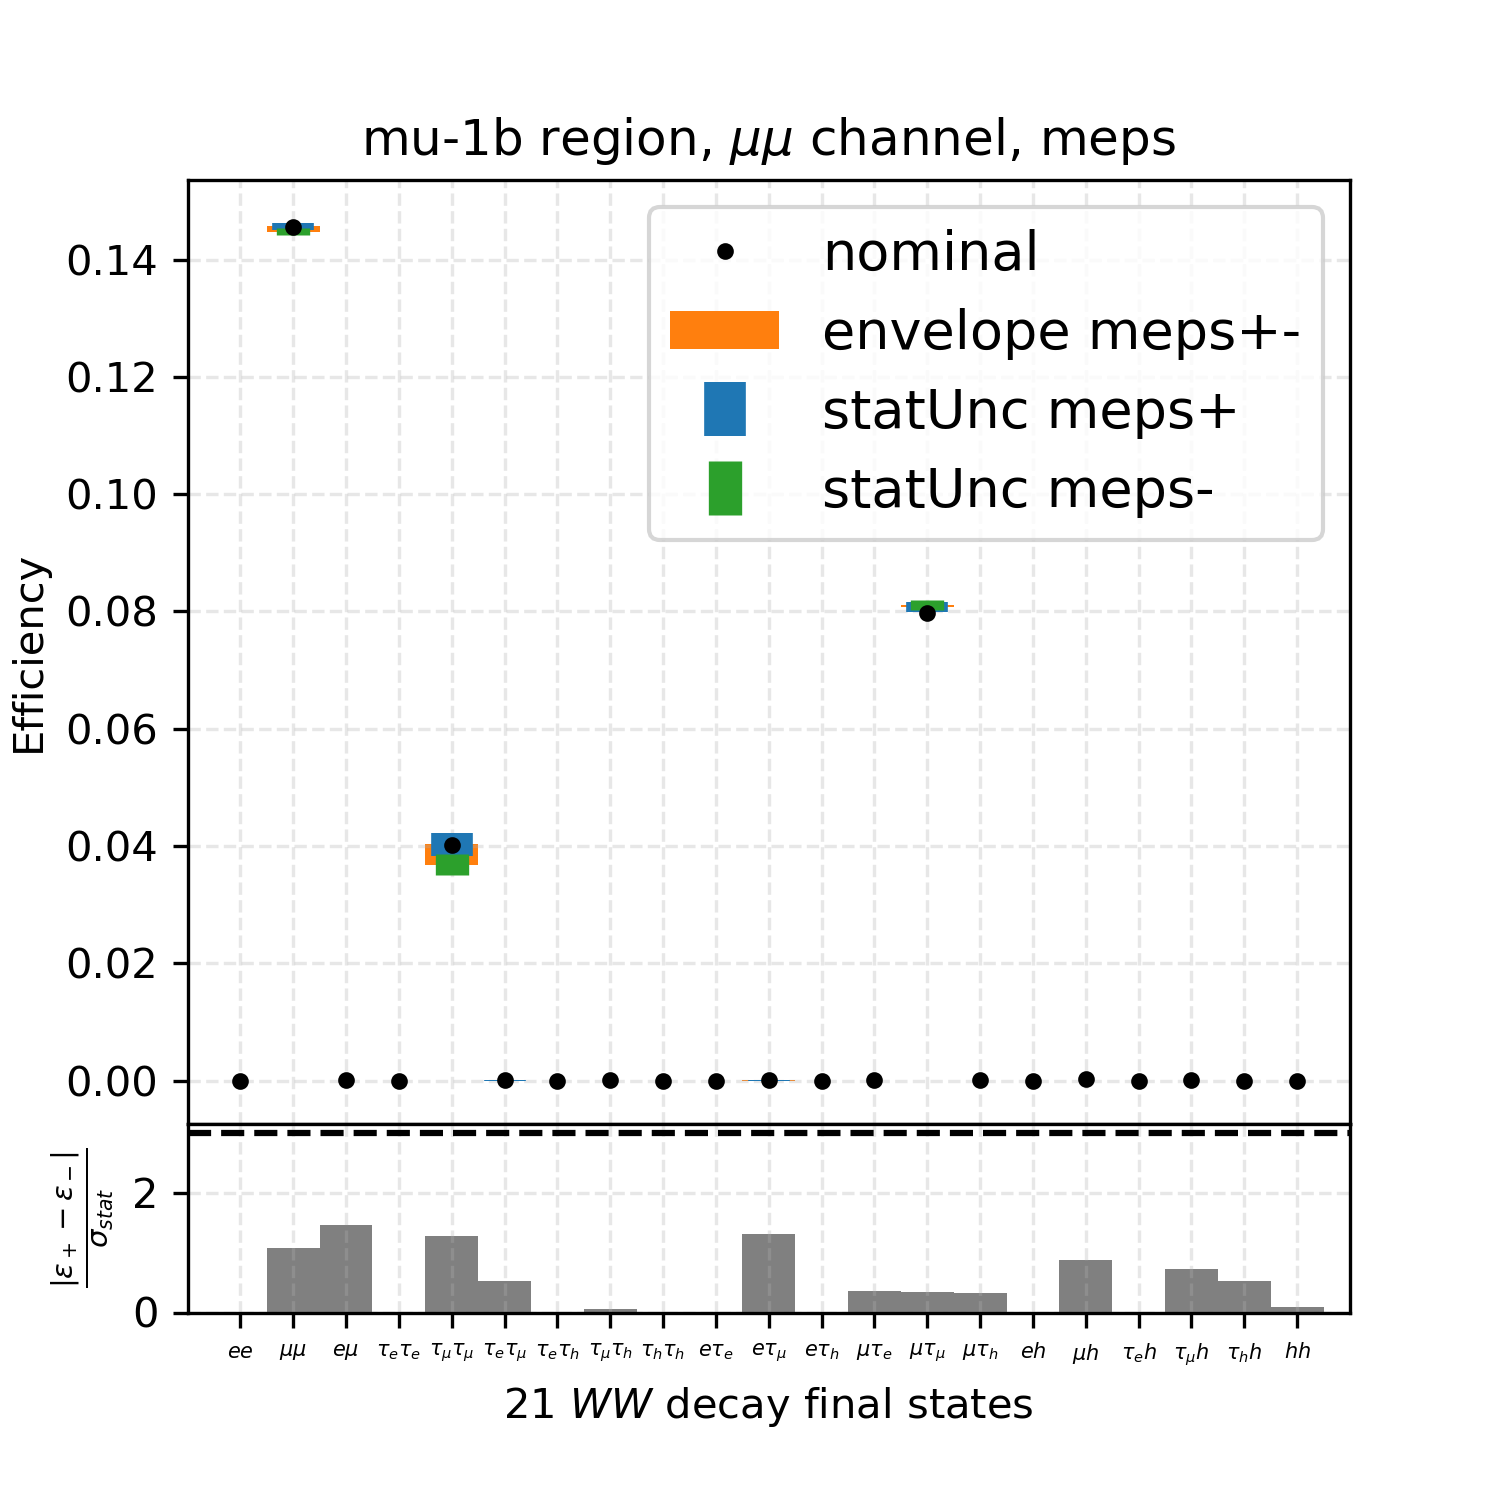
\includegraphics[width=0.24\textwidth]{chapters/Appendix/sectionTTSyst/figures/afterCorr/icata0_ch1_meps.png}
    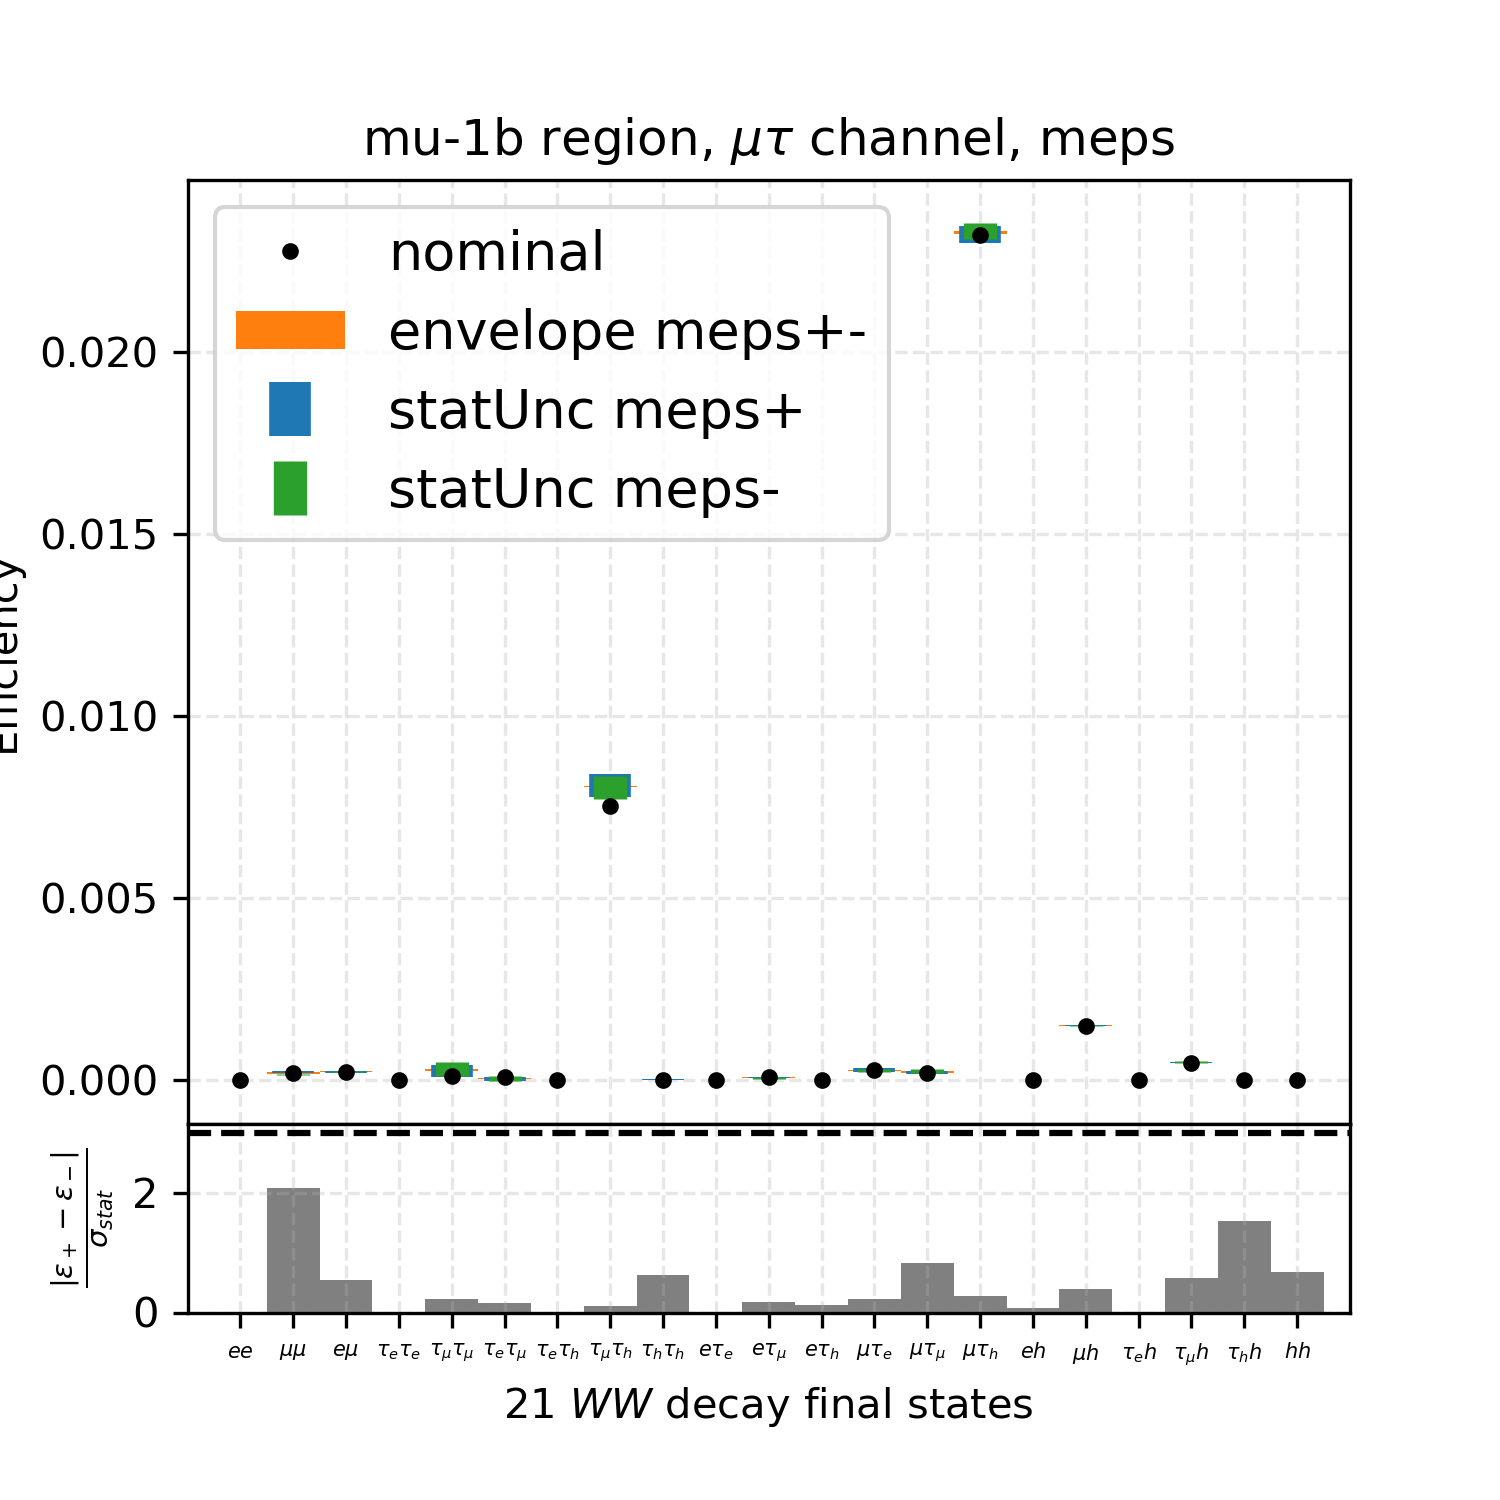
\includegraphics[width=0.24\textwidth]{chapters/Appendix/sectionTTSyst/figures/afterCorr/icata0_ch2_meps.png}
    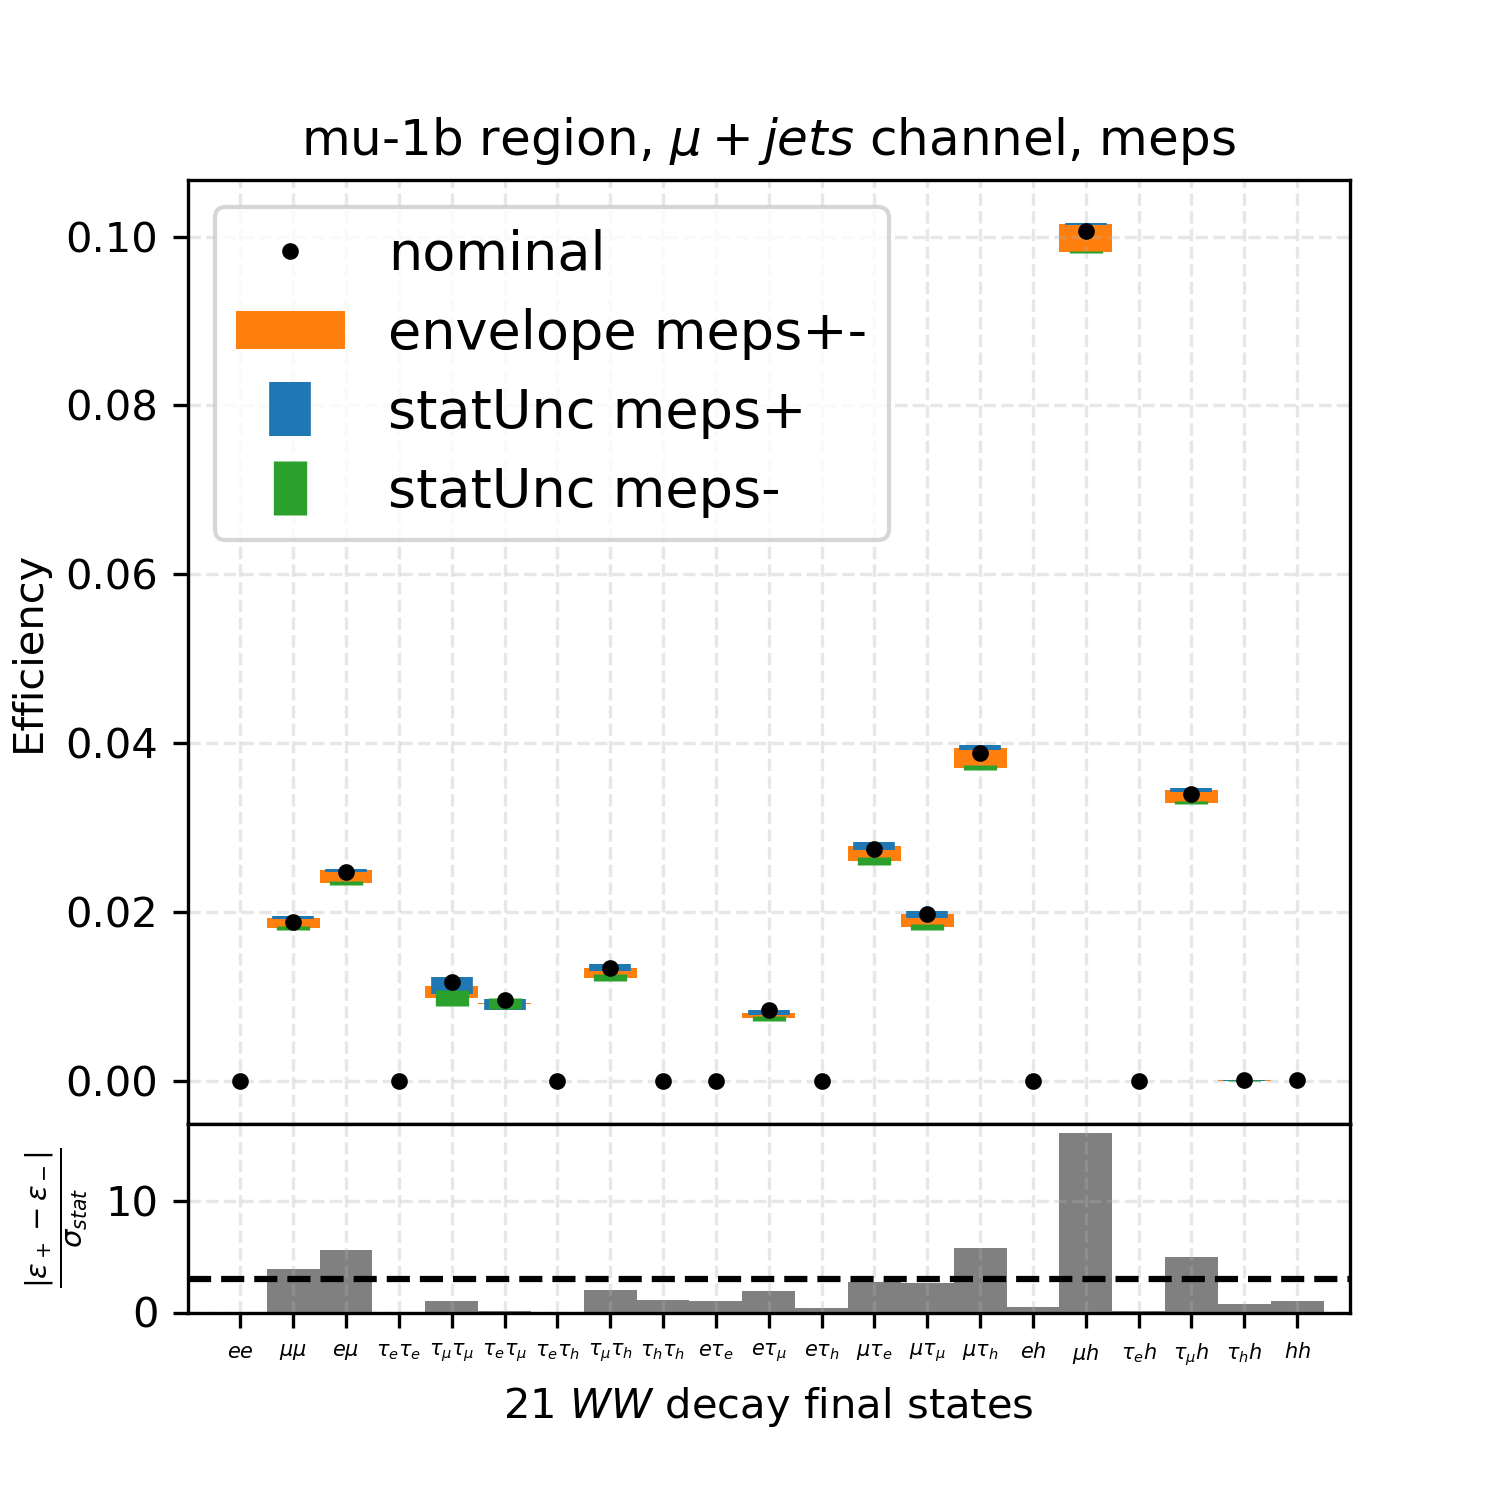
\includegraphics[width=0.24\textwidth]{chapters/Appendix/sectionTTSyst/figures/afterCorr/icata0_ch3_meps.png}

    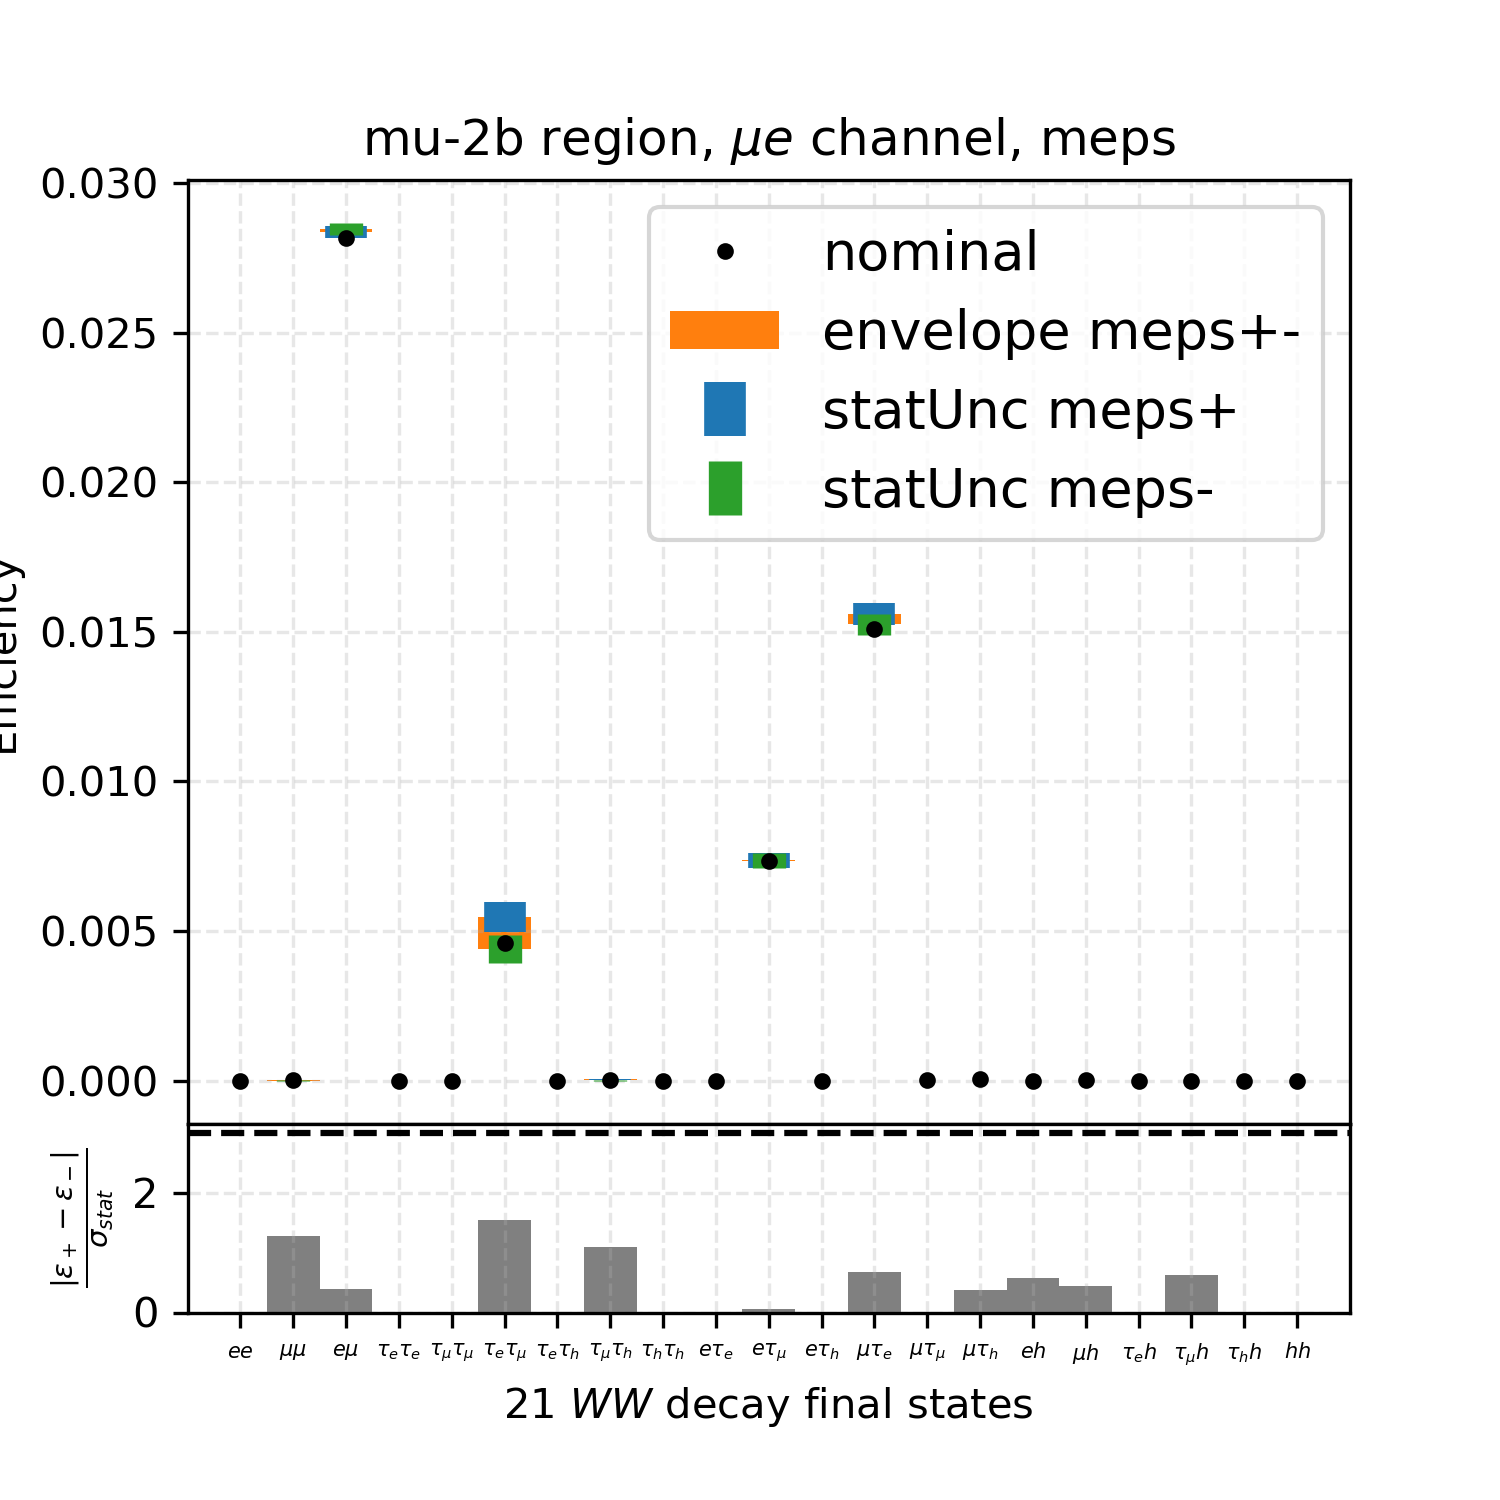
\includegraphics[width=0.24\textwidth]{chapters/Appendix/sectionTTSyst/figures/afterCorr/icata1_ch0_meps.png}
    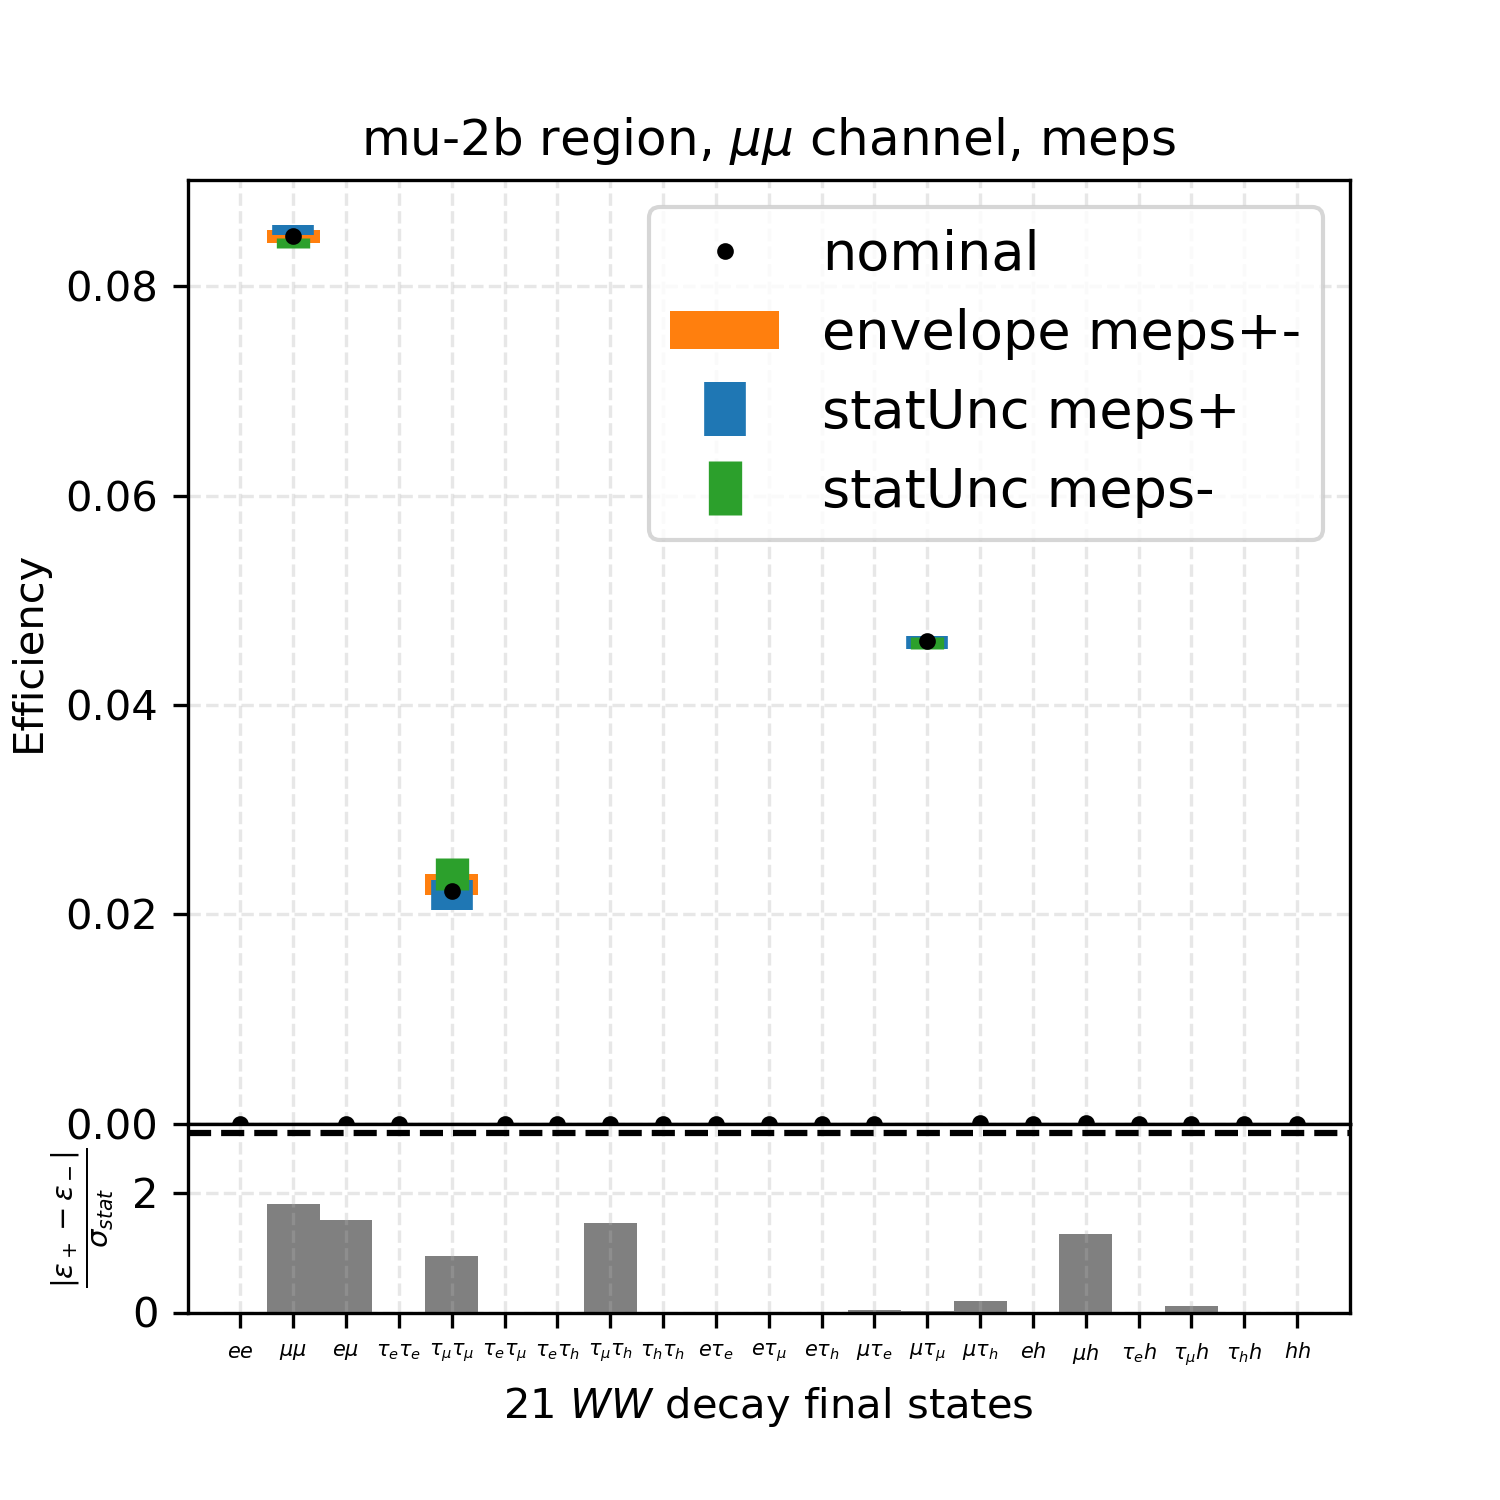
\includegraphics[width=0.24\textwidth]{chapters/Appendix/sectionTTSyst/figures/afterCorr/icata1_ch1_meps.png}
    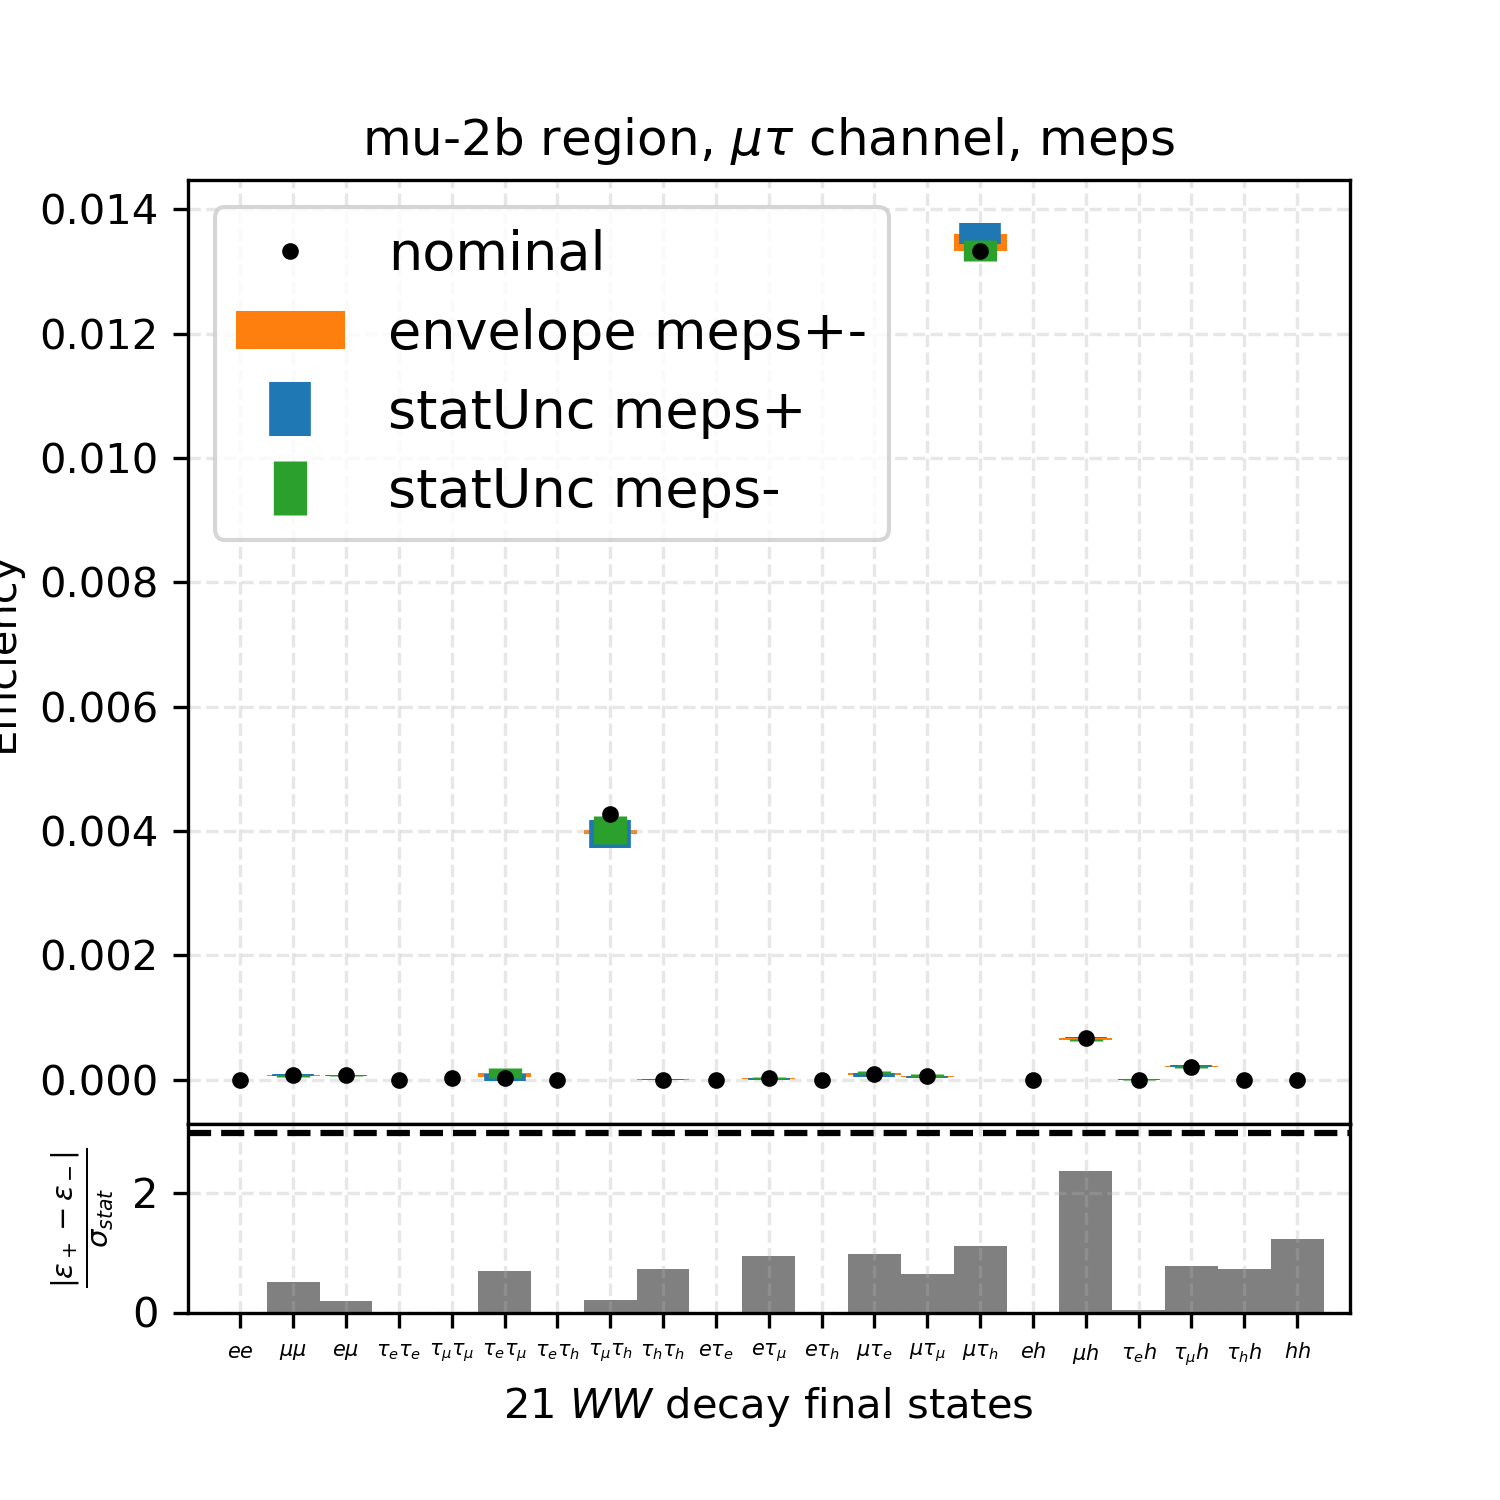
\includegraphics[width=0.24\textwidth]{chapters/Appendix/sectionTTSyst/figures/afterCorr/icata1_ch2_meps.png}
    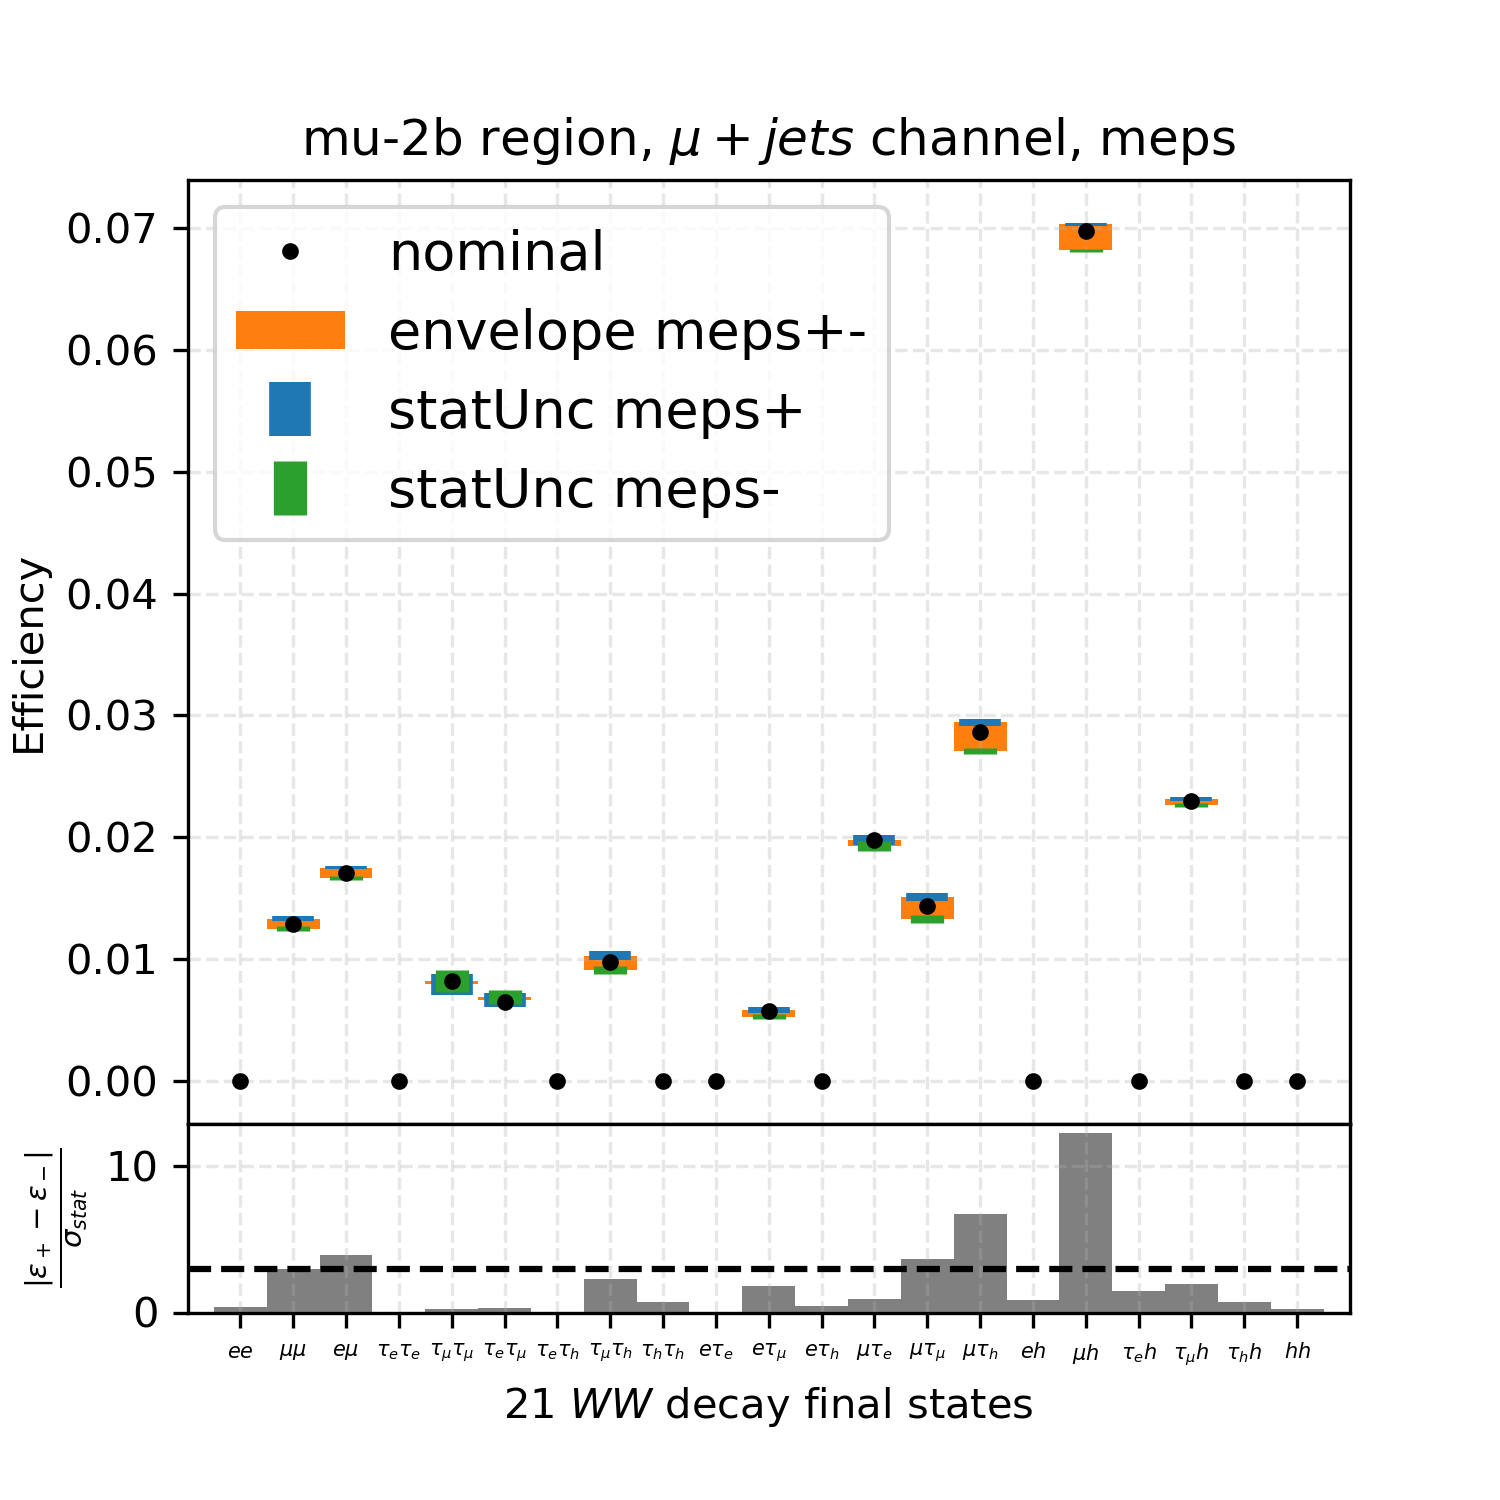
\includegraphics[width=0.24\textwidth]{chapters/Appendix/sectionTTSyst/figures/afterCorr/icata1_ch3_meps.png}
    
    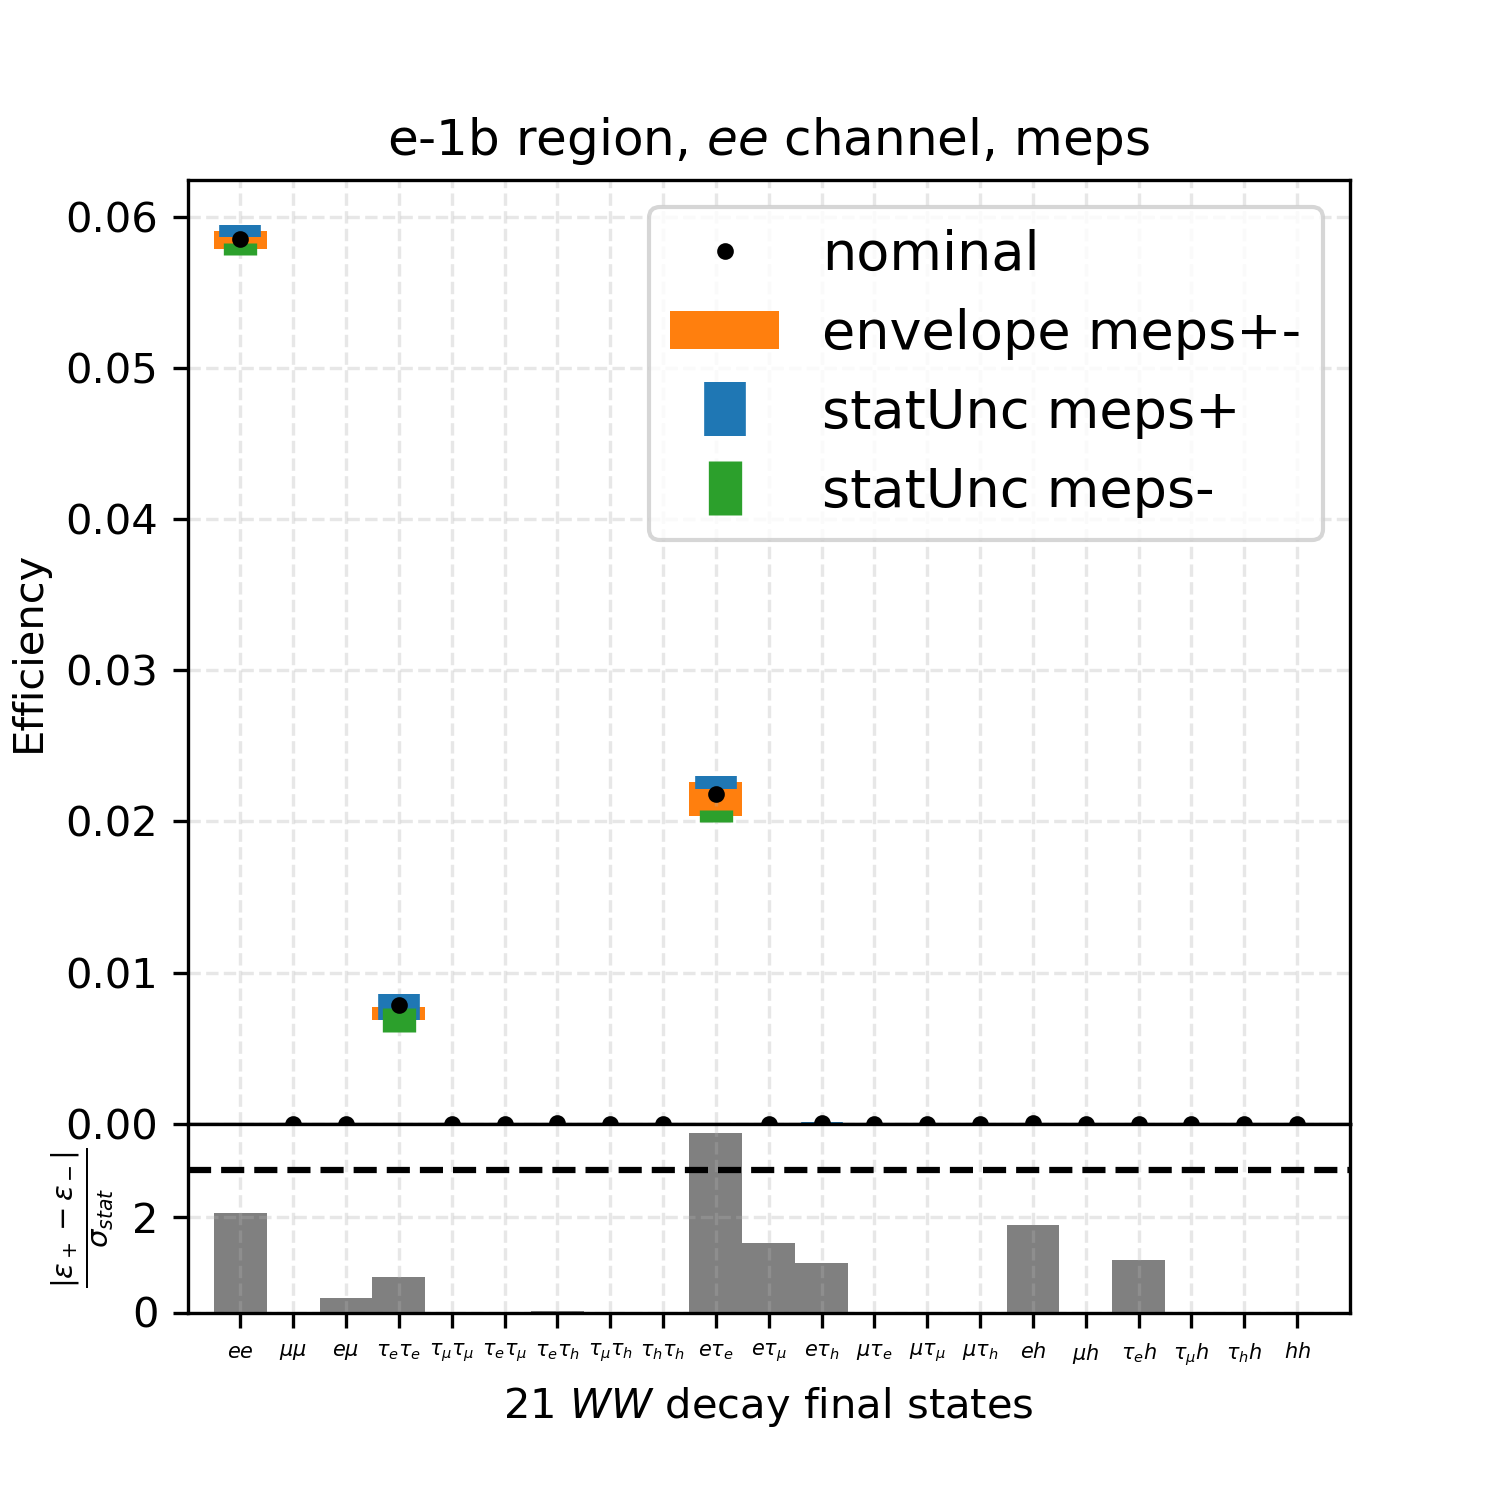
\includegraphics[width=0.24\textwidth]{chapters/Appendix/sectionTTSyst/figures/afterCorr/icata2_ch0_meps.png}
    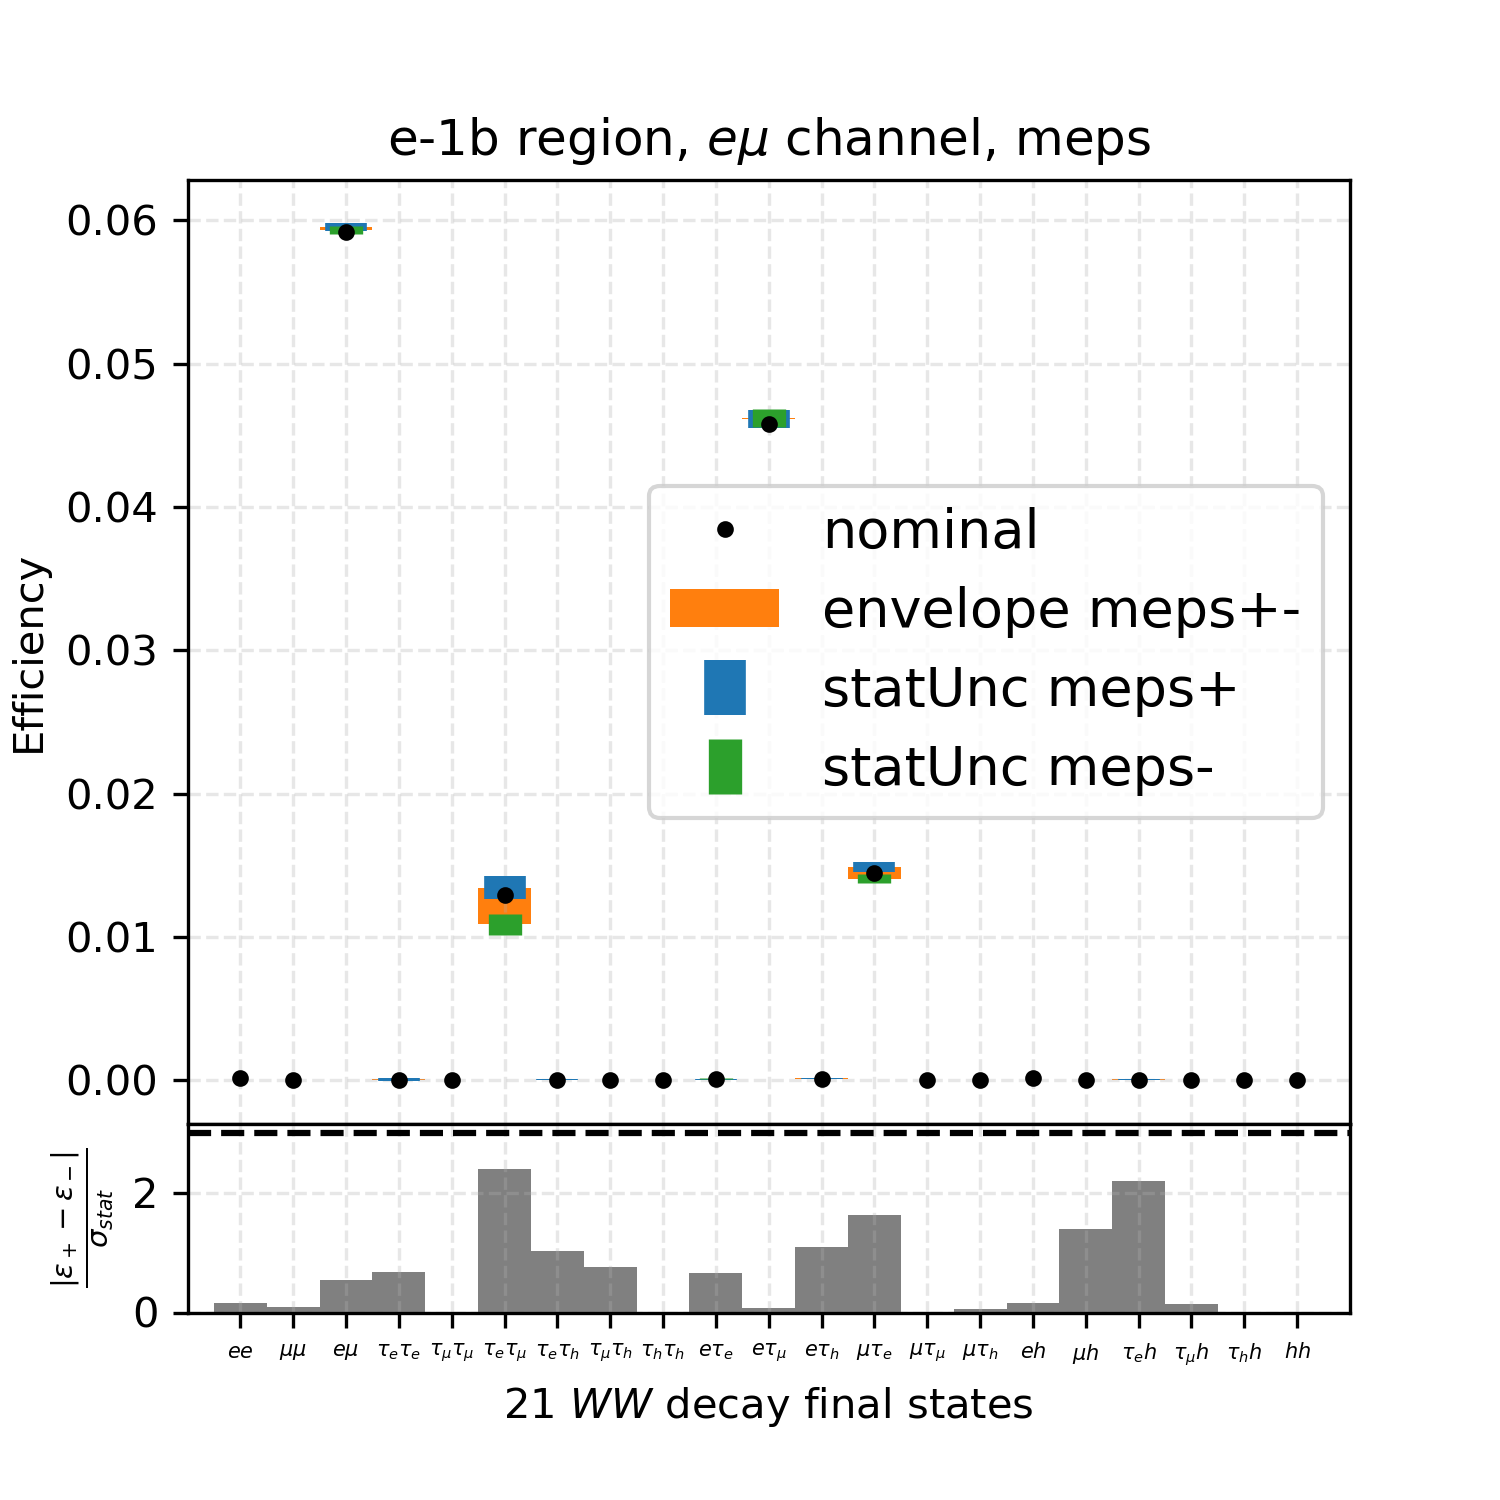
\includegraphics[width=0.24\textwidth]{chapters/Appendix/sectionTTSyst/figures/afterCorr/icata2_ch1_meps.png}
    \includegraphics[width=0.24\textwidth]{chapters/Appendix/sectionTTSyst/figures/afterCorr/icata2_ch2_meps.png}
    \includegraphics[width=0.24\textwidth]{chapters/Appendix/sectionTTSyst/figures/afterCorr/icata2_ch3_meps.png}

    \includegraphics[width=0.24\textwidth]{chapters/Appendix/sectionTTSyst/figures/afterCorr/icata3_ch0_meps.png}
    \includegraphics[width=0.24\textwidth]{chapters/Appendix/sectionTTSyst/figures/afterCorr/icata3_ch1_meps.png}
    \includegraphics[width=0.24\textwidth]{chapters/Appendix/sectionTTSyst/figures/afterCorr/icata3_ch2_meps.png}
    \includegraphics[width=0.24\textwidth]{chapters/Appendix/sectionTTSyst/figures/afterCorr/icata3_ch3_meps.png}
    
    \caption{Reweight $\tau_h$ and $j \to \tau_h$ efficiencies in the dedicated FSR, ISF, MEPS, UE ttbar samples}
    \label{fig:appendix:reweighttt:effAfterCorrFSR}
\end{figure}


\begin{figure}
    \centering
    \includegraphics[width=0.24\textwidth]{chapters/Appendix/sectionTTSyst/figures/afterCorr/icata0_ch0_ue.png}
    \includegraphics[width=0.24\textwidth]{chapters/Appendix/sectionTTSyst/figures/afterCorr/icata0_ch1_ue.png}
    \includegraphics[width=0.24\textwidth]{chapters/Appendix/sectionTTSyst/figures/afterCorr/icata0_ch2_ue.png}
    \includegraphics[width=0.24\textwidth]{chapters/Appendix/sectionTTSyst/figures/afterCorr/icata0_ch3_ue.png}

    \includegraphics[width=0.24\textwidth]{chapters/Appendix/sectionTTSyst/figures/afterCorr/icata1_ch0_ue.png}
    \includegraphics[width=0.24\textwidth]{chapters/Appendix/sectionTTSyst/figures/afterCorr/icata1_ch1_ue.png}
    \includegraphics[width=0.24\textwidth]{chapters/Appendix/sectionTTSyst/figures/afterCorr/icata1_ch2_ue.png}
    \includegraphics[width=0.24\textwidth]{chapters/Appendix/sectionTTSyst/figures/afterCorr/icata1_ch3_ue.png}
    
    \includegraphics[width=0.24\textwidth]{chapters/Appendix/sectionTTSyst/figures/afterCorr/icata2_ch0_ue.png}
    \includegraphics[width=0.24\textwidth]{chapters/Appendix/sectionTTSyst/figures/afterCorr/icata2_ch1_ue.png}
    \includegraphics[width=0.24\textwidth]{chapters/Appendix/sectionTTSyst/figures/afterCorr/icata2_ch2_ue.png}
    \includegraphics[width=0.24\textwidth]{chapters/Appendix/sectionTTSyst/figures/afterCorr/icata2_ch3_ue.png}

    \includegraphics[width=0.24\textwidth]{chapters/Appendix/sectionTTSyst/figures/afterCorr/icata3_ch0_ue.png}
    \includegraphics[width=0.24\textwidth]{chapters/Appendix/sectionTTSyst/figures/afterCorr/icata3_ch1_ue.png}
    \includegraphics[width=0.24\textwidth]{chapters/Appendix/sectionTTSyst/figures/afterCorr/icata3_ch2_ue.png}
    \includegraphics[width=0.24\textwidth]{chapters/Appendix/sectionTTSyst/figures/afterCorr/icata3_ch3_ue.png}
    
    \caption{Reweight $\tau_h$ and $j \to \tau_h$ efficiencies in the dedicated FSR, ISF, MEPS, UE ttbar samples}
    \label{fig:appendix:reweighttt:effAfterCorrFSR}
\end{figure}

